% **************************************************************************************************************
% A Classic Thesis Style
% Copyright (C) 2018 André Miede and Ivo Pletikosić
% **************************************************************************************************************
%\RequirePackage{silence} % :-\
%    \WarningFilter{scrreprt}{Usage of package `titlesec'}
%    %\WarningFilter{scrreprt}{Activating an ugly workaround}
%    \WarningFilter{titlesec}{Non standard sectioning command detected}
\documentclass[ %twoside,
                oneside,
                openright,titlepage,numbers=noenddot,%1headlines,
                headinclude,footinclude,cleardoublepage=empty,abstract=on,
                %BCOR=5mm,
                paper=a4,fontsize=11pt
                ]{scrreprt}

%********************************************************************
% Note: Make all your adjustments in here
%*******************************************************
% ****************************************************************************************************
% classicthesis-config.tex
% formerly known as loadpackages.sty, classicthesis-ldpkg.sty, and classicthesis-preamble.sty
% Use it at the beginning of your ClassicThesis.tex, or as a LaTeX Preamble
% in your ClassicThesis.{tex,lyx} with % ****************************************************************************************************
% classicthesis-config.tex
% formerly known as loadpackages.sty, classicthesis-ldpkg.sty, and classicthesis-preamble.sty
% Use it at the beginning of your ClassicThesis.tex, or as a LaTeX Preamble
% in your ClassicThesis.{tex,lyx} with % ****************************************************************************************************
% classicthesis-config.tex
% formerly known as loadpackages.sty, classicthesis-ldpkg.sty, and classicthesis-preamble.sty
% Use it at the beginning of your ClassicThesis.tex, or as a LaTeX Preamble
% in your ClassicThesis.{tex,lyx} with \input{classicthesis-config}
% ****************************************************************************************************
% If you like the classicthesis, then I would appreciate a postcard.
% My address can be found in the file ClassicThesis.pdf. A collection
% of the postcards I received so far is available online at
% http://postcards.miede.de
% ****************************************************************************************************


% ****************************************************************************************************
% 0. Set the encoding of your files. UTF-8 is the only sensible encoding nowadays. If you can't read
% äöüßáéçèê∂åëæƒÏ€ then change the encoding setting in your editor, not the line below. If your editor
% does not support utf8 use another editor!
% ****************************************************************************************************
\PassOptionsToPackage{utf8}{inputenc}
  \usepackage{inputenc}

\PassOptionsToPackage{T1}{fontenc} % T2A for cyrillics
  \usepackage{fontenc}


% ****************************************************************************************************
% 1. Configure classicthesis for your needs here, e.g., remove "drafting" below
% in order to deactivate the time-stamp on the pages
% (see ClassicThesis.pdf for more information):
% ****************************************************************************************************
\PassOptionsToPackage{
  drafting=true,    % print version information on the bottom of the pages
  tocaligned=false, % the left column of the toc will be aligned (no indentation)
  dottedtoc=false,  % page numbers in ToC flushed right
  eulerchapternumbers=true, % use AMS Euler for chapter font (otherwise Palatino)
  linedheaders=false,       % chaper headers will have line above and beneath
  floatperchapter=true,     % numbering per chapter for all floats (i.e., Figure 1.1)
  eulermath=false,  % use awesome Euler fonts for mathematical formulae (only with pdfLaTeX)
  beramono=true,    % toggle a nice monospaced font (w/ bold)
  palatino=true,    % deactivate standard font for loading another one, see the last section at the end of this file for suggestions
  style=classicthesis % classicthesis, arsclassica
}{classicthesis}


% ****************************************************************************************************
% 2. Personal data and user ad-hoc commands (insert your own data here)
% ****************************************************************************************************
\newcommand{\myTitle}{Zur Theorie der ordinären Entitäten des Brentanoraumes\xspace}
% \newcommand{\mySubtitle}{Ein topologischer Interpretationsansatz\xspace}
\newcommand{\mySubtitle}{Ein repräsentantenbasierter Interpretationsansatz\xspace}
\newcommand{\myDegree}{Bachelor of science\xspace}
\newcommand{\myName}{Bärbel Hanle\xspace}
\newcommand{\mybirthday}{06.02.1982}
\newcommand{\mybirthtown}{Stuttgart}
\newcommand{\mybirthcountry}{Deutschland}
\newcommand{\myProf}{Dr. Frank Loebe\xspace}
\newcommand{\myOtherProf}{Dr. habil. Ringo Baumann\xspace}
\newcommand{\mySupervisor}{\xspace}
\newcommand{\myFaculty}{Institut für Mathematik und Informatik\xspace}
\newcommand{\myDepartment}{\xspace}
\newcommand{\myUni}{Universität Leipzig\xspace}
\newcommand{\myLocation}{Leipzig\xspace}
\newcommand{\myTime}{10.05.2022\xspace} 
\newcommand{\myVersion}{\classicthesis}

% ********************************************************************
% Setup, finetuning, and useful commands
% ********************************************************************
\providecommand{\mLyX}{L\kern-.1667em\lower.25em\hbox{Y}\kelastrn-.125emX\@}
\newcommand{\ie}{i.\,e.}
\newcommand{\Ie}{I.\,e.}
\newcommand{\eg}{e.\,g.}
\newcommand{\Eg}{E.\,g.}
% ****************************************************************************************************


% ****************************************************************************************************
% 3. Loading some handy packages
% ****************************************************************************************************
% ********************************************************************
% Packages with options that might require adjustments
% ********************************************************************
\PassOptionsToPackage{american,ngerman}{babel} % change this to your language(s), main language last
% Spanish languages need extra options in order to work with this template
%\PassOptionsToPackage{spanish,es-lcroman}{babel}
    \usepackage{babel}

\usepackage{csquotes}
\PassOptionsToPackage{%
  %backend=biber,bibencoding=utf8, %instead of bibtex
  backend=bibtex8,bibencoding=ascii,%
  language=auto,%
  style=authoryear,dashed=false%
  %style=authoryear-comp, % Author 1999, 2010
  %bibstyle=authoryear,dashed=false, % dashed: substitute rep. author with ---
  sorting=nyt, % name, year, title
  maxbibnames=10, % default: 3, et al.
  %backref=true,%
  natbib=true % natbib compatibility mode (\citep and \citet still work)
}{biblatex}
    \usepackage{biblatex}

\PassOptionsToPackage{fleqn}{amsmath}       % math environments and more by the AMS
  \usepackage{amsmath}

% ********************************************************************
% General useful packages
% ********************************************************************
\usepackage{graphicx} %
\usepackage{scrhack} % fix warnings when using KOMA with listings package
\usepackage{xspace} % to get the spacing after macros right

%\usepackage{textcase}
\PassOptionsToPackage{printonlyused,smaller}{acronym}
  \usepackage{acronym} % nice macros for handling all acronyms in the thesis
  %\renewcommand{\bflabel}[1]{{#1}\hfill} % fix the list of acronyms --> no longer working
  %\renewcommand*{\acsfont}[1]{\textsc{#1}}
  %\renewcommand*{\aclabelfont}[1]{\acsfont{#1}}
  %\def\bflabel#1{{#1\hfill}}
  \def\bflabel#1{{\acsfont{#1}\hfill}}
  \def\aclabelfont#1{\acsfont{#1}}
  
  %\renewcommand{\acsfont}[1]{{\scshape \MakeTextLowercase{#1}}}
  
\PassOptionsToPackage{activate={true,nocompatibility},final,tracking=true,kerning=true,spacing=true,factor=1100,stretch=10,shrink=10,final}{microtype}%final-even in draft mode
\usepackage[]{microtype}
% ****************************************************************************************************
%\usepackage{pgfplots} % External TikZ/PGF support (thanks to Andreas Nautsch)
%\usetikzlibrary{external}
%\tikzexternalize[mode=list and make, prefix=ext-tikz/]
% ****************************************************************************************************

% ****************************************************************************************************
% 4. Setup floats: tables, (sub)figures, and captions
% ****************************************************************************************************
\usepackage{tabularx} % better tables
  \setlength{\extrarowheight}{3pt} % increase table row height
\newcommand{\tableheadline}[1]{\multicolumn{1}{l}{\spacedlowsmallcaps{#1}}}
\newcommand{\myfloatalign}{\centering} % to be used with each float for alignment
\usepackage{subfig}
% ****************************************************************************************************


% ****************************************************************************************************
% 5. Setup code listings
% ****************************************************************************************************
\usepackage{listings}
%\lstset{emph={trueIndex,root},emphstyle=\color{BlueViolet}}%\underbar} % for special keywords
\lstset{language=[LaTeX]Tex,%C++,
  morekeywords={PassOptionsToPackage,selectlanguage},
  keywordstyle=\color{RoyalBlue},%\bfseries,
  basicstyle=\small\ttfamily,
  %identifierstyle=\color{NavyBlue},
  commentstyle=\color{Green}\ttfamily,
  stringstyle=\rmfamily,
  numbers=none,%left,%
  numberstyle=\scriptsize,%\tiny
  stepnumber=5,
  numbersep=8pt,
  showstringspaces=false,
  breaklines=true,
  %frameround=ftff,
  %frame=single,
  belowcaptionskip=.75\baselineskip
  %frame=L
}
% ****************************************************************************************************




% ****************************************************************************************************
% 6. Last calls before the bar closes
% ****************************************************************************************************
% ********************************************************************
% Her Majesty herself
% ********************************************************************
\usepackage[dottedtoc]{classicthesis}


% ********************************************************************
% Fine-tune hyperreferences (hyperref should be called last)
% ********************************************************************
\hypersetup{%
  %draft, % hyperref's draft mode, for printing see below
  colorlinks=true, linktocpage=true, pdfstartpage=3, pdfstartview=FitV,%
  % uncomment the following line if you want to have black links (e.g., for printing)
  %colorlinks=false, linktocpage=false, pdfstartpage=3, pdfstartview=FitV, pdfborder={0 0 0},%
  breaklinks=true, pageanchor=true,%
  pdfpagemode=UseNone, %
  % pdfpagemode=UseOutlines,%
  plainpages=false, bookmarksnumbered, bookmarksopen=true, bookmarksopenlevel=1,%
  hypertexnames=true, pdfhighlight=/O,%nesting=true,%frenchlinks,%
  urlcolor=CTurl, linkcolor=CTlink, citecolor=CTcitation, %pagecolor=RoyalBlue,%
  %urlcolor=Black, linkcolor=Black, citecolor=Black, %pagecolor=Black,%
  pdftitle={\myTitle},%
  pdfauthor={\textcopyright\ \myName, \myUni, \myFaculty},%
  pdfsubject={},%
  pdfkeywords={},%
  pdfcreator={pdfLaTeX},%
  pdfproducer={LaTeX with hyperref and classicthesis}%
}

%**************************************************************************
% Eigene Pakete
%**************************************************************************
\usepackage{amssymb} % für \varnothing
\usepackage{stmaryrd} % Widerspruchsblitz
\usepackage{amsthm} % Für Theoremumgebungen
  \usepackage{zref-perpage} % FL: zref-perpage is there for 
    % fixing a MikTeX problem with zref, which is loaded by mdframed;
	  % cf. https://github.com/ho-tex/zref/issues/14
\usepackage[framemethod=tikz]{mdframed} % Rand für Theoreme
\usepackage{multirow}
\usepackage{makecell} % Zeilenumburuch innerhalb einer Zelle
\usepackage{longtable} % Tabelle über mehrere Seiten´
\usepackage{subcaption}
% \usepackage[labelformat=parens,labelsep=quad,skip=3pt]{caption}
%\usepackage{graphicx}

%\usepackage{textcase}



% ********************************************************************
% Setup autoreferences (hyperref and babel)
% ********************************************************************
% There are some issues regarding autorefnames
% http://www.tex.ac.uk/cgi-bin/texfaq2html?label=latexwords
% you have to redefine the macros for the
% language you use, e.g., american, ngerman
% (as chosen when loading babel/AtBeginDocument)
% ********************************************************************
\makeatletter
\@ifpackageloaded{babel}%
  {%
    \addto\extrasamerican{%
		  \renewcommand*{\figurename}{Fig.}%
      \renewcommand*{\figureautorefname}{Figure}%
      \renewcommand*{\tableautorefname}{Table}%
      \renewcommand*{\partautorefname}{Part}%
      \renewcommand*{\chapterautorefname}{Chapter}%
      \renewcommand*{\sectionautorefname}{Section}%
      \renewcommand*{\subsectionautorefname}{Section}%
      \renewcommand*{\subsubsectionautorefname}{Section}%
    }%
    \addto\extrasngerman{%
		  \renewcommand*{\figurename}{Abb.}%
      \renewcommand*{\paragraphautorefname}{Absatz}%
      \renewcommand*{\subparagraphautorefname}{Unterabsatz}%
      \renewcommand*{\footnoteautorefname}{Fu\"snote}%
      \renewcommand*{\FancyVerbLineautorefname}{Zeile}%
      \renewcommand*{\theoremautorefname}{Theorem}%
      \renewcommand*{\appendixautorefname}{Anhang}%
      \renewcommand*{\equationautorefname}{Gleichung}%
      \renewcommand*{\itemautorefname}{Punkt}%
    }%
      % Fix to getting autorefs for subfigures right (thanks to Belinda Vogt for changing the definition)
      \providecommand{\subfigureautorefname}{\figureautorefname}%
    }{\relax}
\makeatother


% ********************************************************************
% Development Stuff
% ********************************************************************
\listfiles
%\PassOptionsToPackage{l2tabu,orthodox,abort}{nag}
%  \usepackage{nag}
%\PassOptionsToPackage{warning, all}{onlyamsmath}
%  \usepackage{onlyamsmath}


% ****************************************************************************************************
% 7. Further adjustments (experimental)
% ****************************************************************************************************
% ********************************************************************
% Changing the text area
% ********************************************************************
%\areaset[current]{312pt}{761pt} % 686 (factor 2.2) + 33 head + 42 head \the\footskip
%\setlength{\marginparwidth}{7em}%
%\setlength{\marginparsep}{2em}%

% ********************************************************************
% Using different fonts
% ********************************************************************
%\usepackage[oldstylenums]{kpfonts} % oldstyle notextcomp
% \usepackage[osf]{libertine}
%\usepackage[light,condensed,math]{iwona}
%\renewcommand{\sfdefault}{iwona}
%\usepackage{lmodern} % <-- no osf support :-(
%\usepackage{cfr-lm} %
%\usepackage[urw-garamond]{mathdesign} <-- no osf support :-(
%\usepackage[default,osfigures]{opensans} % scale=0.95
%\usepackage[sfdefault]{FiraSans}
% \usepackage[opticals,mathlf]{MinionPro} % onlytext
% ********************************************************************
%\usepackage[largesc,osf]{newpxtext}
%\linespread{1.05} % a bit more for Palatino
% Used to fix these:
% https://bitbucket.org/amiede/classicthesis/issues/139/italics-in-pallatino-capitals-chapter
% https://bitbucket.org/amiede/classicthesis/issues/45/problema-testatine-su-classicthesis-style
% ********************************************************************
% ****************************************************************************************************

% ****** Custom
%\usepackage[disable]{todonotes}
\usepackage{todonotes}
\usepackage{cleveref}

%***************************************************************************
% Umgebungen
%***************************************************************************
\theoremstyle{definition}

\newtheorem{dfn}{Def}[section]
\newtheorem{nota}[dfn]{Notation}
\newtheorem{konv}[dfn]{Konvention}

\newtheorem{satz}[dfn]{Satz}
\newtheorem{kor}[dfn]{Kor}
\newtheorem{hyp}[dfn]{Hyp}

\newtheorem{bsp}[dfn]{Bsp}
\newtheorem{gegenbsp}[dfn]{Gegenbeispiel}
\newtheorem{bem}[dfn]{Bem}
\newtheorem*{erin}{Erinnerung}
\newtheorem*{bew}{Bew}
\newtheorem*{bewidee}{Beweisidee}

\mdfdefinestyle{grey}{
    skipabove=5pt,
    skipbelow=5pt,
    innerbottommargin=12pt,
    %innerleftmargin=20pt
    innerrightmargin=20pt
    leftmargin=5pt,
    rightmargin=5pt,
    %linewidth=0.2pt,
    roundcorner=2pt,
    backgroundcolor=black!5,
    hidealllines=true,
    needspace=60pt,
		aftersingleframe={\noindent},
}

\mdfdefinestyle{white}{
    skipabove=5pt,
    skipbelow=5pt,
    innerbottommargin=12pt,
    %innerleftmargin=20pt
    innerrightmargin=20pt
    leftmargin=5pt,
    rightmargin=5pt,
    %linewidth=0.2pt,
    roundcorner=2pt,
    %backgroundcolor=black!5,
    %hidealllines=true
}

\mdfdefinestyle{beweis}{
    skipabove=0pt,
    skipbelow=5pt,
    innerbottommargin=12pt,
    %innerleftmargin=20pt
    innerrightmargin=20pt
    leftmargin=5pt,
    rightmargin=5pt,
    %linewidth=0.2pt,
    roundcorner=2pt,
    %backgroundcolor=black!5,
    %hidealllines=true
    linecolor=black!10
%     rightline=false
%     bottomline=false
%     topline=false
}

\surroundwithmdframed[style=grey]{dfn}
\surroundwithmdframed[style=grey]{nota}
\surroundwithmdframed[style=grey]{konv}
\surroundwithmdframed[style=grey]{satz}
\surroundwithmdframed[style=grey]{kor}
\surroundwithmdframed[style=grey]{hyp}
\surroundwithmdframed[style=white]{bsp}
\surroundwithmdframed[style=white]{gegenbsp}
\surroundwithmdframed[style=white]{bem}
\surroundwithmdframed[style=white]{erin}
\surroundwithmdframed[style=beweis]{bew}
\surroundwithmdframed[style=beweis]{bewidee}




\DeclareRobustCommand{\BSO}{\mathcal{BS^O}}

%--------------------------------------------

\newcommand{\thmemph}{\textbf}
\newcommand{\textemph}{\spacedlowsmallcaps}
%\renewcommand{\marginpar}[2][]{} % marginpars verstecken



%*****************************************************************************
% BS-Kommandos
%********************************************************************************
% 
% %%%%%%%%%%%%%%%%%%%%%%%%%%%%%%%%%%%%%%%%%%%%%%%%%%%%%%%%
% % OPTION uniformSymbols STARTS
% %%%%%%%%%%%%%%%%%%%%%%%%%%%%%%%%%%%%%%%%%%%%%%%%%%%%%%%%%%
% \DeclareOption{uniformSymbols}{%
% %
% \newcommand{\GSymbolFont}[1]{#1}
% %
% } %OPTION uniformSymbols ENDS HERE
% %%%%%%%%%%%%%%%%%%%%%%%%%%%%%%%%%%%%%%%%%%%%%%%%%%%
% %%%%%%%%%%%%%%%%%%%%%%%%%%%%%%%%%%%%%%%%%%%%%%%%%%% 
% 
% %%%%%%%%%%%%%%%%%%%%%%%%%%%%%%%%%%%%%%%%%%%%%%%%%%%%%%%%
% % OPTION mboxSymbols STARTS
% %%%%%%%%%%%%%%%%%%%%%%%%%%%%%%%%%%%%%%%%%%%%%%%%%%%%%%%%%%
% \DeclareOption{mboxSymbols}{%
% %
% \renewcommand{\GSymbolFont}[1]{\mbox{#1}}
% %
% } %OPTION mboxSymbols ENDS HERE
% %%%%%%%%%%%%%%%%%%%%%%%%%%%%%%%%%%%%%%%%%%%%%%%%%%%
% %%%%%%%%%%%%%%%%%%%%%%%%%%%%%%%%%%%%%%%%%%%%%%%%%%% 
% 
% %%%%%%%%%%%%%%%%%%%%%%%%%%%%%%%%%%%%%%%%%%%%%%%%%%%%%%%%
% % OPTION mboxSymbols STARTS
% %%%%%%%%%%%%%%%%%%%%%%%%%%%%%%%%%%%%%%%%%%%%%%%%%%%%%%%%%%
% \DeclareOption{italicSymbols}{%
% %
% \renewcommand{\GSymbolFont}[1]{\ensuremath{\mathit{#1}}}
% %
% } %OPTION mboxSymbols ENDS HERE
% %%%%%%%%%%%%%%%%%%%%%%%%%%%%%%%%%%%%%%%%%%%%%%%%%%%
% %%%%%%%%%%%%%%%%%%%%%%%%%%%%%%%%%%%%%%%%%%%%%%%%%%% 
% 
% % Execution of options
% \ExecuteOptions{manAxiomStyle,uniformSymbols}

\newcommand{\GSymbolFont}[1]{\ensuremath{\mathit{#1}}}
\newcommand{\AuxD}{D\hspace*{-0.25ex}}


\newcommand{\GC}{\ensuremath{\GSymbolFont{C}}}
\newcommand{\GCrossdDBn}{\ensuremath{\GSymbolFont{Cross\Gd DB_{n}}}}
\newcommand{\GCrossoneDBn}{\ensuremath{\GSymbolFont{Cross1DB_{n}}}}
\newcommand{\GCrosstwoDBn}{\ensuremath{\GSymbolFont{Cross2DB_{n}}}}
\newcommand{\GCrosszeroDBn}{\ensuremath{\GSymbolFont{Cross0DB_{n}}}}
\newcommand{\Gc}{\ensuremath{\GSymbolFont{c}}}
\newcommand{\Gcrossonedbn}{\ensuremath{\GSymbolFont{cross1db_{n}}}}
\newcommand{\Gcrosstwodbn}{\ensuremath{\GSymbolFont{cross2db_{n}}}}
%\newcommand{\Gcrosszerodb}{\ensuremath{\GSymbolFont{cross0db}}}
\newcommand{\Gcrosszerodbn}{\ensuremath{\GSymbolFont{cross0db_{n}}}}

\newcommand{\Gd}{\boldsymbol{\mathsf{d}}}
\newcommand{\Gone}{\boldsymbol{\mathsf{1}}}
\newcommand{\Gtwo}{\boldsymbol{\mathsf{2}}}
\newcommand{\Gthree}{\boldsymbol{\mathsf{3}}}
\newcommand{\GdD}{\ensuremath{\GSymbolFont{\Gd D}}}
\newcommand{\GdDB}{\ensuremath{\GSymbolFont{\Gd\AuxD B}}}
\newcommand{\GdDC}{\ensuremath{\GSymbolFont{\Gd\AuxD C}}}
\newcommand{\GdDE}{\ensuremath{\GSymbolFont{\Gd\AuxD E}}}
\newcommand{\Gddb}{\ensuremath{\GSymbolFont{\Gd db}}}
\newcommand{\Gddhypp}{\ensuremath{\GSymbolFont{\Gd dhypp}}}
\newcommand{\Gdmdhypp}{\ensuremath{\GSymbolFont{\Gdm dhypp}}}
\newcommand{\Gdircomp}{\ensuremath{\GSymbolFont{dircomp}}}
\newcommand{\Gddircomp}{\ensuremath{\GSymbolFont{\Gd dircomp}}}
\newcommand{\dircomp}{\ensuremath{\GSymbolFont{\Gdp dircomp}}}
\newcommand{\Gdp}{\boldsymbol{\mathsf{(d+1)}}}
\newcommand{\Gdm}{\boldsymbol{\mathsf{(d-1)}}}

\newcommand{\GExOrd}{\ensuremath{\GSymbolFont{ExOrd}}}
\newcommand{\Gequ}{\ensuremath{\GSymbolFont{equ}}}
\newcommand{\Geqdim}{\ensuremath{\GSymbolFont{eqdim}}}
\newcommand{\Gexc}{\ensuremath{\GSymbolFont{exc}}}

\newcommand{\GGrSB}{\ensuremath{\GSymbolFont{Gr\hspace*{-0.25ex}SB}}}
\newcommand{\Ggrsb}{\ensuremath{\GSymbolFont{gr\hspace*{-0.25ex}sb}}}

\newcommand{\Ghypp}{\ensuremath{\GSymbolFont{hypp}}}

\newcommand{\GiCCDd}{\ensuremath{\GSymbolFont{i}_{\Gd}\GSymbolFont{CC}}}
\newcommand{\GiCCDone}{\ensuremath{\GSymbolFont{i}_{1}\GSymbolFont{CC}}}
\newcommand{\GiCCDtwo}{\ensuremath{\GSymbolFont{i}_{2}\GSymbolFont{CC}}}
\newcommand{\GiCCDzero}{\ensuremath{\GSymbolFont{i}_{0}\GSymbolFont{CC}}}
\newcommand{\Ginpart}{\ensuremath{\GSymbolFont{inpart}}}
\newcommand{\Gintersect}{\ensuremath{\GSymbolFont{intsect}}}
\newcommand{\Gintersectn}{\ensuremath{\GSymbolFont{intsect_{n}}}}

\newcommand{\GLDE}{\ensuremath{\GSymbolFont{LDE}}}

\newcommand{\Gcont}{\ensuremath{\GSymbolFont{cont}}}
\newcommand{\Gstrictsb}{\ensuremath{\GSymbolFont{strictsb}}}
\newcommand{\Gweaksb}{\ensuremath{\GSymbolFont{weaksb}}}

%\newcommand{\GkCCDd}{\ensuremath{\GSymbolFont{k}_{\Gd}\GSymbolFont{CC}}}
%\newcommand{\GkCCDone}{\ensuremath{\GSymbolFont{k}_{1}\GSymbolFont{CC}}}
%\newcommand{\GkCCDtwo}{\ensuremath{\GSymbolFont{k}_{2}\GSymbolFont{CC}}}
\newcommand{\GkCCDzero}{\ensuremath{\GSymbolFont{k}_{0}\GSymbolFont{CC}}}

%\newcommand{\GlCCDd}{\ensuremath{\GSymbolFont{l}_{\Gd}\GSymbolFont{CC}}}
\newcommand{\GlCCDone}{\ensuremath{\GSymbolFont{l}_{1}\GSymbolFont{CC}}}
%\newcommand{\GlCCDtwo}{\ensuremath{\GSymbolFont{l}_{2}\GSymbolFont{CC}}}
%\newcommand{\GlCCDzero}{\ensuremath{\GSymbolFont{l}_{0}\GSymbolFont{CC}}}

\newcommand{\GnCCDd}{\ensuremath{\GSymbolFont{n}_{\Gd}\GSymbolFont{CC}}}
\newcommand{\GnCCDone}{\ensuremath{\GSymbolFont{n}_{1}\GSymbolFont{CC}}}
\newcommand{\GnCCDtwo}{\ensuremath{\GSymbolFont{n}_{2}\GSymbolFont{CC}}}
\newcommand{\GnCCDzero}{\ensuremath{\GSymbolFont{n}_{0}\GSymbolFont{CC}}}
%\newcommand{\GnminusiCCDd}{\ensuremath{\GSymbolFont{(n-i)}_{\Gd}\GSymbolFont{CC}}}
\newcommand{\GnminusiCCDone}{\ensuremath{\GSymbolFont{(n-i)}_{1}\GSymbolFont{CC}}}
%\newcommand{\GnminusiCCDtwo}{\ensuremath{\GSymbolFont{(n-i)}_{2}\GSymbolFont{CC}}}
\newcommand{\GnminusiCCDzero}{\ensuremath{\GSymbolFont{(n-i)}_{0}\GSymbolFont{CC}}}


\newcommand{\GOrd}{\ensuremath{\GSymbolFont{Ord}}}
\newcommand{\GoneCCDd}{\ensuremath{\GSymbolFont{1}_{\Gd}\GSymbolFont{CC}}}
\newcommand{\GoneCCDone}{\ensuremath{\GSymbolFont{1}_{1}\GSymbolFont{CC}}}
\newcommand{\GoneCCDtwo}{\ensuremath{\GSymbolFont{1}_{2}\GSymbolFont{CC}}}
\newcommand{\GoneCCDzero}{\ensuremath{\GSymbolFont{1}_{0}\GSymbolFont{CC}}}
\newcommand{\GoneD}{\ensuremath{\GSymbolFont{1D}}}
\newcommand{\GoneDB}{\ensuremath{\GSymbolFont{1\AuxD B}}}
\newcommand{\GoneDC}{\ensuremath{\GSymbolFont{1DC}}}
\newcommand{\GoneDE}{\ensuremath{\GSymbolFont{1\AuxD E}}}
\newcommand{\Gonedb}{\ensuremath{\GSymbolFont{1db}}}
\newcommand{\Gonecont}{\ensuremath{\GSymbolFont{1cont}}}
\newcommand{\Gonedircomp}{\ensuremath{\GSymbolFont{1dircomp}}}
\newcommand{\Gonedhypp}{\ensuremath{\GSymbolFont{1dhypp}}}

\newcommand{\Gpartition}{\ensuremath{\GSymbolFont{partition}}}
\newcommand{\Gpartitioni}{\ensuremath{\GSymbolFont{partition_{i}}}}
\newcommand{\Gpartitionn}{\ensuremath{\GSymbolFont{partition_{n}}}}

\newcommand{\GReg}{\ensuremath{\GSymbolFont{SReg}}}
\newcommand{\Grelcompl}{\ensuremath{\GSymbolFont{rcompl}}}
\newcommand{\Grelcompln}{\ensuremath{\GSymbolFont{rcompl_{n}}}}

\newcommand{\GSB}{\ensuremath{\GSymbolFont{S\hspace*{-0.25ex}B}}}
\newcommand{\GSReg}{\ensuremath{\GSymbolFont{S\hspace*{-0.25ex}Reg}}}
\newcommand{\Gsb}{\ensuremath{\GSymbolFont{sb}}}
\newcommand{\Gscoinc}{\ensuremath{\GSymbolFont{scoinc}}}
\newcommand{\Gsov}{\ensuremath{\GSymbolFont{sov}}}
\newcommand{\Gspart}{\ensuremath{\GSymbolFont{spart}}}
\newcommand{\Gsppart}{\ensuremath{\GSymbolFont{sppart}}}
\newcommand{\Gsum}{\ensuremath{\GSymbolFont{sum}}}
\newcommand{\Gsumi}{\ensuremath{\GSymbolFont{sum_{i}}}}
\newcommand{\Gsumn}{\ensuremath{\GSymbolFont{sum_{n}}}}

\newcommand{\GTop}{\ensuremath{\GSymbolFont{Top}}}
\newcommand{\Gtangpart}{\ensuremath{\GSymbolFont{tangpart}}}
\newcommand{\GtwoD}{\ensuremath{\GSymbolFont{2D}}}
\newcommand{\GtwoDB}{\ensuremath{\GSymbolFont{2\AuxD B}}}
\newcommand{\GtwoDC}{\ensuremath{\GSymbolFont{2DC}}}
\newcommand{\GtwoDE}{\ensuremath{\GSymbolFont{2\AuxD E}}}
\newcommand{\Gtwodb}{\ensuremath{\GSymbolFont{2db}}}
\newcommand{\Gtwodhypp}{\ensuremath{\GSymbolFont{2dhypp}}}

\newcommand{\GzeroD}{\ensuremath{\GSymbolFont{0D}}}
\newcommand{\GzeroDB}{\ensuremath{\GSymbolFont{0\AuxD B}}}
\newcommand{\GzeroDC}{\ensuremath{\GSymbolFont{0DC}}}
\newcommand{\GzeroDE}{\ensuremath{\GSymbolFont{0\AuxD E}}}
\newcommand{\Gzerocont}{\ensuremath{\GSymbolFont{0cont}}}
\newcommand{\Gzerodb}{\ensuremath{\GSymbolFont{0db}}}
\newcommand{\Gzerodhypp}{\ensuremath{\GSymbolFont{0dhypp}}}



%MISC
\newcommand{\bs}{\backslash}
\newcommand{\gap}{\\[0.1ex]\mbox{}}
\newcommand{\m}[1]{\ensuremath{\mathcal{#1}}}
%\newcommand{\MS}{\ensuremath{\mathrel{.}}}
\newcommand{\MS}{\ensuremath{\,.\,}}
\newcommand{\theoryBS}{\ensuremath{\mathcal{BS}}\xspace}
\newcommand{\theoryBSone}{\ensuremath{\mathcal{BS}_{\text{v}1}}\xspace}
\newcommand{\theoryBT}{\ensuremath{\mathcal{BT}}}
\newcommand{\theoryBTC}{\ensuremath{\mathcal{BT}^{\mathcal{C}}}}
\newcommand{\theoryBTR}{\ensuremath{\mathcal{BT}^{\mathcal{R}}}}
\newcommand{\trel}[1]{\textit{#1}}

%********************************************************
% Eigene Kommandos
%********************************************************

\newcommand{\theoryBSO}{\ensuremath{\mathcal{BS}^{\mathcal{O}}}}
%\newcommand{\strukt}{\ensuremath{{\mathcal{R}\text{-Struktur}}}}
\newcommand{\strukt}{$\mathcal{R}$-Struktur\xspace}
\newcommand{\rep}{\ensuremath{\mathcal{R}}}
\newcommand{\univ}{\ensuremath{\mathcal{U}}}
\newcommand{\R}{\ensuremath{\mathbb{R}}}
\newcommand{\N}{\ensuremath{\mathbb{N}}}

\newcommand{\offen}{\ensuremath{\mathcal{O}}}
\newcommand{\abg}{\ensuremath{\mathcal{C}}}
\newcommand{\einf}{\ensuremath{\mathcal{S}}}
\newcommand{\CO}{\ensuremath{\mathcal{CO}}}
\newcommand{\OC}{\ensuremath{\mathcal{OC}}}

\newcommand{\cl}{\ensuremath{\text{cl}}}
\newcommand{\op}{\ensuremath{\text{op}}}
\newcommand{\co}{\ensuremath{\text{co}}}
\newcommand{\oc}{\ensuremath{\text{oc}}}
\newcommand{\HP}{\ensuremath{\text{HP}}}
\newcommand{\rand}{\ensuremath{\partial}}
\newcommand{\ball}{\ensuremath{B}}

\newcommand{\Gdim}{\ensuremath{\text{dim}}}
\newcommand{\Gmaxcon}{\ensuremath{\GSymbolFont{maxcon}}}
\newcommand{\Gloczerodc}{\ensuremath{\GSymbolFont{loc0dc}}}
\newcommand{\Gloconedc}{\ensuremath{\GSymbolFont{loc1dc}}}

\newcommand{\deshalb}{\ensuremath{\rightarrow}}

%***************************************************************
% Struktursymbole
%***************************************************************

\newcommand{\SdDB}{\ensuremath{\GSymbolFont{\Gd\AuxD B}^\mathcal{O}}}
\newcommand{\SdDC}{\ensuremath{\GSymbolFont{\Gd\AuxD C}^\mathcal{O}}}
\newcommand{\SdDE}{\ensuremath{\GSymbolFont{\Gd\AuxD E}^\mathcal{O}}}
\newcommand{\Sddb}{\ensuremath{\GSymbolFont{\Gd db}^\mathcal{O}}}
\newcommand{\Sddhypp}{\ensuremath{\GSymbolFont{\Gd dhypp}^\mathcal{O}}}
\newcommand{\Sdmdhypp}{\ensuremath{\GSymbolFont{\Gdm dhypp}^\mathcal{O}}}
\newcommand{\Sdircomp}{\ensuremath{\GSymbolFont{dircomp}^\mathcal{O}}}
\newcommand{\Sddircomp}{\ensuremath{\GSymbolFont{\Gd dircomp}^\mathcal{O}}}

\newcommand{\SExOrd}{\ensuremath{\GSymbolFont{ExOrd}^\mathcal{O}}}
\newcommand{\Sequ}{\ensuremath{\GSymbolFont{equ}^\mathcal{O}}}
\newcommand{\Seqdim}{\ensuremath{\GSymbolFont{eqdim}^\mathcal{O}}}
\newcommand{\Sexc}{\ensuremath{\GSymbolFont{exc}^\mathcal{O}}}

\newcommand{\SGrSB}{\ensuremath{\GSymbolFont{Gr\hspace*{-0.25ex}SB}^\mathcal{O}}}
\newcommand{\Sgrsb}{\ensuremath{\GSymbolFont{gr\hspace*{-0.25ex}sb}^\mathcal{O}}}

\newcommand{\Shypp}{\ensuremath{\GSymbolFont{hypp}^\mathcal{O}}}

\newcommand{\SiCCDd}{\ensuremath{\GSymbolFont{i}_{\Gd}\GSymbolFont{CC}^\mathcal{O}}}
\newcommand{\SiCCDone}{\ensuremath{\GSymbolFont{i}_{1}\GSymbolFont{CC}^\mathcal{O}}}
\newcommand{\SiCCDtwo}{\ensuremath{\GSymbolFont{i}_{2}\GSymbolFont{CC}^\mathcal{O}}}
\newcommand{\SiCCDzero}{\ensuremath{\GSymbolFont{i}_{0}\GSymbolFont{CC}^\mathcal{O}}}
\newcommand{\Sinpart}{\ensuremath{\GSymbolFont{inpart}^\mathcal{O}}}
\newcommand{\Sintersect}{\ensuremath{\GSymbolFont{intsect}^\mathcal{O}}}
\newcommand{\Sintersectn}{\ensuremath{\GSymbolFont{intsect_{n}}^\mathcal{O}}}

\newcommand{\SLDE}{\ensuremath{\GSymbolFont{LDE}^\mathcal{O}}}

\newcommand{\Scont}{\ensuremath{\GSymbolFont{cont}^\mathcal{O}}}
\newcommand{\Sstrictsb}{\ensuremath{\GSymbolFont{strictsb}^\mathcal{O}}}
\newcommand{\Sweaksb}{\ensuremath{\GSymbolFont{weaksb}^\mathcal{O}}}

%\newcommand{\SkCCDd}{\ensuremath{\GSymbolFont{k}_{\Gd}\GSymbolFont{CC}^\mathcal{O}}}
%\newcommand{\SkCCDone}{\ensuremath{\GSymbolFont{k}_{1}\GSymbolFont{CC}^\mathcal{O}}}
%\newcommand{\SkCCDtwo}{\ensuremath{\GSymbolFont{k}_{2}\GSymbolFont{CC}^\mathcal{O}}}
\newcommand{\SkCCDzero}{\ensuremath{\GSymbolFont{k}_{0}\GSymbolFont{CC}^\mathcal{O}}}

%\newcommand{\SlCCDd}{\ensuremath{\GSymbolFont{l}_{\Gd}\GSymbolFont{CC}^\mathcal{O}}}
\newcommand{\SlCCDone}{\ensuremath{\GSymbolFont{l}_{1}\GSymbolFont{CC}^\mathcal{O}}}
%\newcommand{\SlCCDtwo}{\ensuremath{\GSymbolFont{l}_{2}\GSymbolFont{CC}^\mathcal{O}}}
%\newcommand{\SlCCDzero}{\ensuremath{\GSymbolFont{l}_{0}\GSymbolFont{CC}^\mathcal{O}}}

\newcommand{\SnCCDd}{\ensuremath{\GSymbolFont{n}_{\Gd}\GSymbolFont{CC}^\mathcal{O}}}
\newcommand{\SnCCDone}{\ensuremath{\GSymbolFont{n}_{1}\GSymbolFont{CC}^\mathcal{O}}}
\newcommand{\SnCCDtwo}{\ensuremath{\GSymbolFont{n}_{2}\GSymbolFont{CC}^\mathcal{O}}}
\newcommand{\SnCCDzero}{\ensuremath{\GSymbolFont{n}_{0}\GSymbolFont{CC}^\mathcal{O}}}
%\newcommand{\SnminusiCCDd}{\ensuremath{\GSymbolFont{(n-i)}_{\Gd}\GSymbolFont{CC}^\mathcal{O}}}
\newcommand{\SnminusiCCDone}{\ensuremath{\GSymbolFont{(n-i)}_{1}\GSymbolFont{CC}^\mathcal{O}}}
%\newcommand{\SnminusiCCDtwo}{\ensuremath{\GSymbolFont{(n-i)}_{2}\GSymbolFont{CC}^\mathcal{O}}}
\newcommand{\SnminusiCCDzero}{\ensuremath{\GSymbolFont{(n-i)}_{0}\GSymbolFont{CC}^\mathcal{O}}}


\newcommand{\SOrd}{\ensuremath{\GSymbolFont{Ord}^\mathcal{O}}}
\newcommand{\SoneCCDd}{\ensuremath{\GSymbolFont{1}_{\Gd}\GSymbolFont{CC}^\mathcal{O}}}
\newcommand{\SoneCCDone}{\ensuremath{\GSymbolFont{1}_{1}\GSymbolFont{CC}^\mathcal{O}}}
\newcommand{\SoneCCDtwo}{\ensuremath{\GSymbolFont{1}_{2}\GSymbolFont{CC}^\mathcal{O}}}
\newcommand{\SoneCCDzero}{\ensuremath{\GSymbolFont{1}_{0}\GSymbolFont{CC}^\mathcal{O}}}
\newcommand{\SoneD}{\ensuremath{\GSymbolFont{1D}^\mathcal{O}}}
\newcommand{\SoneDB}{\ensuremath{\GSymbolFont{1\AuxD B}^\mathcal{O}}}
\newcommand{\SoneDC}{\ensuremath{\GSymbolFont{1DC}^\mathcal{O}}}
\newcommand{\SoneDE}{\ensuremath{\GSymbolFont{1\AuxD E}^\mathcal{O}}}
\newcommand{\Sonedb}{\ensuremath{\GSymbolFont{1db}^\mathcal{O}}}
\newcommand{\Sonecont}{\ensuremath{\GSymbolFont{1cont}^\mathcal{O}}}
\newcommand{\Sonedircomp}{\ensuremath{\GSymbolFont{1dircomp}^\mathcal{O}}}
\newcommand{\Sonedhypp}{\ensuremath{\GSymbolFont{1dhypp}^\mathcal{O}}}

\newcommand{\Spartition}{\ensuremath{\GSymbolFont{partition}^\mathcal{O}}}
\newcommand{\Spartitioni}{\ensuremath{\GSymbolFont{partition_{i}}^\mathcal{O}}}
\newcommand{\Spartitionn}{\ensuremath{\GSymbolFont{partition_{n}}^\mathcal{O}}}

\newcommand{\SReg}{\ensuremath{\GSymbolFont{SReg}^\mathcal{O}}}
\newcommand{\Srelcompl}{\ensuremath{\GSymbolFont{rcompl}^\mathcal{O}}}
\newcommand{\Srelcompln}{\ensuremath{\GSymbolFont{rcompl_{n}}^\mathcal{O}}}

\newcommand{\SSB}{\ensuremath{\GSymbolFont{S\hspace*{-0.25ex}B}^\mathcal{O}}}
\newcommand{\SSReg}{\ensuremath{\GSymbolFont{S\hspace*{-0.25ex}Reg}^\mathcal{O}}}
\newcommand{\Ssb}{\ensuremath{\GSymbolFont{sb}^\mathcal{O}}}
\newcommand{\Sscoinc}{\ensuremath{\GSymbolFont{scoinc}^\mathcal{O}}}
\newcommand{\Ssov}{\ensuremath{\GSymbolFont{sov}^\mathcal{O}}}
\newcommand{\Sspart}{\ensuremath{\GSymbolFont{spart}^\mathcal{O}}}
\newcommand{\Ssppart}{\ensuremath{\GSymbolFont{sppart}^\mathcal{O}}}
\newcommand{\Ssum}{\ensuremath{\GSymbolFont{sum}^\mathcal{O}}}
\newcommand{\Ssumi}{\ensuremath{\GSymbolFont{sum_{i}}^\mathcal{O}}}
\newcommand{\Ssumn}{\ensuremath{\GSymbolFont{sum_{n}}^\mathcal{O}}}

\newcommand{\STop}{\ensuremath{\GSymbolFont{Top}^\mathcal{O}}}
\newcommand{\Stangpart}{\ensuremath{\GSymbolFont{tangpart}^\mathcal{O}}}
\newcommand{\StwoD}{\ensuremath{\GSymbolFont{2D}^\mathcal{O}}}
\newcommand{\StwoDB}{\ensuremath{\GSymbolFont{2\AuxD B}^\mathcal{O}}}
\newcommand{\StwoDC}{\ensuremath{\GSymbolFont{2DC}^\mathcal{O}}}
\newcommand{\StwoDE}{\ensuremath{\GSymbolFont{2\AuxD E}^\mathcal{O}}}
\newcommand{\Stwodb}{\ensuremath{\GSymbolFont{2db}^\mathcal{O}}}
\newcommand{\Stwodhypp}{\ensuremath{\GSymbolFont{2dhypp}^\mathcal{O}}}

\newcommand{\SzeroD}{\ensuremath{\GSymbolFont{0D}^\mathcal{O}}}
\newcommand{\SzeroDB}{\ensuremath{\GSymbolFont{0\AuxD B}^\mathcal{O}}}
\newcommand{\SzeroDC}{\ensuremath{\GSymbolFont{0DC}^\mathcal{O}}}
\newcommand{\SzeroDE}{\ensuremath{\GSymbolFont{0\AuxD E}^\mathcal{O}}}
\newcommand{\Szerocont}{\ensuremath{\GSymbolFont{0cont}^\mathcal{O}}}
\newcommand{\Szerodb}{\ensuremath{\GSymbolFont{0db}^\mathcal{O}}}
\newcommand{\Szerodhypp}{\ensuremath{\GSymbolFont{0dhypp}^\mathcal{O}}}

\newcommand{\Smaxcon}{\ensuremath{\GSymbolFont{maxcon}^\mathcal{O}}}
\newcommand{\Sloczerodc}{\ensuremath{\GSymbolFont{loc0dc}^\mathcal{O}}}
\newcommand{\Sloconedc}{\ensuremath{\GSymbolFont{loc1dc}^\mathcal{O}}}

% ****************************************************************************************************
% If you like the classicthesis, then I would appreciate a postcard.
% My address can be found in the file ClassicThesis.pdf. A collection
% of the postcards I received so far is available online at
% http://postcards.miede.de
% ****************************************************************************************************


% ****************************************************************************************************
% 0. Set the encoding of your files. UTF-8 is the only sensible encoding nowadays. If you can't read
% äöüßáéçèê∂åëæƒÏ€ then change the encoding setting in your editor, not the line below. If your editor
% does not support utf8 use another editor!
% ****************************************************************************************************
\PassOptionsToPackage{utf8}{inputenc}
  \usepackage{inputenc}

\PassOptionsToPackage{T1}{fontenc} % T2A for cyrillics
  \usepackage{fontenc}


% ****************************************************************************************************
% 1. Configure classicthesis for your needs here, e.g., remove "drafting" below
% in order to deactivate the time-stamp on the pages
% (see ClassicThesis.pdf for more information):
% ****************************************************************************************************
\PassOptionsToPackage{
  drafting=true,    % print version information on the bottom of the pages
  tocaligned=false, % the left column of the toc will be aligned (no indentation)
  dottedtoc=false,  % page numbers in ToC flushed right
  eulerchapternumbers=true, % use AMS Euler for chapter font (otherwise Palatino)
  linedheaders=false,       % chaper headers will have line above and beneath
  floatperchapter=true,     % numbering per chapter for all floats (i.e., Figure 1.1)
  eulermath=false,  % use awesome Euler fonts for mathematical formulae (only with pdfLaTeX)
  beramono=true,    % toggle a nice monospaced font (w/ bold)
  palatino=true,    % deactivate standard font for loading another one, see the last section at the end of this file for suggestions
  style=classicthesis % classicthesis, arsclassica
}{classicthesis}


% ****************************************************************************************************
% 2. Personal data and user ad-hoc commands (insert your own data here)
% ****************************************************************************************************
\newcommand{\myTitle}{Zur Theorie der ordinären Entitäten des Brentanoraumes\xspace}
% \newcommand{\mySubtitle}{Ein topologischer Interpretationsansatz\xspace}
\newcommand{\mySubtitle}{Ein repräsentantenbasierter Interpretationsansatz\xspace}
\newcommand{\myDegree}{Bachelor of science\xspace}
\newcommand{\myName}{Bärbel Hanle\xspace}
\newcommand{\mybirthday}{06.02.1982}
\newcommand{\mybirthtown}{Stuttgart}
\newcommand{\mybirthcountry}{Deutschland}
\newcommand{\myProf}{Dr. Frank Loebe\xspace}
\newcommand{\myOtherProf}{Dr. habil. Ringo Baumann\xspace}
\newcommand{\mySupervisor}{\xspace}
\newcommand{\myFaculty}{Institut für Mathematik und Informatik\xspace}
\newcommand{\myDepartment}{\xspace}
\newcommand{\myUni}{Universität Leipzig\xspace}
\newcommand{\myLocation}{Leipzig\xspace}
\newcommand{\myTime}{10.05.2022\xspace} 
\newcommand{\myVersion}{\classicthesis}

% ********************************************************************
% Setup, finetuning, and useful commands
% ********************************************************************
\providecommand{\mLyX}{L\kern-.1667em\lower.25em\hbox{Y}\kelastrn-.125emX\@}
\newcommand{\ie}{i.\,e.}
\newcommand{\Ie}{I.\,e.}
\newcommand{\eg}{e.\,g.}
\newcommand{\Eg}{E.\,g.}
% ****************************************************************************************************


% ****************************************************************************************************
% 3. Loading some handy packages
% ****************************************************************************************************
% ********************************************************************
% Packages with options that might require adjustments
% ********************************************************************
\PassOptionsToPackage{american,ngerman}{babel} % change this to your language(s), main language last
% Spanish languages need extra options in order to work with this template
%\PassOptionsToPackage{spanish,es-lcroman}{babel}
    \usepackage{babel}

\usepackage{csquotes}
\PassOptionsToPackage{%
  %backend=biber,bibencoding=utf8, %instead of bibtex
  backend=bibtex8,bibencoding=ascii,%
  language=auto,%
  style=authoryear,dashed=false%
  %style=authoryear-comp, % Author 1999, 2010
  %bibstyle=authoryear,dashed=false, % dashed: substitute rep. author with ---
  sorting=nyt, % name, year, title
  maxbibnames=10, % default: 3, et al.
  %backref=true,%
  natbib=true % natbib compatibility mode (\citep and \citet still work)
}{biblatex}
    \usepackage{biblatex}

\PassOptionsToPackage{fleqn}{amsmath}       % math environments and more by the AMS
  \usepackage{amsmath}

% ********************************************************************
% General useful packages
% ********************************************************************
\usepackage{graphicx} %
\usepackage{scrhack} % fix warnings when using KOMA with listings package
\usepackage{xspace} % to get the spacing after macros right

%\usepackage{textcase}
\PassOptionsToPackage{printonlyused,smaller}{acronym}
  \usepackage{acronym} % nice macros for handling all acronyms in the thesis
  %\renewcommand{\bflabel}[1]{{#1}\hfill} % fix the list of acronyms --> no longer working
  %\renewcommand*{\acsfont}[1]{\textsc{#1}}
  %\renewcommand*{\aclabelfont}[1]{\acsfont{#1}}
  %\def\bflabel#1{{#1\hfill}}
  \def\bflabel#1{{\acsfont{#1}\hfill}}
  \def\aclabelfont#1{\acsfont{#1}}
  
  %\renewcommand{\acsfont}[1]{{\scshape \MakeTextLowercase{#1}}}
  
\PassOptionsToPackage{activate={true,nocompatibility},final,tracking=true,kerning=true,spacing=true,factor=1100,stretch=10,shrink=10,final}{microtype}%final-even in draft mode
\usepackage[]{microtype}
% ****************************************************************************************************
%\usepackage{pgfplots} % External TikZ/PGF support (thanks to Andreas Nautsch)
%\usetikzlibrary{external}
%\tikzexternalize[mode=list and make, prefix=ext-tikz/]
% ****************************************************************************************************

% ****************************************************************************************************
% 4. Setup floats: tables, (sub)figures, and captions
% ****************************************************************************************************
\usepackage{tabularx} % better tables
  \setlength{\extrarowheight}{3pt} % increase table row height
\newcommand{\tableheadline}[1]{\multicolumn{1}{l}{\spacedlowsmallcaps{#1}}}
\newcommand{\myfloatalign}{\centering} % to be used with each float for alignment
\usepackage{subfig}
% ****************************************************************************************************


% ****************************************************************************************************
% 5. Setup code listings
% ****************************************************************************************************
\usepackage{listings}
%\lstset{emph={trueIndex,root},emphstyle=\color{BlueViolet}}%\underbar} % for special keywords
\lstset{language=[LaTeX]Tex,%C++,
  morekeywords={PassOptionsToPackage,selectlanguage},
  keywordstyle=\color{RoyalBlue},%\bfseries,
  basicstyle=\small\ttfamily,
  %identifierstyle=\color{NavyBlue},
  commentstyle=\color{Green}\ttfamily,
  stringstyle=\rmfamily,
  numbers=none,%left,%
  numberstyle=\scriptsize,%\tiny
  stepnumber=5,
  numbersep=8pt,
  showstringspaces=false,
  breaklines=true,
  %frameround=ftff,
  %frame=single,
  belowcaptionskip=.75\baselineskip
  %frame=L
}
% ****************************************************************************************************




% ****************************************************************************************************
% 6. Last calls before the bar closes
% ****************************************************************************************************
% ********************************************************************
% Her Majesty herself
% ********************************************************************
\usepackage[dottedtoc]{classicthesis}


% ********************************************************************
% Fine-tune hyperreferences (hyperref should be called last)
% ********************************************************************
\hypersetup{%
  %draft, % hyperref's draft mode, for printing see below
  colorlinks=true, linktocpage=true, pdfstartpage=3, pdfstartview=FitV,%
  % uncomment the following line if you want to have black links (e.g., for printing)
  %colorlinks=false, linktocpage=false, pdfstartpage=3, pdfstartview=FitV, pdfborder={0 0 0},%
  breaklinks=true, pageanchor=true,%
  pdfpagemode=UseNone, %
  % pdfpagemode=UseOutlines,%
  plainpages=false, bookmarksnumbered, bookmarksopen=true, bookmarksopenlevel=1,%
  hypertexnames=true, pdfhighlight=/O,%nesting=true,%frenchlinks,%
  urlcolor=CTurl, linkcolor=CTlink, citecolor=CTcitation, %pagecolor=RoyalBlue,%
  %urlcolor=Black, linkcolor=Black, citecolor=Black, %pagecolor=Black,%
  pdftitle={\myTitle},%
  pdfauthor={\textcopyright\ \myName, \myUni, \myFaculty},%
  pdfsubject={},%
  pdfkeywords={},%
  pdfcreator={pdfLaTeX},%
  pdfproducer={LaTeX with hyperref and classicthesis}%
}

%**************************************************************************
% Eigene Pakete
%**************************************************************************
\usepackage{amssymb} % für \varnothing
\usepackage{stmaryrd} % Widerspruchsblitz
\usepackage{amsthm} % Für Theoremumgebungen
  \usepackage{zref-perpage} % FL: zref-perpage is there for 
    % fixing a MikTeX problem with zref, which is loaded by mdframed;
	  % cf. https://github.com/ho-tex/zref/issues/14
\usepackage[framemethod=tikz]{mdframed} % Rand für Theoreme
\usepackage{multirow}
\usepackage{makecell} % Zeilenumburuch innerhalb einer Zelle
\usepackage{longtable} % Tabelle über mehrere Seiten´
\usepackage{subcaption}
% \usepackage[labelformat=parens,labelsep=quad,skip=3pt]{caption}
%\usepackage{graphicx}

%\usepackage{textcase}



% ********************************************************************
% Setup autoreferences (hyperref and babel)
% ********************************************************************
% There are some issues regarding autorefnames
% http://www.tex.ac.uk/cgi-bin/texfaq2html?label=latexwords
% you have to redefine the macros for the
% language you use, e.g., american, ngerman
% (as chosen when loading babel/AtBeginDocument)
% ********************************************************************
\makeatletter
\@ifpackageloaded{babel}%
  {%
    \addto\extrasamerican{%
		  \renewcommand*{\figurename}{Fig.}%
      \renewcommand*{\figureautorefname}{Figure}%
      \renewcommand*{\tableautorefname}{Table}%
      \renewcommand*{\partautorefname}{Part}%
      \renewcommand*{\chapterautorefname}{Chapter}%
      \renewcommand*{\sectionautorefname}{Section}%
      \renewcommand*{\subsectionautorefname}{Section}%
      \renewcommand*{\subsubsectionautorefname}{Section}%
    }%
    \addto\extrasngerman{%
		  \renewcommand*{\figurename}{Abb.}%
      \renewcommand*{\paragraphautorefname}{Absatz}%
      \renewcommand*{\subparagraphautorefname}{Unterabsatz}%
      \renewcommand*{\footnoteautorefname}{Fu\"snote}%
      \renewcommand*{\FancyVerbLineautorefname}{Zeile}%
      \renewcommand*{\theoremautorefname}{Theorem}%
      \renewcommand*{\appendixautorefname}{Anhang}%
      \renewcommand*{\equationautorefname}{Gleichung}%
      \renewcommand*{\itemautorefname}{Punkt}%
    }%
      % Fix to getting autorefs for subfigures right (thanks to Belinda Vogt for changing the definition)
      \providecommand{\subfigureautorefname}{\figureautorefname}%
    }{\relax}
\makeatother


% ********************************************************************
% Development Stuff
% ********************************************************************
\listfiles
%\PassOptionsToPackage{l2tabu,orthodox,abort}{nag}
%  \usepackage{nag}
%\PassOptionsToPackage{warning, all}{onlyamsmath}
%  \usepackage{onlyamsmath}


% ****************************************************************************************************
% 7. Further adjustments (experimental)
% ****************************************************************************************************
% ********************************************************************
% Changing the text area
% ********************************************************************
%\areaset[current]{312pt}{761pt} % 686 (factor 2.2) + 33 head + 42 head \the\footskip
%\setlength{\marginparwidth}{7em}%
%\setlength{\marginparsep}{2em}%

% ********************************************************************
% Using different fonts
% ********************************************************************
%\usepackage[oldstylenums]{kpfonts} % oldstyle notextcomp
% \usepackage[osf]{libertine}
%\usepackage[light,condensed,math]{iwona}
%\renewcommand{\sfdefault}{iwona}
%\usepackage{lmodern} % <-- no osf support :-(
%\usepackage{cfr-lm} %
%\usepackage[urw-garamond]{mathdesign} <-- no osf support :-(
%\usepackage[default,osfigures]{opensans} % scale=0.95
%\usepackage[sfdefault]{FiraSans}
% \usepackage[opticals,mathlf]{MinionPro} % onlytext
% ********************************************************************
%\usepackage[largesc,osf]{newpxtext}
%\linespread{1.05} % a bit more for Palatino
% Used to fix these:
% https://bitbucket.org/amiede/classicthesis/issues/139/italics-in-pallatino-capitals-chapter
% https://bitbucket.org/amiede/classicthesis/issues/45/problema-testatine-su-classicthesis-style
% ********************************************************************
% ****************************************************************************************************

% ****** Custom
%\usepackage[disable]{todonotes}
\usepackage{todonotes}
\usepackage{cleveref}

%***************************************************************************
% Umgebungen
%***************************************************************************
\theoremstyle{definition}

\newtheorem{dfn}{Def}[section]
\newtheorem{nota}[dfn]{Notation}
\newtheorem{konv}[dfn]{Konvention}

\newtheorem{satz}[dfn]{Satz}
\newtheorem{kor}[dfn]{Kor}
\newtheorem{hyp}[dfn]{Hyp}

\newtheorem{bsp}[dfn]{Bsp}
\newtheorem{gegenbsp}[dfn]{Gegenbeispiel}
\newtheorem{bem}[dfn]{Bem}
\newtheorem*{erin}{Erinnerung}
\newtheorem*{bew}{Bew}
\newtheorem*{bewidee}{Beweisidee}

\mdfdefinestyle{grey}{
    skipabove=5pt,
    skipbelow=5pt,
    innerbottommargin=12pt,
    %innerleftmargin=20pt
    innerrightmargin=20pt
    leftmargin=5pt,
    rightmargin=5pt,
    %linewidth=0.2pt,
    roundcorner=2pt,
    backgroundcolor=black!5,
    hidealllines=true,
    needspace=60pt,
		aftersingleframe={\noindent},
}

\mdfdefinestyle{white}{
    skipabove=5pt,
    skipbelow=5pt,
    innerbottommargin=12pt,
    %innerleftmargin=20pt
    innerrightmargin=20pt
    leftmargin=5pt,
    rightmargin=5pt,
    %linewidth=0.2pt,
    roundcorner=2pt,
    %backgroundcolor=black!5,
    %hidealllines=true
}

\mdfdefinestyle{beweis}{
    skipabove=0pt,
    skipbelow=5pt,
    innerbottommargin=12pt,
    %innerleftmargin=20pt
    innerrightmargin=20pt
    leftmargin=5pt,
    rightmargin=5pt,
    %linewidth=0.2pt,
    roundcorner=2pt,
    %backgroundcolor=black!5,
    %hidealllines=true
    linecolor=black!10
%     rightline=false
%     bottomline=false
%     topline=false
}

\surroundwithmdframed[style=grey]{dfn}
\surroundwithmdframed[style=grey]{nota}
\surroundwithmdframed[style=grey]{konv}
\surroundwithmdframed[style=grey]{satz}
\surroundwithmdframed[style=grey]{kor}
\surroundwithmdframed[style=grey]{hyp}
\surroundwithmdframed[style=white]{bsp}
\surroundwithmdframed[style=white]{gegenbsp}
\surroundwithmdframed[style=white]{bem}
\surroundwithmdframed[style=white]{erin}
\surroundwithmdframed[style=beweis]{bew}
\surroundwithmdframed[style=beweis]{bewidee}




\DeclareRobustCommand{\BSO}{\mathcal{BS^O}}

%--------------------------------------------

\newcommand{\thmemph}{\textbf}
\newcommand{\textemph}{\spacedlowsmallcaps}
%\renewcommand{\marginpar}[2][]{} % marginpars verstecken



%*****************************************************************************
% BS-Kommandos
%********************************************************************************
% 
% %%%%%%%%%%%%%%%%%%%%%%%%%%%%%%%%%%%%%%%%%%%%%%%%%%%%%%%%
% % OPTION uniformSymbols STARTS
% %%%%%%%%%%%%%%%%%%%%%%%%%%%%%%%%%%%%%%%%%%%%%%%%%%%%%%%%%%
% \DeclareOption{uniformSymbols}{%
% %
% \newcommand{\GSymbolFont}[1]{#1}
% %
% } %OPTION uniformSymbols ENDS HERE
% %%%%%%%%%%%%%%%%%%%%%%%%%%%%%%%%%%%%%%%%%%%%%%%%%%%
% %%%%%%%%%%%%%%%%%%%%%%%%%%%%%%%%%%%%%%%%%%%%%%%%%%% 
% 
% %%%%%%%%%%%%%%%%%%%%%%%%%%%%%%%%%%%%%%%%%%%%%%%%%%%%%%%%
% % OPTION mboxSymbols STARTS
% %%%%%%%%%%%%%%%%%%%%%%%%%%%%%%%%%%%%%%%%%%%%%%%%%%%%%%%%%%
% \DeclareOption{mboxSymbols}{%
% %
% \renewcommand{\GSymbolFont}[1]{\mbox{#1}}
% %
% } %OPTION mboxSymbols ENDS HERE
% %%%%%%%%%%%%%%%%%%%%%%%%%%%%%%%%%%%%%%%%%%%%%%%%%%%
% %%%%%%%%%%%%%%%%%%%%%%%%%%%%%%%%%%%%%%%%%%%%%%%%%%% 
% 
% %%%%%%%%%%%%%%%%%%%%%%%%%%%%%%%%%%%%%%%%%%%%%%%%%%%%%%%%
% % OPTION mboxSymbols STARTS
% %%%%%%%%%%%%%%%%%%%%%%%%%%%%%%%%%%%%%%%%%%%%%%%%%%%%%%%%%%
% \DeclareOption{italicSymbols}{%
% %
% \renewcommand{\GSymbolFont}[1]{\ensuremath{\mathit{#1}}}
% %
% } %OPTION mboxSymbols ENDS HERE
% %%%%%%%%%%%%%%%%%%%%%%%%%%%%%%%%%%%%%%%%%%%%%%%%%%%
% %%%%%%%%%%%%%%%%%%%%%%%%%%%%%%%%%%%%%%%%%%%%%%%%%%% 
% 
% % Execution of options
% \ExecuteOptions{manAxiomStyle,uniformSymbols}

\newcommand{\GSymbolFont}[1]{\ensuremath{\mathit{#1}}}
\newcommand{\AuxD}{D\hspace*{-0.25ex}}


\newcommand{\GC}{\ensuremath{\GSymbolFont{C}}}
\newcommand{\GCrossdDBn}{\ensuremath{\GSymbolFont{Cross\Gd DB_{n}}}}
\newcommand{\GCrossoneDBn}{\ensuremath{\GSymbolFont{Cross1DB_{n}}}}
\newcommand{\GCrosstwoDBn}{\ensuremath{\GSymbolFont{Cross2DB_{n}}}}
\newcommand{\GCrosszeroDBn}{\ensuremath{\GSymbolFont{Cross0DB_{n}}}}
\newcommand{\Gc}{\ensuremath{\GSymbolFont{c}}}
\newcommand{\Gcrossonedbn}{\ensuremath{\GSymbolFont{cross1db_{n}}}}
\newcommand{\Gcrosstwodbn}{\ensuremath{\GSymbolFont{cross2db_{n}}}}
%\newcommand{\Gcrosszerodb}{\ensuremath{\GSymbolFont{cross0db}}}
\newcommand{\Gcrosszerodbn}{\ensuremath{\GSymbolFont{cross0db_{n}}}}

\newcommand{\Gd}{\boldsymbol{\mathsf{d}}}
\newcommand{\Gone}{\boldsymbol{\mathsf{1}}}
\newcommand{\Gtwo}{\boldsymbol{\mathsf{2}}}
\newcommand{\Gthree}{\boldsymbol{\mathsf{3}}}
\newcommand{\GdD}{\ensuremath{\GSymbolFont{\Gd D}}}
\newcommand{\GdDB}{\ensuremath{\GSymbolFont{\Gd\AuxD B}}}
\newcommand{\GdDC}{\ensuremath{\GSymbolFont{\Gd\AuxD C}}}
\newcommand{\GdDE}{\ensuremath{\GSymbolFont{\Gd\AuxD E}}}
\newcommand{\Gddb}{\ensuremath{\GSymbolFont{\Gd db}}}
\newcommand{\Gddhypp}{\ensuremath{\GSymbolFont{\Gd dhypp}}}
\newcommand{\Gdmdhypp}{\ensuremath{\GSymbolFont{\Gdm dhypp}}}
\newcommand{\Gdircomp}{\ensuremath{\GSymbolFont{dircomp}}}
\newcommand{\Gddircomp}{\ensuremath{\GSymbolFont{\Gd dircomp}}}
\newcommand{\dircomp}{\ensuremath{\GSymbolFont{\Gdp dircomp}}}
\newcommand{\Gdp}{\boldsymbol{\mathsf{(d+1)}}}
\newcommand{\Gdm}{\boldsymbol{\mathsf{(d-1)}}}

\newcommand{\GExOrd}{\ensuremath{\GSymbolFont{ExOrd}}}
\newcommand{\Gequ}{\ensuremath{\GSymbolFont{equ}}}
\newcommand{\Geqdim}{\ensuremath{\GSymbolFont{eqdim}}}
\newcommand{\Gexc}{\ensuremath{\GSymbolFont{exc}}}

\newcommand{\GGrSB}{\ensuremath{\GSymbolFont{Gr\hspace*{-0.25ex}SB}}}
\newcommand{\Ggrsb}{\ensuremath{\GSymbolFont{gr\hspace*{-0.25ex}sb}}}

\newcommand{\Ghypp}{\ensuremath{\GSymbolFont{hypp}}}

\newcommand{\GiCCDd}{\ensuremath{\GSymbolFont{i}_{\Gd}\GSymbolFont{CC}}}
\newcommand{\GiCCDone}{\ensuremath{\GSymbolFont{i}_{1}\GSymbolFont{CC}}}
\newcommand{\GiCCDtwo}{\ensuremath{\GSymbolFont{i}_{2}\GSymbolFont{CC}}}
\newcommand{\GiCCDzero}{\ensuremath{\GSymbolFont{i}_{0}\GSymbolFont{CC}}}
\newcommand{\Ginpart}{\ensuremath{\GSymbolFont{inpart}}}
\newcommand{\Gintersect}{\ensuremath{\GSymbolFont{intsect}}}
\newcommand{\Gintersectn}{\ensuremath{\GSymbolFont{intsect_{n}}}}

\newcommand{\GLDE}{\ensuremath{\GSymbolFont{LDE}}}

\newcommand{\Gcont}{\ensuremath{\GSymbolFont{cont}}}
\newcommand{\Gstrictsb}{\ensuremath{\GSymbolFont{strictsb}}}
\newcommand{\Gweaksb}{\ensuremath{\GSymbolFont{weaksb}}}

%\newcommand{\GkCCDd}{\ensuremath{\GSymbolFont{k}_{\Gd}\GSymbolFont{CC}}}
%\newcommand{\GkCCDone}{\ensuremath{\GSymbolFont{k}_{1}\GSymbolFont{CC}}}
%\newcommand{\GkCCDtwo}{\ensuremath{\GSymbolFont{k}_{2}\GSymbolFont{CC}}}
\newcommand{\GkCCDzero}{\ensuremath{\GSymbolFont{k}_{0}\GSymbolFont{CC}}}

%\newcommand{\GlCCDd}{\ensuremath{\GSymbolFont{l}_{\Gd}\GSymbolFont{CC}}}
\newcommand{\GlCCDone}{\ensuremath{\GSymbolFont{l}_{1}\GSymbolFont{CC}}}
%\newcommand{\GlCCDtwo}{\ensuremath{\GSymbolFont{l}_{2}\GSymbolFont{CC}}}
%\newcommand{\GlCCDzero}{\ensuremath{\GSymbolFont{l}_{0}\GSymbolFont{CC}}}

\newcommand{\GnCCDd}{\ensuremath{\GSymbolFont{n}_{\Gd}\GSymbolFont{CC}}}
\newcommand{\GnCCDone}{\ensuremath{\GSymbolFont{n}_{1}\GSymbolFont{CC}}}
\newcommand{\GnCCDtwo}{\ensuremath{\GSymbolFont{n}_{2}\GSymbolFont{CC}}}
\newcommand{\GnCCDzero}{\ensuremath{\GSymbolFont{n}_{0}\GSymbolFont{CC}}}
%\newcommand{\GnminusiCCDd}{\ensuremath{\GSymbolFont{(n-i)}_{\Gd}\GSymbolFont{CC}}}
\newcommand{\GnminusiCCDone}{\ensuremath{\GSymbolFont{(n-i)}_{1}\GSymbolFont{CC}}}
%\newcommand{\GnminusiCCDtwo}{\ensuremath{\GSymbolFont{(n-i)}_{2}\GSymbolFont{CC}}}
\newcommand{\GnminusiCCDzero}{\ensuremath{\GSymbolFont{(n-i)}_{0}\GSymbolFont{CC}}}


\newcommand{\GOrd}{\ensuremath{\GSymbolFont{Ord}}}
\newcommand{\GoneCCDd}{\ensuremath{\GSymbolFont{1}_{\Gd}\GSymbolFont{CC}}}
\newcommand{\GoneCCDone}{\ensuremath{\GSymbolFont{1}_{1}\GSymbolFont{CC}}}
\newcommand{\GoneCCDtwo}{\ensuremath{\GSymbolFont{1}_{2}\GSymbolFont{CC}}}
\newcommand{\GoneCCDzero}{\ensuremath{\GSymbolFont{1}_{0}\GSymbolFont{CC}}}
\newcommand{\GoneD}{\ensuremath{\GSymbolFont{1D}}}
\newcommand{\GoneDB}{\ensuremath{\GSymbolFont{1\AuxD B}}}
\newcommand{\GoneDC}{\ensuremath{\GSymbolFont{1DC}}}
\newcommand{\GoneDE}{\ensuremath{\GSymbolFont{1\AuxD E}}}
\newcommand{\Gonedb}{\ensuremath{\GSymbolFont{1db}}}
\newcommand{\Gonecont}{\ensuremath{\GSymbolFont{1cont}}}
\newcommand{\Gonedircomp}{\ensuremath{\GSymbolFont{1dircomp}}}
\newcommand{\Gonedhypp}{\ensuremath{\GSymbolFont{1dhypp}}}

\newcommand{\Gpartition}{\ensuremath{\GSymbolFont{partition}}}
\newcommand{\Gpartitioni}{\ensuremath{\GSymbolFont{partition_{i}}}}
\newcommand{\Gpartitionn}{\ensuremath{\GSymbolFont{partition_{n}}}}

\newcommand{\GReg}{\ensuremath{\GSymbolFont{SReg}}}
\newcommand{\Grelcompl}{\ensuremath{\GSymbolFont{rcompl}}}
\newcommand{\Grelcompln}{\ensuremath{\GSymbolFont{rcompl_{n}}}}

\newcommand{\GSB}{\ensuremath{\GSymbolFont{S\hspace*{-0.25ex}B}}}
\newcommand{\GSReg}{\ensuremath{\GSymbolFont{S\hspace*{-0.25ex}Reg}}}
\newcommand{\Gsb}{\ensuremath{\GSymbolFont{sb}}}
\newcommand{\Gscoinc}{\ensuremath{\GSymbolFont{scoinc}}}
\newcommand{\Gsov}{\ensuremath{\GSymbolFont{sov}}}
\newcommand{\Gspart}{\ensuremath{\GSymbolFont{spart}}}
\newcommand{\Gsppart}{\ensuremath{\GSymbolFont{sppart}}}
\newcommand{\Gsum}{\ensuremath{\GSymbolFont{sum}}}
\newcommand{\Gsumi}{\ensuremath{\GSymbolFont{sum_{i}}}}
\newcommand{\Gsumn}{\ensuremath{\GSymbolFont{sum_{n}}}}

\newcommand{\GTop}{\ensuremath{\GSymbolFont{Top}}}
\newcommand{\Gtangpart}{\ensuremath{\GSymbolFont{tangpart}}}
\newcommand{\GtwoD}{\ensuremath{\GSymbolFont{2D}}}
\newcommand{\GtwoDB}{\ensuremath{\GSymbolFont{2\AuxD B}}}
\newcommand{\GtwoDC}{\ensuremath{\GSymbolFont{2DC}}}
\newcommand{\GtwoDE}{\ensuremath{\GSymbolFont{2\AuxD E}}}
\newcommand{\Gtwodb}{\ensuremath{\GSymbolFont{2db}}}
\newcommand{\Gtwodhypp}{\ensuremath{\GSymbolFont{2dhypp}}}

\newcommand{\GzeroD}{\ensuremath{\GSymbolFont{0D}}}
\newcommand{\GzeroDB}{\ensuremath{\GSymbolFont{0\AuxD B}}}
\newcommand{\GzeroDC}{\ensuremath{\GSymbolFont{0DC}}}
\newcommand{\GzeroDE}{\ensuremath{\GSymbolFont{0\AuxD E}}}
\newcommand{\Gzerocont}{\ensuremath{\GSymbolFont{0cont}}}
\newcommand{\Gzerodb}{\ensuremath{\GSymbolFont{0db}}}
\newcommand{\Gzerodhypp}{\ensuremath{\GSymbolFont{0dhypp}}}



%MISC
\newcommand{\bs}{\backslash}
\newcommand{\gap}{\\[0.1ex]\mbox{}}
\newcommand{\m}[1]{\ensuremath{\mathcal{#1}}}
%\newcommand{\MS}{\ensuremath{\mathrel{.}}}
\newcommand{\MS}{\ensuremath{\,.\,}}
\newcommand{\theoryBS}{\ensuremath{\mathcal{BS}}\xspace}
\newcommand{\theoryBSone}{\ensuremath{\mathcal{BS}_{\text{v}1}}\xspace}
\newcommand{\theoryBT}{\ensuremath{\mathcal{BT}}}
\newcommand{\theoryBTC}{\ensuremath{\mathcal{BT}^{\mathcal{C}}}}
\newcommand{\theoryBTR}{\ensuremath{\mathcal{BT}^{\mathcal{R}}}}
\newcommand{\trel}[1]{\textit{#1}}

%********************************************************
% Eigene Kommandos
%********************************************************

\newcommand{\theoryBSO}{\ensuremath{\mathcal{BS}^{\mathcal{O}}}}
%\newcommand{\strukt}{\ensuremath{{\mathcal{R}\text{-Struktur}}}}
\newcommand{\strukt}{$\mathcal{R}$-Struktur\xspace}
\newcommand{\rep}{\ensuremath{\mathcal{R}}}
\newcommand{\univ}{\ensuremath{\mathcal{U}}}
\newcommand{\R}{\ensuremath{\mathbb{R}}}
\newcommand{\N}{\ensuremath{\mathbb{N}}}

\newcommand{\offen}{\ensuremath{\mathcal{O}}}
\newcommand{\abg}{\ensuremath{\mathcal{C}}}
\newcommand{\einf}{\ensuremath{\mathcal{S}}}
\newcommand{\CO}{\ensuremath{\mathcal{CO}}}
\newcommand{\OC}{\ensuremath{\mathcal{OC}}}

\newcommand{\cl}{\ensuremath{\text{cl}}}
\newcommand{\op}{\ensuremath{\text{op}}}
\newcommand{\co}{\ensuremath{\text{co}}}
\newcommand{\oc}{\ensuremath{\text{oc}}}
\newcommand{\HP}{\ensuremath{\text{HP}}}
\newcommand{\rand}{\ensuremath{\partial}}
\newcommand{\ball}{\ensuremath{B}}

\newcommand{\Gdim}{\ensuremath{\text{dim}}}
\newcommand{\Gmaxcon}{\ensuremath{\GSymbolFont{maxcon}}}
\newcommand{\Gloczerodc}{\ensuremath{\GSymbolFont{loc0dc}}}
\newcommand{\Gloconedc}{\ensuremath{\GSymbolFont{loc1dc}}}

\newcommand{\deshalb}{\ensuremath{\rightarrow}}

%***************************************************************
% Struktursymbole
%***************************************************************

\newcommand{\SdDB}{\ensuremath{\GSymbolFont{\Gd\AuxD B}^\mathcal{O}}}
\newcommand{\SdDC}{\ensuremath{\GSymbolFont{\Gd\AuxD C}^\mathcal{O}}}
\newcommand{\SdDE}{\ensuremath{\GSymbolFont{\Gd\AuxD E}^\mathcal{O}}}
\newcommand{\Sddb}{\ensuremath{\GSymbolFont{\Gd db}^\mathcal{O}}}
\newcommand{\Sddhypp}{\ensuremath{\GSymbolFont{\Gd dhypp}^\mathcal{O}}}
\newcommand{\Sdmdhypp}{\ensuremath{\GSymbolFont{\Gdm dhypp}^\mathcal{O}}}
\newcommand{\Sdircomp}{\ensuremath{\GSymbolFont{dircomp}^\mathcal{O}}}
\newcommand{\Sddircomp}{\ensuremath{\GSymbolFont{\Gd dircomp}^\mathcal{O}}}

\newcommand{\SExOrd}{\ensuremath{\GSymbolFont{ExOrd}^\mathcal{O}}}
\newcommand{\Sequ}{\ensuremath{\GSymbolFont{equ}^\mathcal{O}}}
\newcommand{\Seqdim}{\ensuremath{\GSymbolFont{eqdim}^\mathcal{O}}}
\newcommand{\Sexc}{\ensuremath{\GSymbolFont{exc}^\mathcal{O}}}

\newcommand{\SGrSB}{\ensuremath{\GSymbolFont{Gr\hspace*{-0.25ex}SB}^\mathcal{O}}}
\newcommand{\Sgrsb}{\ensuremath{\GSymbolFont{gr\hspace*{-0.25ex}sb}^\mathcal{O}}}

\newcommand{\Shypp}{\ensuremath{\GSymbolFont{hypp}^\mathcal{O}}}

\newcommand{\SiCCDd}{\ensuremath{\GSymbolFont{i}_{\Gd}\GSymbolFont{CC}^\mathcal{O}}}
\newcommand{\SiCCDone}{\ensuremath{\GSymbolFont{i}_{1}\GSymbolFont{CC}^\mathcal{O}}}
\newcommand{\SiCCDtwo}{\ensuremath{\GSymbolFont{i}_{2}\GSymbolFont{CC}^\mathcal{O}}}
\newcommand{\SiCCDzero}{\ensuremath{\GSymbolFont{i}_{0}\GSymbolFont{CC}^\mathcal{O}}}
\newcommand{\Sinpart}{\ensuremath{\GSymbolFont{inpart}^\mathcal{O}}}
\newcommand{\Sintersect}{\ensuremath{\GSymbolFont{intsect}^\mathcal{O}}}
\newcommand{\Sintersectn}{\ensuremath{\GSymbolFont{intsect_{n}}^\mathcal{O}}}

\newcommand{\SLDE}{\ensuremath{\GSymbolFont{LDE}^\mathcal{O}}}

\newcommand{\Scont}{\ensuremath{\GSymbolFont{cont}^\mathcal{O}}}
\newcommand{\Sstrictsb}{\ensuremath{\GSymbolFont{strictsb}^\mathcal{O}}}
\newcommand{\Sweaksb}{\ensuremath{\GSymbolFont{weaksb}^\mathcal{O}}}

%\newcommand{\SkCCDd}{\ensuremath{\GSymbolFont{k}_{\Gd}\GSymbolFont{CC}^\mathcal{O}}}
%\newcommand{\SkCCDone}{\ensuremath{\GSymbolFont{k}_{1}\GSymbolFont{CC}^\mathcal{O}}}
%\newcommand{\SkCCDtwo}{\ensuremath{\GSymbolFont{k}_{2}\GSymbolFont{CC}^\mathcal{O}}}
\newcommand{\SkCCDzero}{\ensuremath{\GSymbolFont{k}_{0}\GSymbolFont{CC}^\mathcal{O}}}

%\newcommand{\SlCCDd}{\ensuremath{\GSymbolFont{l}_{\Gd}\GSymbolFont{CC}^\mathcal{O}}}
\newcommand{\SlCCDone}{\ensuremath{\GSymbolFont{l}_{1}\GSymbolFont{CC}^\mathcal{O}}}
%\newcommand{\SlCCDtwo}{\ensuremath{\GSymbolFont{l}_{2}\GSymbolFont{CC}^\mathcal{O}}}
%\newcommand{\SlCCDzero}{\ensuremath{\GSymbolFont{l}_{0}\GSymbolFont{CC}^\mathcal{O}}}

\newcommand{\SnCCDd}{\ensuremath{\GSymbolFont{n}_{\Gd}\GSymbolFont{CC}^\mathcal{O}}}
\newcommand{\SnCCDone}{\ensuremath{\GSymbolFont{n}_{1}\GSymbolFont{CC}^\mathcal{O}}}
\newcommand{\SnCCDtwo}{\ensuremath{\GSymbolFont{n}_{2}\GSymbolFont{CC}^\mathcal{O}}}
\newcommand{\SnCCDzero}{\ensuremath{\GSymbolFont{n}_{0}\GSymbolFont{CC}^\mathcal{O}}}
%\newcommand{\SnminusiCCDd}{\ensuremath{\GSymbolFont{(n-i)}_{\Gd}\GSymbolFont{CC}^\mathcal{O}}}
\newcommand{\SnminusiCCDone}{\ensuremath{\GSymbolFont{(n-i)}_{1}\GSymbolFont{CC}^\mathcal{O}}}
%\newcommand{\SnminusiCCDtwo}{\ensuremath{\GSymbolFont{(n-i)}_{2}\GSymbolFont{CC}^\mathcal{O}}}
\newcommand{\SnminusiCCDzero}{\ensuremath{\GSymbolFont{(n-i)}_{0}\GSymbolFont{CC}^\mathcal{O}}}


\newcommand{\SOrd}{\ensuremath{\GSymbolFont{Ord}^\mathcal{O}}}
\newcommand{\SoneCCDd}{\ensuremath{\GSymbolFont{1}_{\Gd}\GSymbolFont{CC}^\mathcal{O}}}
\newcommand{\SoneCCDone}{\ensuremath{\GSymbolFont{1}_{1}\GSymbolFont{CC}^\mathcal{O}}}
\newcommand{\SoneCCDtwo}{\ensuremath{\GSymbolFont{1}_{2}\GSymbolFont{CC}^\mathcal{O}}}
\newcommand{\SoneCCDzero}{\ensuremath{\GSymbolFont{1}_{0}\GSymbolFont{CC}^\mathcal{O}}}
\newcommand{\SoneD}{\ensuremath{\GSymbolFont{1D}^\mathcal{O}}}
\newcommand{\SoneDB}{\ensuremath{\GSymbolFont{1\AuxD B}^\mathcal{O}}}
\newcommand{\SoneDC}{\ensuremath{\GSymbolFont{1DC}^\mathcal{O}}}
\newcommand{\SoneDE}{\ensuremath{\GSymbolFont{1\AuxD E}^\mathcal{O}}}
\newcommand{\Sonedb}{\ensuremath{\GSymbolFont{1db}^\mathcal{O}}}
\newcommand{\Sonecont}{\ensuremath{\GSymbolFont{1cont}^\mathcal{O}}}
\newcommand{\Sonedircomp}{\ensuremath{\GSymbolFont{1dircomp}^\mathcal{O}}}
\newcommand{\Sonedhypp}{\ensuremath{\GSymbolFont{1dhypp}^\mathcal{O}}}

\newcommand{\Spartition}{\ensuremath{\GSymbolFont{partition}^\mathcal{O}}}
\newcommand{\Spartitioni}{\ensuremath{\GSymbolFont{partition_{i}}^\mathcal{O}}}
\newcommand{\Spartitionn}{\ensuremath{\GSymbolFont{partition_{n}}^\mathcal{O}}}

\newcommand{\SReg}{\ensuremath{\GSymbolFont{SReg}^\mathcal{O}}}
\newcommand{\Srelcompl}{\ensuremath{\GSymbolFont{rcompl}^\mathcal{O}}}
\newcommand{\Srelcompln}{\ensuremath{\GSymbolFont{rcompl_{n}}^\mathcal{O}}}

\newcommand{\SSB}{\ensuremath{\GSymbolFont{S\hspace*{-0.25ex}B}^\mathcal{O}}}
\newcommand{\SSReg}{\ensuremath{\GSymbolFont{S\hspace*{-0.25ex}Reg}^\mathcal{O}}}
\newcommand{\Ssb}{\ensuremath{\GSymbolFont{sb}^\mathcal{O}}}
\newcommand{\Sscoinc}{\ensuremath{\GSymbolFont{scoinc}^\mathcal{O}}}
\newcommand{\Ssov}{\ensuremath{\GSymbolFont{sov}^\mathcal{O}}}
\newcommand{\Sspart}{\ensuremath{\GSymbolFont{spart}^\mathcal{O}}}
\newcommand{\Ssppart}{\ensuremath{\GSymbolFont{sppart}^\mathcal{O}}}
\newcommand{\Ssum}{\ensuremath{\GSymbolFont{sum}^\mathcal{O}}}
\newcommand{\Ssumi}{\ensuremath{\GSymbolFont{sum_{i}}^\mathcal{O}}}
\newcommand{\Ssumn}{\ensuremath{\GSymbolFont{sum_{n}}^\mathcal{O}}}

\newcommand{\STop}{\ensuremath{\GSymbolFont{Top}^\mathcal{O}}}
\newcommand{\Stangpart}{\ensuremath{\GSymbolFont{tangpart}^\mathcal{O}}}
\newcommand{\StwoD}{\ensuremath{\GSymbolFont{2D}^\mathcal{O}}}
\newcommand{\StwoDB}{\ensuremath{\GSymbolFont{2\AuxD B}^\mathcal{O}}}
\newcommand{\StwoDC}{\ensuremath{\GSymbolFont{2DC}^\mathcal{O}}}
\newcommand{\StwoDE}{\ensuremath{\GSymbolFont{2\AuxD E}^\mathcal{O}}}
\newcommand{\Stwodb}{\ensuremath{\GSymbolFont{2db}^\mathcal{O}}}
\newcommand{\Stwodhypp}{\ensuremath{\GSymbolFont{2dhypp}^\mathcal{O}}}

\newcommand{\SzeroD}{\ensuremath{\GSymbolFont{0D}^\mathcal{O}}}
\newcommand{\SzeroDB}{\ensuremath{\GSymbolFont{0\AuxD B}^\mathcal{O}}}
\newcommand{\SzeroDC}{\ensuremath{\GSymbolFont{0DC}^\mathcal{O}}}
\newcommand{\SzeroDE}{\ensuremath{\GSymbolFont{0\AuxD E}^\mathcal{O}}}
\newcommand{\Szerocont}{\ensuremath{\GSymbolFont{0cont}^\mathcal{O}}}
\newcommand{\Szerodb}{\ensuremath{\GSymbolFont{0db}^\mathcal{O}}}
\newcommand{\Szerodhypp}{\ensuremath{\GSymbolFont{0dhypp}^\mathcal{O}}}

\newcommand{\Smaxcon}{\ensuremath{\GSymbolFont{maxcon}^\mathcal{O}}}
\newcommand{\Sloczerodc}{\ensuremath{\GSymbolFont{loc0dc}^\mathcal{O}}}
\newcommand{\Sloconedc}{\ensuremath{\GSymbolFont{loc1dc}^\mathcal{O}}}

% ****************************************************************************************************
% If you like the classicthesis, then I would appreciate a postcard.
% My address can be found in the file ClassicThesis.pdf. A collection
% of the postcards I received so far is available online at
% http://postcards.miede.de
% ****************************************************************************************************


% ****************************************************************************************************
% 0. Set the encoding of your files. UTF-8 is the only sensible encoding nowadays. If you can't read
% äöüßáéçèê∂åëæƒÏ€ then change the encoding setting in your editor, not the line below. If your editor
% does not support utf8 use another editor!
% ****************************************************************************************************
\PassOptionsToPackage{utf8}{inputenc}
  \usepackage{inputenc}

\PassOptionsToPackage{T1}{fontenc} % T2A for cyrillics
  \usepackage{fontenc}


% ****************************************************************************************************
% 1. Configure classicthesis for your needs here, e.g., remove "drafting" below
% in order to deactivate the time-stamp on the pages
% (see ClassicThesis.pdf for more information):
% ****************************************************************************************************
\PassOptionsToPackage{
  drafting=true,    % print version information on the bottom of the pages
  tocaligned=false, % the left column of the toc will be aligned (no indentation)
  dottedtoc=false,  % page numbers in ToC flushed right
  eulerchapternumbers=true, % use AMS Euler for chapter font (otherwise Palatino)
  linedheaders=false,       % chaper headers will have line above and beneath
  floatperchapter=true,     % numbering per chapter for all floats (i.e., Figure 1.1)
  eulermath=false,  % use awesome Euler fonts for mathematical formulae (only with pdfLaTeX)
  beramono=true,    % toggle a nice monospaced font (w/ bold)
  palatino=true,    % deactivate standard font for loading another one, see the last section at the end of this file for suggestions
  style=classicthesis % classicthesis, arsclassica
}{classicthesis}


% ****************************************************************************************************
% 2. Personal data and user ad-hoc commands (insert your own data here)
% ****************************************************************************************************
\newcommand{\myTitle}{Zur Theorie der ordinären Entitäten des Brentanoraumes\xspace}
% \newcommand{\mySubtitle}{Ein topologischer Interpretationsansatz\xspace}
\newcommand{\mySubtitle}{Ein repräsentantenbasierter Interpretationsansatz\xspace}
\newcommand{\myDegree}{Bachelor of science\xspace}
\newcommand{\myName}{Bärbel Hanle\xspace}
\newcommand{\mybirthday}{06.02.1982}
\newcommand{\mybirthtown}{Stuttgart}
\newcommand{\mybirthcountry}{Deutschland}
\newcommand{\myProf}{Dr. Frank Loebe\xspace}
\newcommand{\myOtherProf}{Dr. habil. Ringo Baumann\xspace}
\newcommand{\mySupervisor}{\xspace}
\newcommand{\myFaculty}{Institut für Mathematik und Informatik\xspace}
\newcommand{\myDepartment}{\xspace}
\newcommand{\myUni}{Universität Leipzig\xspace}
\newcommand{\myLocation}{Leipzig\xspace}
\newcommand{\myTime}{10.05.2022\xspace} 
\newcommand{\myVersion}{\classicthesis}

% ********************************************************************
% Setup, finetuning, and useful commands
% ********************************************************************
\providecommand{\mLyX}{L\kern-.1667em\lower.25em\hbox{Y}\kelastrn-.125emX\@}
\newcommand{\ie}{i.\,e.}
\newcommand{\Ie}{I.\,e.}
\newcommand{\eg}{e.\,g.}
\newcommand{\Eg}{E.\,g.}
% ****************************************************************************************************


% ****************************************************************************************************
% 3. Loading some handy packages
% ****************************************************************************************************
% ********************************************************************
% Packages with options that might require adjustments
% ********************************************************************
\PassOptionsToPackage{american,ngerman}{babel} % change this to your language(s), main language last
% Spanish languages need extra options in order to work with this template
%\PassOptionsToPackage{spanish,es-lcroman}{babel}
    \usepackage{babel}

\usepackage{csquotes}
\PassOptionsToPackage{%
  %backend=biber,bibencoding=utf8, %instead of bibtex
  backend=bibtex8,bibencoding=ascii,%
  language=auto,%
  style=authoryear,dashed=false%
  %style=authoryear-comp, % Author 1999, 2010
  %bibstyle=authoryear,dashed=false, % dashed: substitute rep. author with ---
  sorting=nyt, % name, year, title
  maxbibnames=10, % default: 3, et al.
  %backref=true,%
  natbib=true % natbib compatibility mode (\citep and \citet still work)
}{biblatex}
    \usepackage{biblatex}

\PassOptionsToPackage{fleqn}{amsmath}       % math environments and more by the AMS
  \usepackage{amsmath}

% ********************************************************************
% General useful packages
% ********************************************************************
\usepackage{graphicx} %
\usepackage{scrhack} % fix warnings when using KOMA with listings package
\usepackage{xspace} % to get the spacing after macros right

%\usepackage{textcase}
\PassOptionsToPackage{printonlyused,smaller}{acronym}
  \usepackage{acronym} % nice macros for handling all acronyms in the thesis
  %\renewcommand{\bflabel}[1]{{#1}\hfill} % fix the list of acronyms --> no longer working
  %\renewcommand*{\acsfont}[1]{\textsc{#1}}
  %\renewcommand*{\aclabelfont}[1]{\acsfont{#1}}
  %\def\bflabel#1{{#1\hfill}}
  \def\bflabel#1{{\acsfont{#1}\hfill}}
  \def\aclabelfont#1{\acsfont{#1}}
  
  %\renewcommand{\acsfont}[1]{{\scshape \MakeTextLowercase{#1}}}
  
\PassOptionsToPackage{activate={true,nocompatibility},final,tracking=true,kerning=true,spacing=true,factor=1100,stretch=10,shrink=10,final}{microtype}%final-even in draft mode
\usepackage[]{microtype}
% ****************************************************************************************************
%\usepackage{pgfplots} % External TikZ/PGF support (thanks to Andreas Nautsch)
%\usetikzlibrary{external}
%\tikzexternalize[mode=list and make, prefix=ext-tikz/]
% ****************************************************************************************************

% ****************************************************************************************************
% 4. Setup floats: tables, (sub)figures, and captions
% ****************************************************************************************************
\usepackage{tabularx} % better tables
  \setlength{\extrarowheight}{3pt} % increase table row height
\newcommand{\tableheadline}[1]{\multicolumn{1}{l}{\spacedlowsmallcaps{#1}}}
\newcommand{\myfloatalign}{\centering} % to be used with each float for alignment
\usepackage{subfig}
% ****************************************************************************************************


% ****************************************************************************************************
% 5. Setup code listings
% ****************************************************************************************************
\usepackage{listings}
%\lstset{emph={trueIndex,root},emphstyle=\color{BlueViolet}}%\underbar} % for special keywords
\lstset{language=[LaTeX]Tex,%C++,
  morekeywords={PassOptionsToPackage,selectlanguage},
  keywordstyle=\color{RoyalBlue},%\bfseries,
  basicstyle=\small\ttfamily,
  %identifierstyle=\color{NavyBlue},
  commentstyle=\color{Green}\ttfamily,
  stringstyle=\rmfamily,
  numbers=none,%left,%
  numberstyle=\scriptsize,%\tiny
  stepnumber=5,
  numbersep=8pt,
  showstringspaces=false,
  breaklines=true,
  %frameround=ftff,
  %frame=single,
  belowcaptionskip=.75\baselineskip
  %frame=L
}
% ****************************************************************************************************




% ****************************************************************************************************
% 6. Last calls before the bar closes
% ****************************************************************************************************
% ********************************************************************
% Her Majesty herself
% ********************************************************************
\usepackage[dottedtoc]{classicthesis}


% ********************************************************************
% Fine-tune hyperreferences (hyperref should be called last)
% ********************************************************************
\hypersetup{%
  %draft, % hyperref's draft mode, for printing see below
  colorlinks=true, linktocpage=true, pdfstartpage=3, pdfstartview=FitV,%
  % uncomment the following line if you want to have black links (e.g., for printing)
  %colorlinks=false, linktocpage=false, pdfstartpage=3, pdfstartview=FitV, pdfborder={0 0 0},%
  breaklinks=true, pageanchor=true,%
  pdfpagemode=UseNone, %
  % pdfpagemode=UseOutlines,%
  plainpages=false, bookmarksnumbered, bookmarksopen=true, bookmarksopenlevel=1,%
  hypertexnames=true, pdfhighlight=/O,%nesting=true,%frenchlinks,%
  urlcolor=CTurl, linkcolor=CTlink, citecolor=CTcitation, %pagecolor=RoyalBlue,%
  %urlcolor=Black, linkcolor=Black, citecolor=Black, %pagecolor=Black,%
  pdftitle={\myTitle},%
  pdfauthor={\textcopyright\ \myName, \myUni, \myFaculty},%
  pdfsubject={},%
  pdfkeywords={},%
  pdfcreator={pdfLaTeX},%
  pdfproducer={LaTeX with hyperref and classicthesis}%
}

%**************************************************************************
% Eigene Pakete
%**************************************************************************
\usepackage{amssymb} % für \varnothing
\usepackage{stmaryrd} % Widerspruchsblitz
\usepackage{amsthm} % Für Theoremumgebungen
  \usepackage{zref-perpage} % FL: zref-perpage is there for 
    % fixing a MikTeX problem with zref, which is loaded by mdframed;
	  % cf. https://github.com/ho-tex/zref/issues/14
\usepackage[framemethod=tikz]{mdframed} % Rand für Theoreme
\usepackage{multirow}
\usepackage{makecell} % Zeilenumburuch innerhalb einer Zelle
\usepackage{longtable} % Tabelle über mehrere Seiten´
\usepackage{subcaption}
% \usepackage[labelformat=parens,labelsep=quad,skip=3pt]{caption}
%\usepackage{graphicx}

%\usepackage{textcase}



% ********************************************************************
% Setup autoreferences (hyperref and babel)
% ********************************************************************
% There are some issues regarding autorefnames
% http://www.tex.ac.uk/cgi-bin/texfaq2html?label=latexwords
% you have to redefine the macros for the
% language you use, e.g., american, ngerman
% (as chosen when loading babel/AtBeginDocument)
% ********************************************************************
\makeatletter
\@ifpackageloaded{babel}%
  {%
    \addto\extrasamerican{%
		  \renewcommand*{\figurename}{Fig.}%
      \renewcommand*{\figureautorefname}{Figure}%
      \renewcommand*{\tableautorefname}{Table}%
      \renewcommand*{\partautorefname}{Part}%
      \renewcommand*{\chapterautorefname}{Chapter}%
      \renewcommand*{\sectionautorefname}{Section}%
      \renewcommand*{\subsectionautorefname}{Section}%
      \renewcommand*{\subsubsectionautorefname}{Section}%
    }%
    \addto\extrasngerman{%
		  \renewcommand*{\figurename}{Abb.}%
      \renewcommand*{\paragraphautorefname}{Absatz}%
      \renewcommand*{\subparagraphautorefname}{Unterabsatz}%
      \renewcommand*{\footnoteautorefname}{Fu\"snote}%
      \renewcommand*{\FancyVerbLineautorefname}{Zeile}%
      \renewcommand*{\theoremautorefname}{Theorem}%
      \renewcommand*{\appendixautorefname}{Anhang}%
      \renewcommand*{\equationautorefname}{Gleichung}%
      \renewcommand*{\itemautorefname}{Punkt}%
    }%
      % Fix to getting autorefs for subfigures right (thanks to Belinda Vogt for changing the definition)
      \providecommand{\subfigureautorefname}{\figureautorefname}%
    }{\relax}
\makeatother


% ********************************************************************
% Development Stuff
% ********************************************************************
\listfiles
%\PassOptionsToPackage{l2tabu,orthodox,abort}{nag}
%  \usepackage{nag}
%\PassOptionsToPackage{warning, all}{onlyamsmath}
%  \usepackage{onlyamsmath}


% ****************************************************************************************************
% 7. Further adjustments (experimental)
% ****************************************************************************************************
% ********************************************************************
% Changing the text area
% ********************************************************************
%\areaset[current]{312pt}{761pt} % 686 (factor 2.2) + 33 head + 42 head \the\footskip
%\setlength{\marginparwidth}{7em}%
%\setlength{\marginparsep}{2em}%

% ********************************************************************
% Using different fonts
% ********************************************************************
%\usepackage[oldstylenums]{kpfonts} % oldstyle notextcomp
% \usepackage[osf]{libertine}
%\usepackage[light,condensed,math]{iwona}
%\renewcommand{\sfdefault}{iwona}
%\usepackage{lmodern} % <-- no osf support :-(
%\usepackage{cfr-lm} %
%\usepackage[urw-garamond]{mathdesign} <-- no osf support :-(
%\usepackage[default,osfigures]{opensans} % scale=0.95
%\usepackage[sfdefault]{FiraSans}
% \usepackage[opticals,mathlf]{MinionPro} % onlytext
% ********************************************************************
%\usepackage[largesc,osf]{newpxtext}
%\linespread{1.05} % a bit more for Palatino
% Used to fix these:
% https://bitbucket.org/amiede/classicthesis/issues/139/italics-in-pallatino-capitals-chapter
% https://bitbucket.org/amiede/classicthesis/issues/45/problema-testatine-su-classicthesis-style
% ********************************************************************
% ****************************************************************************************************

% ****** Custom
%\usepackage[disable]{todonotes}
\usepackage{todonotes}
\usepackage{cleveref}

%***************************************************************************
% Umgebungen
%***************************************************************************
\theoremstyle{definition}

\newtheorem{dfn}{Def}[section]
\newtheorem{nota}[dfn]{Notation}
\newtheorem{konv}[dfn]{Konvention}

\newtheorem{satz}[dfn]{Satz}
\newtheorem{kor}[dfn]{Kor}
\newtheorem{hyp}[dfn]{Hyp}

\newtheorem{bsp}[dfn]{Bsp}
\newtheorem{gegenbsp}[dfn]{Gegenbeispiel}
\newtheorem{bem}[dfn]{Bem}
\newtheorem*{erin}{Erinnerung}
\newtheorem*{bew}{Bew}
\newtheorem*{bewidee}{Beweisidee}

\mdfdefinestyle{grey}{
    skipabove=5pt,
    skipbelow=5pt,
    innerbottommargin=12pt,
    %innerleftmargin=20pt
    innerrightmargin=20pt
    leftmargin=5pt,
    rightmargin=5pt,
    %linewidth=0.2pt,
    roundcorner=2pt,
    backgroundcolor=black!5,
    hidealllines=true,
    needspace=60pt,
		aftersingleframe={\noindent},
}

\mdfdefinestyle{white}{
    skipabove=5pt,
    skipbelow=5pt,
    innerbottommargin=12pt,
    %innerleftmargin=20pt
    innerrightmargin=20pt
    leftmargin=5pt,
    rightmargin=5pt,
    %linewidth=0.2pt,
    roundcorner=2pt,
    %backgroundcolor=black!5,
    %hidealllines=true
}

\mdfdefinestyle{beweis}{
    skipabove=0pt,
    skipbelow=5pt,
    innerbottommargin=12pt,
    %innerleftmargin=20pt
    innerrightmargin=20pt
    leftmargin=5pt,
    rightmargin=5pt,
    %linewidth=0.2pt,
    roundcorner=2pt,
    %backgroundcolor=black!5,
    %hidealllines=true
    linecolor=black!10
%     rightline=false
%     bottomline=false
%     topline=false
}

\surroundwithmdframed[style=grey]{dfn}
\surroundwithmdframed[style=grey]{nota}
\surroundwithmdframed[style=grey]{konv}
\surroundwithmdframed[style=grey]{satz}
\surroundwithmdframed[style=grey]{kor}
\surroundwithmdframed[style=grey]{hyp}
\surroundwithmdframed[style=white]{bsp}
\surroundwithmdframed[style=white]{gegenbsp}
\surroundwithmdframed[style=white]{bem}
\surroundwithmdframed[style=white]{erin}
\surroundwithmdframed[style=beweis]{bew}
\surroundwithmdframed[style=beweis]{bewidee}




\DeclareRobustCommand{\BSO}{\mathcal{BS^O}}

%--------------------------------------------

\newcommand{\thmemph}{\textbf}
\newcommand{\textemph}{\spacedlowsmallcaps}
%\renewcommand{\marginpar}[2][]{} % marginpars verstecken



%*****************************************************************************
% BS-Kommandos
%********************************************************************************
% 
% %%%%%%%%%%%%%%%%%%%%%%%%%%%%%%%%%%%%%%%%%%%%%%%%%%%%%%%%
% % OPTION uniformSymbols STARTS
% %%%%%%%%%%%%%%%%%%%%%%%%%%%%%%%%%%%%%%%%%%%%%%%%%%%%%%%%%%
% \DeclareOption{uniformSymbols}{%
% %
% \newcommand{\GSymbolFont}[1]{#1}
% %
% } %OPTION uniformSymbols ENDS HERE
% %%%%%%%%%%%%%%%%%%%%%%%%%%%%%%%%%%%%%%%%%%%%%%%%%%%
% %%%%%%%%%%%%%%%%%%%%%%%%%%%%%%%%%%%%%%%%%%%%%%%%%%% 
% 
% %%%%%%%%%%%%%%%%%%%%%%%%%%%%%%%%%%%%%%%%%%%%%%%%%%%%%%%%
% % OPTION mboxSymbols STARTS
% %%%%%%%%%%%%%%%%%%%%%%%%%%%%%%%%%%%%%%%%%%%%%%%%%%%%%%%%%%
% \DeclareOption{mboxSymbols}{%
% %
% \renewcommand{\GSymbolFont}[1]{\mbox{#1}}
% %
% } %OPTION mboxSymbols ENDS HERE
% %%%%%%%%%%%%%%%%%%%%%%%%%%%%%%%%%%%%%%%%%%%%%%%%%%%
% %%%%%%%%%%%%%%%%%%%%%%%%%%%%%%%%%%%%%%%%%%%%%%%%%%% 
% 
% %%%%%%%%%%%%%%%%%%%%%%%%%%%%%%%%%%%%%%%%%%%%%%%%%%%%%%%%
% % OPTION mboxSymbols STARTS
% %%%%%%%%%%%%%%%%%%%%%%%%%%%%%%%%%%%%%%%%%%%%%%%%%%%%%%%%%%
% \DeclareOption{italicSymbols}{%
% %
% \renewcommand{\GSymbolFont}[1]{\ensuremath{\mathit{#1}}}
% %
% } %OPTION mboxSymbols ENDS HERE
% %%%%%%%%%%%%%%%%%%%%%%%%%%%%%%%%%%%%%%%%%%%%%%%%%%%
% %%%%%%%%%%%%%%%%%%%%%%%%%%%%%%%%%%%%%%%%%%%%%%%%%%% 
% 
% % Execution of options
% \ExecuteOptions{manAxiomStyle,uniformSymbols}

\newcommand{\GSymbolFont}[1]{\ensuremath{\mathit{#1}}}
\newcommand{\AuxD}{D\hspace*{-0.25ex}}


\newcommand{\GC}{\ensuremath{\GSymbolFont{C}}}
\newcommand{\GCrossdDBn}{\ensuremath{\GSymbolFont{Cross\Gd DB_{n}}}}
\newcommand{\GCrossoneDBn}{\ensuremath{\GSymbolFont{Cross1DB_{n}}}}
\newcommand{\GCrosstwoDBn}{\ensuremath{\GSymbolFont{Cross2DB_{n}}}}
\newcommand{\GCrosszeroDBn}{\ensuremath{\GSymbolFont{Cross0DB_{n}}}}
\newcommand{\Gc}{\ensuremath{\GSymbolFont{c}}}
\newcommand{\Gcrossonedbn}{\ensuremath{\GSymbolFont{cross1db_{n}}}}
\newcommand{\Gcrosstwodbn}{\ensuremath{\GSymbolFont{cross2db_{n}}}}
%\newcommand{\Gcrosszerodb}{\ensuremath{\GSymbolFont{cross0db}}}
\newcommand{\Gcrosszerodbn}{\ensuremath{\GSymbolFont{cross0db_{n}}}}

\newcommand{\Gd}{\boldsymbol{\mathsf{d}}}
\newcommand{\Gone}{\boldsymbol{\mathsf{1}}}
\newcommand{\Gtwo}{\boldsymbol{\mathsf{2}}}
\newcommand{\Gthree}{\boldsymbol{\mathsf{3}}}
\newcommand{\GdD}{\ensuremath{\GSymbolFont{\Gd D}}}
\newcommand{\GdDB}{\ensuremath{\GSymbolFont{\Gd\AuxD B}}}
\newcommand{\GdDC}{\ensuremath{\GSymbolFont{\Gd\AuxD C}}}
\newcommand{\GdDE}{\ensuremath{\GSymbolFont{\Gd\AuxD E}}}
\newcommand{\Gddb}{\ensuremath{\GSymbolFont{\Gd db}}}
\newcommand{\Gddhypp}{\ensuremath{\GSymbolFont{\Gd dhypp}}}
\newcommand{\Gdmdhypp}{\ensuremath{\GSymbolFont{\Gdm dhypp}}}
\newcommand{\Gdircomp}{\ensuremath{\GSymbolFont{dircomp}}}
\newcommand{\Gddircomp}{\ensuremath{\GSymbolFont{\Gd dircomp}}}
\newcommand{\dircomp}{\ensuremath{\GSymbolFont{\Gdp dircomp}}}
\newcommand{\Gdp}{\boldsymbol{\mathsf{(d+1)}}}
\newcommand{\Gdm}{\boldsymbol{\mathsf{(d-1)}}}

\newcommand{\GExOrd}{\ensuremath{\GSymbolFont{ExOrd}}}
\newcommand{\Gequ}{\ensuremath{\GSymbolFont{equ}}}
\newcommand{\Geqdim}{\ensuremath{\GSymbolFont{eqdim}}}
\newcommand{\Gexc}{\ensuremath{\GSymbolFont{exc}}}

\newcommand{\GGrSB}{\ensuremath{\GSymbolFont{Gr\hspace*{-0.25ex}SB}}}
\newcommand{\Ggrsb}{\ensuremath{\GSymbolFont{gr\hspace*{-0.25ex}sb}}}

\newcommand{\Ghypp}{\ensuremath{\GSymbolFont{hypp}}}

\newcommand{\GiCCDd}{\ensuremath{\GSymbolFont{i}_{\Gd}\GSymbolFont{CC}}}
\newcommand{\GiCCDone}{\ensuremath{\GSymbolFont{i}_{1}\GSymbolFont{CC}}}
\newcommand{\GiCCDtwo}{\ensuremath{\GSymbolFont{i}_{2}\GSymbolFont{CC}}}
\newcommand{\GiCCDzero}{\ensuremath{\GSymbolFont{i}_{0}\GSymbolFont{CC}}}
\newcommand{\Ginpart}{\ensuremath{\GSymbolFont{inpart}}}
\newcommand{\Gintersect}{\ensuremath{\GSymbolFont{intsect}}}
\newcommand{\Gintersectn}{\ensuremath{\GSymbolFont{intsect_{n}}}}

\newcommand{\GLDE}{\ensuremath{\GSymbolFont{LDE}}}

\newcommand{\Gcont}{\ensuremath{\GSymbolFont{cont}}}
\newcommand{\Gstrictsb}{\ensuremath{\GSymbolFont{strictsb}}}
\newcommand{\Gweaksb}{\ensuremath{\GSymbolFont{weaksb}}}

%\newcommand{\GkCCDd}{\ensuremath{\GSymbolFont{k}_{\Gd}\GSymbolFont{CC}}}
%\newcommand{\GkCCDone}{\ensuremath{\GSymbolFont{k}_{1}\GSymbolFont{CC}}}
%\newcommand{\GkCCDtwo}{\ensuremath{\GSymbolFont{k}_{2}\GSymbolFont{CC}}}
\newcommand{\GkCCDzero}{\ensuremath{\GSymbolFont{k}_{0}\GSymbolFont{CC}}}

%\newcommand{\GlCCDd}{\ensuremath{\GSymbolFont{l}_{\Gd}\GSymbolFont{CC}}}
\newcommand{\GlCCDone}{\ensuremath{\GSymbolFont{l}_{1}\GSymbolFont{CC}}}
%\newcommand{\GlCCDtwo}{\ensuremath{\GSymbolFont{l}_{2}\GSymbolFont{CC}}}
%\newcommand{\GlCCDzero}{\ensuremath{\GSymbolFont{l}_{0}\GSymbolFont{CC}}}

\newcommand{\GnCCDd}{\ensuremath{\GSymbolFont{n}_{\Gd}\GSymbolFont{CC}}}
\newcommand{\GnCCDone}{\ensuremath{\GSymbolFont{n}_{1}\GSymbolFont{CC}}}
\newcommand{\GnCCDtwo}{\ensuremath{\GSymbolFont{n}_{2}\GSymbolFont{CC}}}
\newcommand{\GnCCDzero}{\ensuremath{\GSymbolFont{n}_{0}\GSymbolFont{CC}}}
%\newcommand{\GnminusiCCDd}{\ensuremath{\GSymbolFont{(n-i)}_{\Gd}\GSymbolFont{CC}}}
\newcommand{\GnminusiCCDone}{\ensuremath{\GSymbolFont{(n-i)}_{1}\GSymbolFont{CC}}}
%\newcommand{\GnminusiCCDtwo}{\ensuremath{\GSymbolFont{(n-i)}_{2}\GSymbolFont{CC}}}
\newcommand{\GnminusiCCDzero}{\ensuremath{\GSymbolFont{(n-i)}_{0}\GSymbolFont{CC}}}


\newcommand{\GOrd}{\ensuremath{\GSymbolFont{Ord}}}
\newcommand{\GoneCCDd}{\ensuremath{\GSymbolFont{1}_{\Gd}\GSymbolFont{CC}}}
\newcommand{\GoneCCDone}{\ensuremath{\GSymbolFont{1}_{1}\GSymbolFont{CC}}}
\newcommand{\GoneCCDtwo}{\ensuremath{\GSymbolFont{1}_{2}\GSymbolFont{CC}}}
\newcommand{\GoneCCDzero}{\ensuremath{\GSymbolFont{1}_{0}\GSymbolFont{CC}}}
\newcommand{\GoneD}{\ensuremath{\GSymbolFont{1D}}}
\newcommand{\GoneDB}{\ensuremath{\GSymbolFont{1\AuxD B}}}
\newcommand{\GoneDC}{\ensuremath{\GSymbolFont{1DC}}}
\newcommand{\GoneDE}{\ensuremath{\GSymbolFont{1\AuxD E}}}
\newcommand{\Gonedb}{\ensuremath{\GSymbolFont{1db}}}
\newcommand{\Gonecont}{\ensuremath{\GSymbolFont{1cont}}}
\newcommand{\Gonedircomp}{\ensuremath{\GSymbolFont{1dircomp}}}
\newcommand{\Gonedhypp}{\ensuremath{\GSymbolFont{1dhypp}}}

\newcommand{\Gpartition}{\ensuremath{\GSymbolFont{partition}}}
\newcommand{\Gpartitioni}{\ensuremath{\GSymbolFont{partition_{i}}}}
\newcommand{\Gpartitionn}{\ensuremath{\GSymbolFont{partition_{n}}}}

\newcommand{\GReg}{\ensuremath{\GSymbolFont{SReg}}}
\newcommand{\Grelcompl}{\ensuremath{\GSymbolFont{rcompl}}}
\newcommand{\Grelcompln}{\ensuremath{\GSymbolFont{rcompl_{n}}}}

\newcommand{\GSB}{\ensuremath{\GSymbolFont{S\hspace*{-0.25ex}B}}}
\newcommand{\GSReg}{\ensuremath{\GSymbolFont{S\hspace*{-0.25ex}Reg}}}
\newcommand{\Gsb}{\ensuremath{\GSymbolFont{sb}}}
\newcommand{\Gscoinc}{\ensuremath{\GSymbolFont{scoinc}}}
\newcommand{\Gsov}{\ensuremath{\GSymbolFont{sov}}}
\newcommand{\Gspart}{\ensuremath{\GSymbolFont{spart}}}
\newcommand{\Gsppart}{\ensuremath{\GSymbolFont{sppart}}}
\newcommand{\Gsum}{\ensuremath{\GSymbolFont{sum}}}
\newcommand{\Gsumi}{\ensuremath{\GSymbolFont{sum_{i}}}}
\newcommand{\Gsumn}{\ensuremath{\GSymbolFont{sum_{n}}}}

\newcommand{\GTop}{\ensuremath{\GSymbolFont{Top}}}
\newcommand{\Gtangpart}{\ensuremath{\GSymbolFont{tangpart}}}
\newcommand{\GtwoD}{\ensuremath{\GSymbolFont{2D}}}
\newcommand{\GtwoDB}{\ensuremath{\GSymbolFont{2\AuxD B}}}
\newcommand{\GtwoDC}{\ensuremath{\GSymbolFont{2DC}}}
\newcommand{\GtwoDE}{\ensuremath{\GSymbolFont{2\AuxD E}}}
\newcommand{\Gtwodb}{\ensuremath{\GSymbolFont{2db}}}
\newcommand{\Gtwodhypp}{\ensuremath{\GSymbolFont{2dhypp}}}

\newcommand{\GzeroD}{\ensuremath{\GSymbolFont{0D}}}
\newcommand{\GzeroDB}{\ensuremath{\GSymbolFont{0\AuxD B}}}
\newcommand{\GzeroDC}{\ensuremath{\GSymbolFont{0DC}}}
\newcommand{\GzeroDE}{\ensuremath{\GSymbolFont{0\AuxD E}}}
\newcommand{\Gzerocont}{\ensuremath{\GSymbolFont{0cont}}}
\newcommand{\Gzerodb}{\ensuremath{\GSymbolFont{0db}}}
\newcommand{\Gzerodhypp}{\ensuremath{\GSymbolFont{0dhypp}}}



%MISC
\newcommand{\bs}{\backslash}
\newcommand{\gap}{\\[0.1ex]\mbox{}}
\newcommand{\m}[1]{\ensuremath{\mathcal{#1}}}
%\newcommand{\MS}{\ensuremath{\mathrel{.}}}
\newcommand{\MS}{\ensuremath{\,.\,}}
\newcommand{\theoryBS}{\ensuremath{\mathcal{BS}}\xspace}
\newcommand{\theoryBSone}{\ensuremath{\mathcal{BS}_{\text{v}1}}\xspace}
\newcommand{\theoryBT}{\ensuremath{\mathcal{BT}}}
\newcommand{\theoryBTC}{\ensuremath{\mathcal{BT}^{\mathcal{C}}}}
\newcommand{\theoryBTR}{\ensuremath{\mathcal{BT}^{\mathcal{R}}}}
\newcommand{\trel}[1]{\textit{#1}}

%********************************************************
% Eigene Kommandos
%********************************************************

\newcommand{\theoryBSO}{\ensuremath{\mathcal{BS}^{\mathcal{O}}}}
%\newcommand{\strukt}{\ensuremath{{\mathcal{R}\text{-Struktur}}}}
\newcommand{\strukt}{$\mathcal{R}$-Struktur\xspace}
\newcommand{\rep}{\ensuremath{\mathcal{R}}}
\newcommand{\univ}{\ensuremath{\mathcal{U}}}
\newcommand{\R}{\ensuremath{\mathbb{R}}}
\newcommand{\N}{\ensuremath{\mathbb{N}}}

\newcommand{\offen}{\ensuremath{\mathcal{O}}}
\newcommand{\abg}{\ensuremath{\mathcal{C}}}
\newcommand{\einf}{\ensuremath{\mathcal{S}}}
\newcommand{\CO}{\ensuremath{\mathcal{CO}}}
\newcommand{\OC}{\ensuremath{\mathcal{OC}}}

\newcommand{\cl}{\ensuremath{\text{cl}}}
\newcommand{\op}{\ensuremath{\text{op}}}
\newcommand{\co}{\ensuremath{\text{co}}}
\newcommand{\oc}{\ensuremath{\text{oc}}}
\newcommand{\HP}{\ensuremath{\text{HP}}}
\newcommand{\rand}{\ensuremath{\partial}}
\newcommand{\ball}{\ensuremath{B}}

\newcommand{\Gdim}{\ensuremath{\text{dim}}}
\newcommand{\Gmaxcon}{\ensuremath{\GSymbolFont{maxcon}}}
\newcommand{\Gloczerodc}{\ensuremath{\GSymbolFont{loc0dc}}}
\newcommand{\Gloconedc}{\ensuremath{\GSymbolFont{loc1dc}}}

\newcommand{\deshalb}{\ensuremath{\rightarrow}}

%***************************************************************
% Struktursymbole
%***************************************************************

\newcommand{\SdDB}{\ensuremath{\GSymbolFont{\Gd\AuxD B}^\mathcal{O}}}
\newcommand{\SdDC}{\ensuremath{\GSymbolFont{\Gd\AuxD C}^\mathcal{O}}}
\newcommand{\SdDE}{\ensuremath{\GSymbolFont{\Gd\AuxD E}^\mathcal{O}}}
\newcommand{\Sddb}{\ensuremath{\GSymbolFont{\Gd db}^\mathcal{O}}}
\newcommand{\Sddhypp}{\ensuremath{\GSymbolFont{\Gd dhypp}^\mathcal{O}}}
\newcommand{\Sdmdhypp}{\ensuremath{\GSymbolFont{\Gdm dhypp}^\mathcal{O}}}
\newcommand{\Sdircomp}{\ensuremath{\GSymbolFont{dircomp}^\mathcal{O}}}
\newcommand{\Sddircomp}{\ensuremath{\GSymbolFont{\Gd dircomp}^\mathcal{O}}}

\newcommand{\SExOrd}{\ensuremath{\GSymbolFont{ExOrd}^\mathcal{O}}}
\newcommand{\Sequ}{\ensuremath{\GSymbolFont{equ}^\mathcal{O}}}
\newcommand{\Seqdim}{\ensuremath{\GSymbolFont{eqdim}^\mathcal{O}}}
\newcommand{\Sexc}{\ensuremath{\GSymbolFont{exc}^\mathcal{O}}}

\newcommand{\SGrSB}{\ensuremath{\GSymbolFont{Gr\hspace*{-0.25ex}SB}^\mathcal{O}}}
\newcommand{\Sgrsb}{\ensuremath{\GSymbolFont{gr\hspace*{-0.25ex}sb}^\mathcal{O}}}

\newcommand{\Shypp}{\ensuremath{\GSymbolFont{hypp}^\mathcal{O}}}

\newcommand{\SiCCDd}{\ensuremath{\GSymbolFont{i}_{\Gd}\GSymbolFont{CC}^\mathcal{O}}}
\newcommand{\SiCCDone}{\ensuremath{\GSymbolFont{i}_{1}\GSymbolFont{CC}^\mathcal{O}}}
\newcommand{\SiCCDtwo}{\ensuremath{\GSymbolFont{i}_{2}\GSymbolFont{CC}^\mathcal{O}}}
\newcommand{\SiCCDzero}{\ensuremath{\GSymbolFont{i}_{0}\GSymbolFont{CC}^\mathcal{O}}}
\newcommand{\Sinpart}{\ensuremath{\GSymbolFont{inpart}^\mathcal{O}}}
\newcommand{\Sintersect}{\ensuremath{\GSymbolFont{intsect}^\mathcal{O}}}
\newcommand{\Sintersectn}{\ensuremath{\GSymbolFont{intsect_{n}}^\mathcal{O}}}

\newcommand{\SLDE}{\ensuremath{\GSymbolFont{LDE}^\mathcal{O}}}

\newcommand{\Scont}{\ensuremath{\GSymbolFont{cont}^\mathcal{O}}}
\newcommand{\Sstrictsb}{\ensuremath{\GSymbolFont{strictsb}^\mathcal{O}}}
\newcommand{\Sweaksb}{\ensuremath{\GSymbolFont{weaksb}^\mathcal{O}}}

%\newcommand{\SkCCDd}{\ensuremath{\GSymbolFont{k}_{\Gd}\GSymbolFont{CC}^\mathcal{O}}}
%\newcommand{\SkCCDone}{\ensuremath{\GSymbolFont{k}_{1}\GSymbolFont{CC}^\mathcal{O}}}
%\newcommand{\SkCCDtwo}{\ensuremath{\GSymbolFont{k}_{2}\GSymbolFont{CC}^\mathcal{O}}}
\newcommand{\SkCCDzero}{\ensuremath{\GSymbolFont{k}_{0}\GSymbolFont{CC}^\mathcal{O}}}

%\newcommand{\SlCCDd}{\ensuremath{\GSymbolFont{l}_{\Gd}\GSymbolFont{CC}^\mathcal{O}}}
\newcommand{\SlCCDone}{\ensuremath{\GSymbolFont{l}_{1}\GSymbolFont{CC}^\mathcal{O}}}
%\newcommand{\SlCCDtwo}{\ensuremath{\GSymbolFont{l}_{2}\GSymbolFont{CC}^\mathcal{O}}}
%\newcommand{\SlCCDzero}{\ensuremath{\GSymbolFont{l}_{0}\GSymbolFont{CC}^\mathcal{O}}}

\newcommand{\SnCCDd}{\ensuremath{\GSymbolFont{n}_{\Gd}\GSymbolFont{CC}^\mathcal{O}}}
\newcommand{\SnCCDone}{\ensuremath{\GSymbolFont{n}_{1}\GSymbolFont{CC}^\mathcal{O}}}
\newcommand{\SnCCDtwo}{\ensuremath{\GSymbolFont{n}_{2}\GSymbolFont{CC}^\mathcal{O}}}
\newcommand{\SnCCDzero}{\ensuremath{\GSymbolFont{n}_{0}\GSymbolFont{CC}^\mathcal{O}}}
%\newcommand{\SnminusiCCDd}{\ensuremath{\GSymbolFont{(n-i)}_{\Gd}\GSymbolFont{CC}^\mathcal{O}}}
\newcommand{\SnminusiCCDone}{\ensuremath{\GSymbolFont{(n-i)}_{1}\GSymbolFont{CC}^\mathcal{O}}}
%\newcommand{\SnminusiCCDtwo}{\ensuremath{\GSymbolFont{(n-i)}_{2}\GSymbolFont{CC}^\mathcal{O}}}
\newcommand{\SnminusiCCDzero}{\ensuremath{\GSymbolFont{(n-i)}_{0}\GSymbolFont{CC}^\mathcal{O}}}


\newcommand{\SOrd}{\ensuremath{\GSymbolFont{Ord}^\mathcal{O}}}
\newcommand{\SoneCCDd}{\ensuremath{\GSymbolFont{1}_{\Gd}\GSymbolFont{CC}^\mathcal{O}}}
\newcommand{\SoneCCDone}{\ensuremath{\GSymbolFont{1}_{1}\GSymbolFont{CC}^\mathcal{O}}}
\newcommand{\SoneCCDtwo}{\ensuremath{\GSymbolFont{1}_{2}\GSymbolFont{CC}^\mathcal{O}}}
\newcommand{\SoneCCDzero}{\ensuremath{\GSymbolFont{1}_{0}\GSymbolFont{CC}^\mathcal{O}}}
\newcommand{\SoneD}{\ensuremath{\GSymbolFont{1D}^\mathcal{O}}}
\newcommand{\SoneDB}{\ensuremath{\GSymbolFont{1\AuxD B}^\mathcal{O}}}
\newcommand{\SoneDC}{\ensuremath{\GSymbolFont{1DC}^\mathcal{O}}}
\newcommand{\SoneDE}{\ensuremath{\GSymbolFont{1\AuxD E}^\mathcal{O}}}
\newcommand{\Sonedb}{\ensuremath{\GSymbolFont{1db}^\mathcal{O}}}
\newcommand{\Sonecont}{\ensuremath{\GSymbolFont{1cont}^\mathcal{O}}}
\newcommand{\Sonedircomp}{\ensuremath{\GSymbolFont{1dircomp}^\mathcal{O}}}
\newcommand{\Sonedhypp}{\ensuremath{\GSymbolFont{1dhypp}^\mathcal{O}}}

\newcommand{\Spartition}{\ensuremath{\GSymbolFont{partition}^\mathcal{O}}}
\newcommand{\Spartitioni}{\ensuremath{\GSymbolFont{partition_{i}}^\mathcal{O}}}
\newcommand{\Spartitionn}{\ensuremath{\GSymbolFont{partition_{n}}^\mathcal{O}}}

\newcommand{\SReg}{\ensuremath{\GSymbolFont{SReg}^\mathcal{O}}}
\newcommand{\Srelcompl}{\ensuremath{\GSymbolFont{rcompl}^\mathcal{O}}}
\newcommand{\Srelcompln}{\ensuremath{\GSymbolFont{rcompl_{n}}^\mathcal{O}}}

\newcommand{\SSB}{\ensuremath{\GSymbolFont{S\hspace*{-0.25ex}B}^\mathcal{O}}}
\newcommand{\SSReg}{\ensuremath{\GSymbolFont{S\hspace*{-0.25ex}Reg}^\mathcal{O}}}
\newcommand{\Ssb}{\ensuremath{\GSymbolFont{sb}^\mathcal{O}}}
\newcommand{\Sscoinc}{\ensuremath{\GSymbolFont{scoinc}^\mathcal{O}}}
\newcommand{\Ssov}{\ensuremath{\GSymbolFont{sov}^\mathcal{O}}}
\newcommand{\Sspart}{\ensuremath{\GSymbolFont{spart}^\mathcal{O}}}
\newcommand{\Ssppart}{\ensuremath{\GSymbolFont{sppart}^\mathcal{O}}}
\newcommand{\Ssum}{\ensuremath{\GSymbolFont{sum}^\mathcal{O}}}
\newcommand{\Ssumi}{\ensuremath{\GSymbolFont{sum_{i}}^\mathcal{O}}}
\newcommand{\Ssumn}{\ensuremath{\GSymbolFont{sum_{n}}^\mathcal{O}}}

\newcommand{\STop}{\ensuremath{\GSymbolFont{Top}^\mathcal{O}}}
\newcommand{\Stangpart}{\ensuremath{\GSymbolFont{tangpart}^\mathcal{O}}}
\newcommand{\StwoD}{\ensuremath{\GSymbolFont{2D}^\mathcal{O}}}
\newcommand{\StwoDB}{\ensuremath{\GSymbolFont{2\AuxD B}^\mathcal{O}}}
\newcommand{\StwoDC}{\ensuremath{\GSymbolFont{2DC}^\mathcal{O}}}
\newcommand{\StwoDE}{\ensuremath{\GSymbolFont{2\AuxD E}^\mathcal{O}}}
\newcommand{\Stwodb}{\ensuremath{\GSymbolFont{2db}^\mathcal{O}}}
\newcommand{\Stwodhypp}{\ensuremath{\GSymbolFont{2dhypp}^\mathcal{O}}}

\newcommand{\SzeroD}{\ensuremath{\GSymbolFont{0D}^\mathcal{O}}}
\newcommand{\SzeroDB}{\ensuremath{\GSymbolFont{0\AuxD B}^\mathcal{O}}}
\newcommand{\SzeroDC}{\ensuremath{\GSymbolFont{0DC}^\mathcal{O}}}
\newcommand{\SzeroDE}{\ensuremath{\GSymbolFont{0\AuxD E}^\mathcal{O}}}
\newcommand{\Szerocont}{\ensuremath{\GSymbolFont{0cont}^\mathcal{O}}}
\newcommand{\Szerodb}{\ensuremath{\GSymbolFont{0db}^\mathcal{O}}}
\newcommand{\Szerodhypp}{\ensuremath{\GSymbolFont{0dhypp}^\mathcal{O}}}

\newcommand{\Smaxcon}{\ensuremath{\GSymbolFont{maxcon}^\mathcal{O}}}
\newcommand{\Sloczerodc}{\ensuremath{\GSymbolFont{loc0dc}^\mathcal{O}}}
\newcommand{\Sloconedc}{\ensuremath{\GSymbolFont{loc1dc}^\mathcal{O}}}


%********************************************************************
% Bibliographies
%*******************************************************
\addbibresource{Bibliography.bib}
\addbibresource[label=snikpubs]{snik.bib}

%********************************************************************
% Hyphenation
%*******************************************************
%\hyphenation{put special hyphenation here}

% ********************************************************************
% GO!GO!GO! MOVE IT!
%*******************************************************
\begin{document}
\frenchspacing
\raggedbottom
\selectlanguage{ngerman} % american ngerman
%\renewcommand*{\bibname}{new name}
%\setbibpreamble{}
\pagenumbering{roman}
\pagestyle{plain}

\addtocontents{toc}{\protect\setcounter{tocdepth}{1}} % Tiefe des Inhaltsverzeichnisses: section


%********************************************************************
% Frontmatter
%*******************************************************

%% % Title Page
% 
% \begin{titlepage}
% 
% \begin{addmargin}[-1cm]{-3cm}
% \begin{center}
% \large
% 
% \hfill
% \vfill
% 
% \begingroup
% \color{Maroon}\spacedallcaps{\Large{\myTitle}\\ \mySubtitle} \\ \bigskip % Thesis title
% \endgroup
% 
% \spacedlowsmallcaps{\myName} % Your name
% 
% \vfill
% 
% 
\includegraphics[height=6cm]{gfx/uni-leipzig-logo.png} \\ \medskip % Picture
% 
% %\mySubtitle \\ \medskip % Thesis subtitle
% %\myDegree \\
% %\myDepartment \\
% %\myFaculty \\
% %\myUni \\ \bigskip
% 
% \myTime\ -- \myVersion % Time and version
% 
% \vfill
% 
% \end{center}
% \end{addmargin}
% 
% \end{titlepage}



%*******************************************************
%Titlepage
%*******************************************************

\renewcommand{\today}{\ifnum\number\day<10 0\fi \number\day.\space%
\ifcase \month \or Januar \or Februar \or März \or April \or Mai %
\or Juni \or Juli \or August \or September \or Oktober \or November \or Dezember \fi %
\number \year}

\begin{titlepage}
	% if you want the titlepage to be centered, uncomment and fine-tune the line below (KOMA classes environment)
	\begin{addmargin}[-1cm]{-3cm}
    \begin{center}
        \large

        \hfill

        \vfill
        
        Universität Leipzig\\
        Fakultät für Mathematik und Informatik\\
        (Institut für Informatik)\\
        
        \vfill

        \begingroup
            \color{Maroon}\LARGE{\spacedallcaps{\myTitle}} \\ \bigskip
            \large{\spacedallcaps{\mySubtitle}}\\ \bigskip
        \endgroup
        
        \vfill
        
        
\includegraphics[height=4cm]{gfx/uni-leipzig-logo-pur.png} \\ \medskip % Picture
        
        \vfill

        

        {\Huge BACHELORARBEIT} \bigskip

        \vfill
        
    \end{center}

        Leipzig, den \myTime \\ \medskip
        
    \begin{flushright}
        vorgelegt von: \textcolor{white}{,,,,,,,,,,,,,,,,,,,,,,,,,,,,,} \\
        \vspace{2pt}
        
        \noindent
        \spacedallcaps{Bärbel Hanle} \textcolor{white}{,,,,,,,,}\\ 
        %\ \\
        \vspace{4pt}
        
        \noindent
        Studiengang: \textcolor{white}{,,,,,,,,,,,,,,,,,,,,,,,,,,,,,,}\\
        \vspace{2pt}
        
        \noindent
        \spacedallcaps{Informatik B.Sc.} \textcolor{white}{}
    \end{flushright}
    
    \vfill
    
%     %\begin{center}
%         Betreuender Hochschullehrer:\\
%         \raggedleft{Dr. Frank Loebe,}\\
%         \raggedleft{Fakultät für Mathematik und Informatik, Institut für Informatik}
%     %\end{center}
    
    \begin{center}
        Betreuender Hochschullehrer: Dr. Frank Loebe,\\
        Fakultät für Mathematik und Informatik, Institut für Informatik
    \end{center}
    
  \end{addmargin}
\end{titlepage}

%\thispagestyle{empty}

\hfill

\vfill

\noindent\spacedlowsmallcaps{Autor}: \\
\myName{} %\mySubtitle,

\medskip

\noindent\spacedlowsmallcaps{Titel}: \\
\emph{\myTitle}

\medskip

\noindent\spacedlowsmallcaps{Institut}: \\
Fakultät für Mathematik und Informatik \\
Universität Leipzig

\medskip

\noindent\spacedlowsmallcaps{Betreuer}: \\
\myProf \\
\myOtherProf \\
\mySupervisor

\medskip

%\noindent\spacedlowsmallcaps{Time Frame}: \\
%\myTime

%\cleardoublepage%*******************************************************
% Dedication
%*******************************************************
\thispagestyle{empty}
\phantomsection
\pdfbookmark[1]{Dedication}{Dedication}

\vspace*{3cm}


\medskip

%\cleardoublepage\include{FrontBackmatter/Foreword}
%\cleardoublepage%*******************************************************
% Abstract
%*******************************************************
\pdfbookmark[1]{Abstrakt}{Abstrakt}
\chapter*{Abstrakt}
\addcontentsline{toc}{chapter}{Abstrakt}
%Der Abstrakt soll kurz gehalten werden und dazu dienen, den Leser zum Lesen der kompletten Arbeit zu motivieren. Er ist optional.

Die General Formal Ontology (GFO) ist eine Top-Level-Ontologie, die grundlegende Begriffe bereitstellen soll, die für ein breites Anwendungsfeld von Bedeutung sind.
Die Theorie des Raumes in GFO ist von den Arbeiten des Philosophen Franz Brentano zu Raum, Zeit und Kontinuum inspiriert und heißt deshalb Brentanoraum.
Die vorliegende Arbeit will einen Beitrag zu einem konstruktiven Konsistenzbeweis für deren Axiomatisierung $\theoryBS$ leisten.

Dazu wird die Teiltheorie $\theoryBSO$ der ordinären Entitäten des Brentanoraumes eingeführt, die sich von $\theoryBS$ unter anderem dadurch unterscheidet, dass die Existenz der mereologischen Summe eingeschränkt ist.
Möglicherweise lässt sich also jedes Modell für $\theoryBSO$ durch Abschluss unter Summenbildung zu einem Modell für $\theoryBS$ erweitern.

Für die Theorie $\theoryBSO$ wird eine Interpretation -- die \strukt\ -- als Kandidat für ein Modell vorgeschlagen.
Die wesentliche Idee dabei ist, Raumentitäten als Äquivalenzklassen sogenannter Repräsentanten aufzufassen.
Um diese Idee mathematisch zu formulieren, werden auch Werkzeuge aus der Topologie benötigt, deren Einführung ein weiterer wichtiger Teil dieser Arbeit ist.

% Die vorliegende Arbeit besteht im Wesentlichen aus drei Teilen:
%
% \begin{enumerate}
%     \item In den ersten Kapiteln wird der Brentanoraum und seine Axiomatiserung $\theoryBS$ eingeführt, die Einschränkung $\theoryBSO$ vorgestellt und die grundlegenden Ideen der \strukt erläutert.
%     
%     \item Darauf folgt ein mathematischer Teil, in dem die grundlegenden Begriffe der Topologie eingeführt werden, die für diese Arbeit relevant sind und darauf aufbauen neue topologische Begriffe definiert werden mit deren Hilfe sich die im ersten Teil formulierten Ideen auf mathematisch formale Weise umsetzen lassen.
%     
%     \item Der letzte Teil führt diese beiden Stränge zusammen und liefert eine lückenlose Definition der \strukt.
% \end{enumerate}








%Ein Konsistenzbeweis dieser Theorie steht noch aus. Die vorliegende Arbeit will hierzu einen Beitrag leisten.

%Sie ist von des Arbeiten des Philosophen Franz Brentano zu Raum, Zeit und Kontinuum inspiriert.

%breites Anwendungsfeld bereitstellen soll.
%Dazu gehören räumliche Begriffe

%die räumliche Beziehungen zwischen Objekten und ihren Grenzen beschreiben

%Diese Begriffe werden innerhalb von GFO durch $\theoryBS$ -- die Axiomatisierung als Prädikatenlogik erster Stufe des sogenannten Brentanoraumes bereitgestellt.
%er stützt sich auf die Arbeiten des Philosophen Franz von Brentano zu Raum Zeit und Kontinuum

%Sie wurde ab ... maßgeblich von Herre, Baumann und Loebe  entwickelt
%Bislang sthet ein Konsistenzbeweis noch aus.

% Diese Arbeit will einen Beitrag zu einem konstruktiven Kosistenzbeweis liefern indem sie als eine Interpretation für eine teiltheorie von $\theoryBS$ eine Struktur einführt
% 
% Diese teiltheorie geht -- im gegensatz zu $\theoryBS$ nicht von der uneingeschränkten Existenz der mereologischen Summe aus.
% 
% Möglicherweise lässt sie sich durch Abschluss unter Summenbildung zue einm Modell für $\theoryBSO$ erweitern.
% 
% Die wesentliche Idee dabei ist, raumentitäten ais Äquivalenzklassen der sogennanten Repräsentanten aufzufassen.
% Für die Definition der hierfür benötigenten Konzepte werden Werkzeuge aus der Topologie verwendet
% Deshalb besteht die Arbeit als zweiten ausführlich Teil aus der bereitstellung der topologischen grundbegriffe und der weiterführenden definition weiterer bergriffe, die auf diese aufbauen
% 
% ..................................





\vfill

%\cleardoublepage%*******************************************************
% Danksagung
%*******************************************************
\pdfbookmark[1]{Danksagung}{acknowledgments}

\begin{flushright}{\slshape
    Jede Aufgabe benötigt doppelt so viel Zeit wie Sie ansetzen. Verdoppeln Sie die Zeit, dauert die Aufgabe viermal so lang. }% \\ \medskip
    %\textcolor{darkgray}{---~~Rick Cook~~---}
\end{flushright}



\bigskip

\begingroup
\let\clearpage\relax
\let\cleardoublepage\relax
\let\cleardoublepage\relax
\chapter*{Danksagung}
%Hier ist Platz für optionale Danksagungen.

Ich danke Dr. Frank Loebe, der sich stets so viel Zeit für meine Fragen und interessante Diskussionen genommen hat, für die erstklassige Betreuung und Unterstützung, die ich von ihm über den ganzen Zeitraum der Arbeit hindurch erhalten habe.

Besonderer Dank geht an meine Freunde Luise Ludewig und Markus Körber, die mir bei der Digitalisierung und Bearbeitung der vielen Abbildungen, durch Korrekturlesen, durch Last-Minute-Latex-Support und nicht zuletzt durch ihre Freundschaft, über die teils anstrengenden letzten Wochen geholfen haben. 
Ohne sie wäre diese Arbeit nicht das, was sie ist.

Nicht zuletzt möchte ich meinen Eltern danken, die mich über so viele Jahre hinweg vorbehaltlos unterstützt haben.


\endgroup

%\cleardoublepage%*******************************************************
% Table of Contents
%*******************************************************
\pagestyle{scrheadings}
%\phantomsection
\pdfbookmark[1]{\contentsname}{tableofcontents}
\setcounter{tocdepth}{2} % <-- 2 includes up to subsections in the ToC
\setcounter{secnumdepth}{3} % <-- 3 numbers up to subsubsections
\manualmark
\markboth{\spacedlowsmallcaps{\contentsname}}{\spacedlowsmallcaps{\contentsname}}
\tableofcontents
\automark[section]{chapter}
\renewcommand{\chaptermark}[1]{\markboth{\spacedlowsmallcaps{#1}}{\spacedlowsmallcaps{#1}}}
\renewcommand{\sectionmark}[1]{\markright{\textsc{\thesection}\enspace\spacedlowsmallcaps{#1}}}
%*******************************************************
% List of Figures and of the Tables
%*******************************************************
%\clearpage
\vspace{8ex}

% \pagestyle{empty} % Uncomment this line if your lists should not have any headlines with section name and page number
\begingroup
    \let\clearpage\relax
    \let\cleardoublepage\relax
    
    %*******************************************************
    % List of Figures
    %*******************************************************
    %\phantomsection
    %\addcontentsline{toc}{chapter}{\listfigurename}
    \pdfbookmark[1]{\listfigurename}{lof}
    \listoffigures

    \vspace{8ex}

    %*******************************************************
    % List of Tables
    %*******************************************************
    %\phantomsection
    %\addcontentsline{toc}{chapter}{\listtablename}
%     \pdfbookmark[1]{\listtablename}{lot}
%     \listoftables
% 
%     \vspace{8ex}
    % \newpage

    %*******************************************************
    % List of Listings
    %*******************************************************
    %\phantomsection
    %\addcontentsline{toc}{chapter}{\lstlistlistingname}
    %\pdfbookmark[1]{\lstlistlistingname}{lol}
    %\lstlistoflistings

    %\vspace{8ex}

    %*******************************************************
    % Acronyms
    %*******************************************************
    %\phantomsection
    \pdfbookmark[1]{Akronyme}{acronyms}
    \markboth{\spacedlowsmallcaps{Acronyms}}{\spacedlowsmallcaps{Acronyms}}
    \chapter*{Akronyme}
    \begin{acronym}[GFO 2.0]
% A
\acro{aco}[ACO]{abstract core ontologies}
\acro{ato}[ATO]{abstract top ontologies}
% B
\acro{bco}[BCO]{basic core ontologies}
% \acro{bso}[$\BSO$]{$\BSO$}
% C
% D
% E
% F
% G
% \acro{gdw}[gdw.]{genau dann, wenn}
\acro{gfo}[GFO]{General Formal Ontology}
\acro{gfozweinull}[GFO 2.0]{General Formal Ontology 2.0}
% H
% I
\acro{imise}[IMISE]{Institut für Medizinische Informatik, Statistik und Epidemiologie}
% J
% K
% L
% M
% N
% O
% P
% Q
% R
% S
% T
% U
% V
% W
% X
% Y
% Z
\end{acronym}
\acused{URL}% Has its own paragraph in the preliminaries.


\endgroup



%********************************************************************
% Mainmatter
%*******************************************************

\cleardoublepage
\pagestyle{scrheadings}
\pagenumbering{arabic}
%\setcounter{page}{90}
% use \cleardoublepage here to avoid problems with pdfbookmark
\cleardoublepage


\section{Theorems of $\theoryBS$}

\subsection{Uniqueness theorems}
The following theorems allow the introduction of partial functions based on the uniqueness of certain relations in certain arguments.

\begin{erin}[Greatest spatial boundary]
    $\Ggrsb(x,y) := \Gsb(x,y) \wedge \forall z\ (\Gsb(z,y) \to \Gspart(z,x))$
\end{erin}

\begin{satz}
    The $\Ggrsb$-relation is unique in its first argument. I.e.
    \begin{align*}
        \Ggrsb(x_1,y) \land \Ggrsb(x_2,y) \to x_1 = x_2
    \end{align*}
\end{satz}

\begin{bew}\ \\
    \begin{longtable}{r c c l}
        & & 1. & $\Ggrsb(x_1,y)$\\
        & & 2. & $\Ggrsb(x_2,y)$ \\
        & & 3. & $x_1 \neq x_2$ \\
        1 & $\deshalb$ & 4. & $\Gsb(x_1,y)$ \\
        2 & $\deshalb$ & 5. & $\forall z (\Gsb(z,y) \to \Gspart(z,x_2)$ \\
        3, A5 & $\deshalb$ & 6. & $\neg \Gspart(x_1,x_2) \lor \neg \Gspart(x_2,x_1)$ \\
        6, o.B.d.A. & $\deshalb$ & 7. & $\neg \Gspart(x_1,x_2)$ \\
        7, A8 & $\deshalb$ & 8. & $\exists z (\Gspart(z,x_1) \land \neg \Gsov(z,x_2))$\\
        8 & $\deshalb$ & 9. & Sei $z$ eine Raumentität mit $\Gspart(z,x_1)$ und $\neg \Gsov(z,x_2)$\\
        9, D11 & $\deshalb$ & 10. & $\neg \exists u (\Gspart(u,z) \land \Gspart(u,x_2)$ \\
        10 & $\deshalb$ & 11. & $\forall u (\Gspart(u,x_2) \to \neg \Gspart(u,z))$\\
        4, 9, A24 & $\deshalb$ & 12. & $\Gsb(z,x_2)$\\
        5,12 & $\deshalb$ & 13. & $\Gspart(z,x_2)$\\
        11,13 & $\deshalb$ & 14. & $\neg \Gspart(z,z)$\\
        14, A4 & $\deshalb$ & 15. & $\lightning$\\
    \end{longtable}
\end{bew}

\begin{konv}[The $\Ggrsb$-function]
    By $\Ggrsb(x)$ we denote the space entity $y$ with $\Ggrsb(y,x)$ (if existing).
\end{konv}




\section{Grundlegende Definitionen}

\begin{dfn}[Gerichtete Zahl]\ \\
    Eine gerichtete Zahl ist ein Paar $(r,d)$ mit $r \in \R$, $d \in \udset$.\\
    Statt $(r,d)$ schreiben wir auch $r^d$.\\
    $\R^\ud$ bezeichnet die Menge der gerichteten Zahlen.
\end{dfn}

\begin{nota}
    \begin{align*}
        -\upa = \downa\\
        -\downa = \upa
    \end{align*}
    Für $p = u^d \in \R^\ud$ ist
    \begin{align*}
        \ol{p} := u^{-d}
    \end{align*}
\end{nota}

\begin{dfn}[Eine lineare strenge Ordung auf $\R^\ud$]\ \\
    \begin{enumerate}
        \item Für $r_1^{d_1},r_2^{d_2} \in \R^\ud$ schreiben wir $r_1^{d_1} < r_2^{d_2}$ falls $r_1 < r_2$ ist oder $r_1 = r_2$, $d_1 = \downa$ und $d_2 = \upa$.
    \end{enumerate}
\end{dfn}
Es ist leicht zu sehen, dass diese Relation in der Tat eine strenge lineare Ordungsrelation auf $\R^\ud$ ist

Wir benutzen die üblichen Notationen $x \leq y$ für $x < y \lor x = y$ und $x \nless y$ für $\neq x < y$.

Die Festlegung eine linearen Ordung erlaubt uns die Nutzung der Intervallschreibweise auf $\R^\ud$ sowie der Operatoren $\min, \max, \sup$ und $\inf$ auf Teilmengen des $\R^\ud$. 
Auf dieser Notation können wir die Menge der Basisintervalle einführen.

\begin{dfn}[Basisintervalle]\ \\
    Die Menge $\B$ der Basisintervalle ist definiert durch
    \begin{align*}
        \B = \{[r^\upa, s^\downa] \subset \R^\ud \mid r,s \in \R, r<s\}.
    \end{align*}
\end{dfn}

\begin{satz}
    Der Schnitt zweier Basisintervalle ist leer oder wieder ein Basisintervall.
\end{satz}
Beweis trivial.

\begin{satz}\label{satz:strong-sup-1}
    Für zwei Basisintervalle $I_1, I_2$ und eine gerichtete Zahl $p \in I_1 \setminus I_2$ gibt es immer ein Basisintervall $J$ mit
    \begin{enumerate}
        \item $p \in J$
        \item $J \subseteq I_1$
        \item $J \cap I_2 = \varnothing$
    \end{enumerate}
\end{satz}

\begin{bew}
    Seien $I_1 =: [u_1^\upa, v_1^\downa], I_2 =: [u_2^\upa, v_2^\downa]$.\\
    Fall 1: $p < u_2^\upa$. Setze $J := [u_1^\upa , (\min\{v_1,u_2\})^\downa]$.\\
    Fall 2: $p > v_2^\downa$. Setze $J := [(\max\{u_1,v_2\})^\upa, v_1^\downa]$.\\
    Die geforderten Eigenschaften für $J$ sind leicht nachzuprüfen.
\end{bew}

\begin{dfn}[Projektionen]\ \\
    Für $k,n \in \N$ mit $k \leq n$ definieren wir die Projektionen $\pi_k^n : 2^{(\R^\ud)^n} \to \R^\ud$ durch
    \begin{align*}
        \pi_k^n (A) = \{x_k \in \R^\ud \mid (x_1, ..., x_n) \in A\}
    \end{align*}
\end{dfn}

\begin{dfn}[Euklidische Projektion]\ \\
    Für eine Menge $M \subseteq (\R^\ud)^d$ ist
    \begin{align*}
        \eukl^d(M) := \{(x_1,...,x_n) \in \R^n \mid \exists\, d_1 ... d_n \in \{\upa, \downa\}: (x_1^{d_1}, ..., x_n^{d_n}) \in M\}
    \end{align*}
    die \emph{euklidische Projektion} von $M$.
\end{dfn}

\begin{nota}
    Statt $\pi_k^3$ und $\eukl^3$ schreiben wir auch $\pi_k$ und $\eukl$.
\end{nota}




\begin{dfn}[Einfache Entitäten]\ \\
    Wir definieren
    \begin{align*}
        \einf^3 &:= \{I_1 \times I_2 \times I_3 \subset (\R^\ud)^3 \mid I_1, I_2, I_3 \in \B\}\\
        \einf^2 &:= \{I_1 \times I_2 \times \{p_3\} \subset (\R^\ud)^3 \mid I_1, I_2 \in \B, p_3 \in \R^\ud\}\\
        \einf^1 &:= \{I_1 \times \{p_2\} \times \{p_3\} \subset (\R^\ud)^3 \mid I_1 \in \B, p_2, p_3 \in \R^\ud\}\\
        \einf^0 &:= (\R^\ud)^3\\
        \einf &:= \einf^3 \cup \einf^2 \cup \einf^1 \cup \einf^0
    \end{align*}
    Dabei nennen wir
    \begin{itemize}
        \item $\einf^3$ die Menge der \emph{einfachen Körper}
        \item $\einf^2$ die Menge der \emph{einfachen Flächen}
        \item $\einf^1$ die Menge der \emph{einfachen Linien}
        \item $\einf^0$ die Menge der \emph{einfachen Punkte}
        \item $\einf$ die Menge der \emph{einfachen Entitäten}.
    \end{itemize}
\end{dfn}

\begin{satz}\label{satz:einf-schnitt}
    Für $x,y \in \einf^d$ ist $x \cap y$ leer oder wieder in $\einf^d$.
\end{satz}
Beweis trivial.

\begin{dfn}\ \\
    Für $k \in \{0,1,2,3\}$ definieren wir $\univ^k$ induktiv über
    \begin{align*}
        \univ_1^k &:= \einf^k\\
        \univ_{n+1}^k &:= \{A \cup B \mid A \in \einf^k, B \in \univ_n^k\}\\
        \univ^k &:= \bigcup_{n \in \N} \univ_n^k
    \end{align*}
    Und damit
    \begin{align*}
        \univ := \univ^3 \cup \univ^2 \cup \univ^1 \cup \univ^0.
    \end{align*}
    Dabei heißt ein Element $x \in \univ^k$
    \begin{itemize}
        \item \emph{komlexer Körper} falls $k = 3$ ist
        \item \emph{komlexe Fläche} falls $k = 2$ ist
        \item \emph{komlexe Linie} falls $k = 1$ ist
        \item \emph{komlexe Punktmenge} falls $k = 0$ ist.
    \end{itemize}
    $\univ$ ist die Menge der komplexen Entitäten.
\end{dfn}

\begin{dfn}[Die Dimensionsfunktion]\ \\
    Wir definieren die Funktion $\dim : \univ \to \{0,1,2,3\}$ durch
    $$\dim(x) = d \quad \Leftrightarrow \quad x \in \univ^d.$$
\end{dfn}

\begin{dfn}[Höher- und niederdimensionale Entitäten]\ \\
    Eine komplexe Entität $x \in \univ$ heißt
    \begin{itemize}
        \item \emph{höherdimensional}, wenn $\dim(x) \neq 0$ ist und
        \item \emph{niederdimensional}, wenn $\dim(x) \neq 3$ ist.
    \end{itemize}
\end{dfn}

\begin{satz}\label{satz:univ-schnitt}
    Für $x,y \in \univ^d$ ist $x \cap y$ leer oder wieder in $\univ^d$.
\end{satz}
Beweis Folgerung aus Satz \ref{satz:einf-schnitt}.

\begin{satz}\label{satz:strong-sup-pre}
    Für alle $A \in \einf^3$, $B \in \univ^3$, $p \in A \setminus B$ gibt es ein $C \in \einf^3$ mit
    \begin{itemize}
        \item $p \in C$
        \item $C \subseteq A$
        \item $C \cap B = \varnothing$
    \end{itemize}
\end{satz}

\begin{bew}
    \textbf{I.A.}: Seien $A = I_1 \times I_2 \times I_3, B = J_1 \times J_2 \times J_3 \in \einf^3$, $p = (p_1,p_2,p_3) \in A \setminus B$.\\
    Dann gibt es ein $k \in \{1,2,3\}$ mit $p_k \notin J_k$. 
    Gleichzeitig ist $p_k \in I_k$. 
    Also gibt es nach Satz \ref{satz:strong-sup-1} ein $K \in \B$ mit $p_k \in K$, $K \subseteq I_k$ und $K \cap J_k = \varnothing$.
    Setze
    \begin{align*}
        L_i :=
        \begin{cases}
            K & \text{falls $i=k$}\\
            I_i & \text{sonst}
        \end{cases}\\
        C := L_1 \times L_2 \times L_3
    \end{align*}
    Es ist leicht nachzuprüfen, dass $C$ die geforderten Eigenschaften besitzt.\\
    \textbf{I.V.}: Sei $n \in \N$ s.d. es für alle $A \in \einf^3$, $B \in \univ_n^3$, $p \in A \setminus B$ ein $C \in \einf^3$ mit $p \in C \subseteq A$ und $C \cap B = \varnothing$.\\
    \textbf{I.S.}: Seien $A \in \einf^3$, $B \in \univ_{n+1}^3$, $p \in A \setminus B$.\\
    Seien $B_1 \in \einf^3 \subset \univ_n^3$ und $B_2 \in \univ_n^3$ mit $B = B_1 \cup B_2$.
    Dann gibt es nach I.V. $C_1$ und $C_2 \in \einf^3$ mit $p \in C_1 \subseteq A$, $C_1 \cap B_1 = \varnothing$, $p \in C_2 \subseteq A$ und $C_2 \cap B_2 = \varnothing$.\\
    Setze $C := C_1 \cap C_2$. Die geforderten Eigenschaften für $C$ sind leicht nachzuprüfen.
\end{bew}


\begin{satz}\ \\
    Für alle $A \in \einf^d$, $B \in \univ^d$, $p \in A \setminus B$ gibt es ein $C \in \einf^d$ mit
    \begin{itemize}
        \item $p \in C$
        \item $C \subseteq A$
        \item $C \cap B = \varnothing$
    \end{itemize}
\end{satz}

\begin{bew}\ \\
    \textbf{I.A.}: Seien $A = I_1 \times I_2 \times I_3, B = J_1 \times J_2 \times J_3 \in \einf^d$, $p = (p_1,p_2,p_3) \in A \setminus B$.\\
    Dann gibt es ein $k \in \{1,2,3\}$ mit $p_k \notin J_k$. 
    Gleichzeitig ist $p_k \in I_k$.\\
    Fall 1: $J_k = \{r\}$ für ein $r \in \R^\ud$. Dann gibt es ein $q \in \R^\ud$ mit $I_k = \{q\}$ und $q \neq r$. Setze in diesem Fall $K := I_k$.\\
    Fall 2: $J_k \in \B$. 
    Dann ist auch $I_k \in \B$ und es gibt nach Satz \ref{satz:strong-sup-1} ein $K \in \B$ mit $p_k \in K$, $K \subseteq I_k$ und $K \cap J_k = \varnothing$.\\
    Setze in beiden Fällen
    \begin{align*}
        L_i :=
        \begin{cases}
            K & \text{falls $i=k$}\\
            I_i & \text{sonst}
        \end{cases}\\
        C := L_1 \times L_2 \times L_3
    \end{align*}
    Es ist leicht nachzuprüfen, dass $C$ die geforderten Eigenschaften besitzt.\\
    \textbf{I.V.}: Sei $n \in \N$ s.d. es für alle $A \in \einf^d$, $B \in \univ_n^d$, $p \in A \setminus B$ ein $C \in \einf^d$ mit $p \in C \subseteq A$ und $C \cap B = \varnothing$.\\
    \textbf{I.S.}: Seien $A \in \einf^d$, $B \in \univ_{n+1}^d$, $p \in A \setminus B$.\\
    Seien $B_1 \in \einf^d \subset \univ_n^d$ und $B_2 \in \univ_n^d$ mit $B = B_1 \cup B_2$.
    Dann gibt es nach I.V. $C_1$ und $C_2 \in \einf^d$ mit $p \in C_1 \subseteq A$, $C_1 \cap B_1 = \varnothing$, $p \in C_2 \subseteq A$ und $C_2 \cap B_2 = \varnothing$.\\
    Setze $C := C_1 \cap C_2$. 
    Die geforderten Eigenschaften für $C$ sind leicht nachzuprüfen.
\end{bew}


\begin{dfn}[Rand einer komplexen Entität]\ 
    \begin{enumerate}
        \item Für einen komplexen Körper $A \in \univ^3$ ist
            \begin{align*}
                \partial A := \{(p,q,r) \in A \mid (p,q,\ol{r}) \notin A\}
            \end{align*}
        \item Für eine komplexe Fläche $A \in \univ^2$ ist
            \begin{align*}
                \partial A := \{(p,q,r) \in A \mid (p,\ol{q},r) \notin A\}
            \end{align*}
        \item Für einen komplexe Linie $A \in \univ^1$ ist
            \begin{align*}
                \partial A := \{(p,q,r) \in A \mid (\ol{p},q,r) \notin A\}
            \end{align*}
    \end{enumerate}
\end{dfn}

\begin{satz}\label{satz:rand-teil}
    Für eine höherdimensionale komplexe Entität $A$ gilt $\partial A \subsetneq A$
\end{satz}

\begin{bew}
    Klar ist: $\partial A \subseteq A$.
    Seien $B_1, ..., B_n \in \einf^d$ mit $A = \bigcup_{i=1}^{n}B_i$.
    Wir führen den Beweis für $d=3$. Für alle anderen Dimensionen funktioniert er auf ähnliche Weise.
    Sei $B_1 =: I \times J \times [a^\upa, b^\downa]$.
    Seien $p \in I$ und $q \in J$. Sei $c := \frac{a+b}{2}$. 
    Dann ist sowohl $(p,q,c^\upa)$ als auch $(p,q,c^\downa)$ in $A$ und somit nicht in $\partial A$.
    Also muss $\partial A \neq A$ sein.
\end{bew}



% \begin{dfn}[Randentität]\ 
%     \begin{itemize}
%         \item Eine komplexe Fläche $A \in \univ^2$ ist eine Randentität, wenn für alle $(p,q,r) \in A$ gilt $(p,q,\ol{r}) \notin A$.
%         \item Eine komplexe Linie $A \in \univ^1$ ist eine Randentität, wenn für alle $(p,q,r) \in A$ gilt $(p,\ol{q},r) \notin A$.
%         \item Eine komplexe Punktmenge $A \in \univ^0$ ist eine Randentität, wenn für alle $(p,q,r) \in A$ gilt $(\ol{p},q,r) \notin A$.
%     \end{itemize}
% \end{dfn}








\section{Die Blockstruktur}

\begin{dfn}
    $\GSReg(x) \quad \Leftrightarrow \quad x \in \univ^3$ 
\end{dfn}

\begin{dfn}
    $\Gsb(x,y) \quad \Leftrightarrow \quad \dim(x)+1 = \dim(y) \land x \subseteq \partial y$
\end{dfn}

\begin{dfn}
    $\Gscoinc(x,y)$ gdw.
    \begin{itemize}
        \item $x$ und $y$ sind Randentitäten
        \item $\eukl(x) = \eukl(y)$
    \end{itemize}
\end{dfn}

\begin{dfn}
    $\Gspart(x,y)$ gdw. $\dim(x) = \dim(y)$ und $x \subseteq y$.
\end{dfn}








% ********************************************************************
% Backmatter
%*******************************************************

%\appendix
%\cleardoublepage

%\part{Anhang}

%\chapter{Nebenresultate}\label{chap:nebenresultat}

\section{Neue topologische Begriffe}

    - echter Rand im gegensatz zu innerem Rand
    - erster Ansatz, der zum Begriff der einfachen Mengen geführt hat
    - auf einfachen Mengen entspricht der echte Rand dem (topologischen) Rand

    \begin{dfn}[Echter Randoperator, echter Rand]\label{def:echtR} \ \vspace{8pt}

        \noindent
        Sei $X$ ein topologischer Raum. Dann ist der \textbf{echte Randoperator} $\Delta_X : 2^X \to 2^X$ definiert durch
    %	
        \begin{align}
            \Delta_X := \rand_X \circ \co_X.
        \end{align}
    %	
        Für eine Teilmenge $A \subseteq X$ heißt $\Delta_X(A)$ der \textbf{echte Rand} von $A$. Wenn eine Verwechslung mit anderen Topologien ausgeschlossen ist, schreiben wir auch $\Delta$.
        
    \end{dfn}

    \todo{Beispiele}

    \begin{satz} \label{satz:dco=doc} \ \vspace{8pt}

        \noindent
        Seien $X$ ein topologischer Raum, $A \subseteq X$. Dann gilt
        \begin{align*}
            \Delta(A) = \co(A) \setminus \oc(A) = \rand \circ \oc(A)
        \end{align*}	
    \end{satz}
    (Beweis siehe \ref{anh:doc=doc})
    %\vspace{8pt}
    \todo{Malerkreppbild}
    
    - Kaskadierter Randoperator zur Verallgemeinerung der vorgestellten Interpretation
    - ursprüngliches Ziel: Interpretationsfamilie
    
        \begin{dfn}[Relevanter Randoperator]\label{dfn:relevanter-rand} \ \vspace{8pt}

        \noindent
        Sei $X$ ein topologischer Raum.
        Ein relevanter Randoperator ist eine Abbildung $\rho: 2^X \to 2^X$ mit
        $$ \delta A \subseteq \rho(A) \subseteq \Delta A. $$
        Statt $\rho(A)$ schreiben wir auch $\rho A$
    \end{dfn}
    
    
    \begin{dfn}[Kaskadierter Randoperator in $\R^3$] \ \vspace{8pt}

        \noindent
        Sei $\rho: 2^{\R^3} \to 2^{\R^3}$ ein relevanter Randoperator auf $\R^3$.\\
        Für jedes beliebige $A \in \CO(\R^3)$ sei $\rho_A : 2^{\rho A} \to 2^{\rho A}$ ein relevanter Randoperator auf $\rho A$.\\
        Für jedes beliebige $A \in \CO(\R^3)$ und jedes beliebige $B \in \CO(\rho A)$ sei $\rho_{A,B} : 2^{\rho_A B} \to 2^{\rho_A B}$ ein relevanter Randoperator auf $\rho_A B$.\\
        Wir definieren folgende Mengen:
        \begin{align*}
            \mathcal{S}^3 &:= \CO(\R^3) \\
            \mathcal{S}^2 &:= \{(A,B) \mid A \in \mathcal{S}^3, B \in \CO(\rho A)\} \\
            \mathcal{S}^1 &:= \{(A,B,C) \mid (A,B) \in \mathcal{S}^2, C \in \CO(\rho_A B)\} \\
            \mathcal{S}^0 &:= \{(A,B,C,D) \mid (A,B,C) \in \mathcal{S}^1, D \in \CO(\rho_{A,B} C)\}\\
            \mathcal{S} &:= \mathcal{S}^3 \cup \mathcal{S}^2 \cup \mathcal{S}^1 \cup \mathcal{S}^0
        \end{align*}
        Definiere dann die Funktion $b : \mathcal{S} \to 2^{\R^3}$ über
        \begin{itemize}
            \item $b(A) = \rho A$ für $A \in \mathcal{S}^3$
            \item $b(A,B) = \rho_A B$ für $(A,B) \in \mathcal{S}^2$
            \item $b(A,B,C) = \rho_{A,B} C$ für $(A,B,C) \in \mathcal{S}^1$
            \item $b(A,B,C,D) = \varnothing$ für $(A,B,C,D) \in \mathcal{S}^0$
        \end{itemize}
        %
        Jede so konstruierte Funktion ist ein \textbf{kaskadierter Randoperator}.
    \end{dfn}
    
    
    
    
% \section{Lokal maximal-dimensional zusammenhängende Raumentitäten}\label{sec:lok-zusammenhang}
\section{Lokaler Zusammenhang}\label{sec:lok-zusammenhang}

    In Abbildung \ref{fig:zusammenhang} ist 
    %im Beispiel zu $1$-dimensional zusammenhängenden Flächenregionen 
    eine lokal $0$-dimensional zusammenhängenden Flächenregion dargestellt.
    Diese Idee des lokalen Zusammenhangs entstammt ursprünglich einer Diskussion zu dem in [\cite{baumann-r-2019--a}] eingeführten Begriff der Continuousness.

    Er hat jedoch noch eine weitere Relevanz für die Modellbildung die in \ref{sec:offene-fragen} thematisiert wurde:
    An solchen Stellen, an denen eine Raumentitäten lokal weniger stark zusammenhängt ist ihr Rand in der \strukt keine Mannigfaltigkeit.
    Dies bringt möglicherweise Probleme mit sich bei der Untersuchung der Dimension des Randes einer solchen Entität.

    Lokaler Zusammenhang lässt sich im Rahmen der $\theoryBS$-Theorie definieren, ist aber in der \strukt einfacher zu verstehen, weshalb ich diese Definition hier voranstellen möchte.
    Da ich parallel mit Symbolen aus $\theoryBSO$ als auch aus der \strukt arbeite, unterscheide ich die Struktur-Symbole durch ein hochgestelltes $\mathcal{O}$.

    Eine Raumregion $A$ ist lokal $0$-dimensional zusammenhängend im Punkt $y$ im Rand von $A$, wenn es ein $\varepsilon < 0$ gibt, so dass für alle $\eta < \varepsilon$ die Raumregion $\ball_{\eta}(y) \cap A$ $0$-dimensional, aber nicht $1$-dimensional zusammenhängend ist. Siehe hierzu Abbildung \ref{fig:loc0dc}.
    
    \begin{figure}[ht]
        \centering
        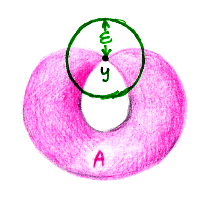
\includegraphics[height=4cm]{bearbeitet-22-04-25/loc0dc.png}
        \caption{Beispiel für eine lokal $0$-dimensional zusammenhängende Raumregion}
        \label{fig:loc0dc}
    \end{figure}
    
    In ähnlicher Weise wird dieser Begriff für Flächenregionen und für lokal $1$-dimensional zusammenhängende Raumregionen definiert.

    \begin{dfn}[Lokal 0/1-zusammenhängend in der \strukt]\ \vspace{0pt}

        \begin{itemize}
            \item Eine Raumregion $A$ ist lokal $0$-dimensional zusammenhängend im Punkt $[A', B', C', \{y\}]$, wenn gilt
            \begin{align*}
                &\Stangpart([A', B', C', \{y\}],A) \land \exists \varepsilon \forall \eta: (\eta < \varepsilon \to 
                \\
                &\SzeroDC(\ball_{\eta}(y) \cap A) \land \neg \SoneDC(\ball_{\eta}(y) \cap A))
            \end{align*}
            \item Eine Flächeregion $[A,B]$ ist lokal $0$-dimensional zusammenhängend im Punkt $[A', B', C', \{y\}]$, wenn gilt
            \begin{align*}
                &\Stangpart([A', B', C', \{y\}],[A,B]) \land \exists \varepsilon \forall \eta:
                %\\
                (\eta < \varepsilon \to
                \\
                &\SzeroDC([A,\ball_{\eta}(y) \cap B]) \land \neg \SoneDC([A,\ball_{\eta}(y) \cap B]))
            \end{align*}
            \item Eine Raumregion $A$ ist lokal $1$-dimensional zusammenhängend im Punkt $[A', B', C', \{y\}]$, wenn gilt
            \begin{align*}
                &\Stangpart([A', B', C', \{y\}],A) \land \exists \varepsilon \forall \eta: (\eta < \varepsilon \to 
                \\
                &\SoneDC(\ball_{\eta}(y) \cap A) \land \neg \StwoDC(\ball_{\eta}(y) \cap A))
            \end{align*}
        \end{itemize}
        
    \end{dfn}
%     
%     In Abbildung \ref{fig:lok0dc} ist ein Beispiel einer lokal 0-dimensional zusammenhängenden Raumregion dargestellt.
%     


    Da es in $\theoryBS$ keinen Abstandsbegriff gibt, lässt sich diese Definition nicht so ohne weiteres auf die Theorie hochziehen. 
    In $\theoryBS$ definiere ich den lokalen Zusammenhang auf folgende Weise:

    % Wenn wir erst den Begriff des maximaldimensionalen zusammenhangs einführen, müssen wir dafür nicht zwischen Raum- und Flächenregionen unterscheiden.
    % 
    % Eine Raumentität ist maximaldimensional zusammenhängend, wenn sie aufgrund ihrer Dimension nicht stärker zusammenhängend sein kann.
    % 
    % \begin{dfn}[$x$ ist maximaldimensional zusammenhängend]
    %     \begin{align*}
    %         \Gmaxcon(x) := 
    %             &(\GSReg(x) \wedge \GtwoDC(x)) \lor 
    %             (\GtwoDE(x) \land \GoneDC(x)) \lor
    %             \\
    %             &(\GoneDE(x) \land \GzeroDC(x)) \lor \GzeroD(x)
    %     \end{align*}
    % 
    % \end{dfn}


    \begin{dfn}[$x$ ist lokal $0$/$1$-dimensional zusammenhängend in $y$]
        \begin{align*}
            \Gloczerodc(x,y) := &\GzeroD(y) \land \Gtangpart(y,x) \land
                                \\
                                &\exists u\ (\forall v w\ (\Ginpart(y,v) \land \Gspart(v,u) \land
                                \\
                                &\Gintersect(x,v,w) \to \neg \GoneDC(w)))
                                \\
            \Gloconedc(x,y) := &\neg \Gloczerodc(x,y) \land \GzeroD(y) \land \Gtangpart(y,x) \land
                                \\
                                &\exists u\ (\forall v w\ (\Ginpart(y,v) \land \Gspart(v,u) \land
                                \\
                                &\Gintersect(x,v,w) \to \neg \GtwoDC(w)))
        \end{align*}

    \end{dfn}

    Es ist noch zu zeigen, dass beide Definitionen kompatibel sind.
    Abbildung \ref{fig:loc1dc} zeigt ein Beispiel einer lokal $1$-dimensional zusammenhängenden Raumregion.

    \begin{figure}[ht]
            \centering
            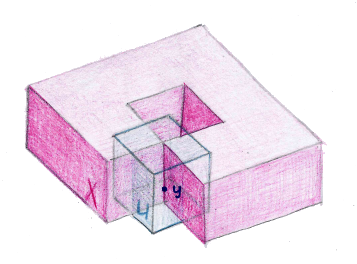
\includegraphics[width=0.6\textwidth]{bearbeitet-22-04-25/loc1dc.png}
            \caption[Beispiel für eine lokal $1$-dimensional zusammenhängende Raumregion]{Beispiel für eine lokal $1$-dimensional zusammenhängende Raumregion: $x$ ist lokal $1$-dimensional zusammenhängend in $y$, da es eine Umgebung $u$ von $y$ gibt, der keinen Teil hat, der auch eine Umgebung von $y$ ist und dessen Schnitt mit $x$ $2$-dimensional zusammen hängt.}
            \label{fig:loc1dc}
    \end{figure}


% \small

% \changetext{}{2cm}{-2cm}{}{} % Anpassung der Seitenränder

%% Beweise topologische Grundlagen
\chapter{Beweise}
\section{Zu Kapitel \ref{chap:topologie-grundlagen} (Grundlagen der Topologie)}

\subsection{Zu Abschnitt \ref{sec:allg-top-raeume} (Allgemeine topologische Räume)}

% --- satz:cl --------------------------------------------------------------------

\subsubsection{zu Satz \ref{satz:cl}.\ref{satz:cl.1}}\label{anh:cl.1}
    Zu zeigen ist: 
    \begin{enumerate}
        \item Aus $\mathcal{M}_A^C := \{ U \in \offen \mid U \cap A = \varnothing\}$ und $U_A^C := \bigcup\limits_{U \in \mathcal{M}_A^C} U$ folgt $\cl(A) = X \setminus U_A^C$. \label{anh:cl.1.1}
        \item $A \subseteq \cl(A)$ \label{anh:cl.1.2}
        \item Es gibt keine kleinere in $X$ abgeschlossene Obermenge von $A$ als $\cl(A)$ \label{anh:cl.1.3}
    \end{enumerate}

    \noindent	
    \textbf{Zu \ref{anh:cl.1.1}:}
        \begin{align*}
            \cl(A) &= \{x \in X \mid \forall\: U \in \offen : (\: x \in U \deshalb U \cap A \neq \varnothing \:) \} &\\
            &= \{x \in X \mid \forall\: U \in \offen : (\: U \cap A = \varnothing \deshalb x \notin U \:) \} &\\
            &= \{x \in X \mid \forall\: U \in \mathcal{M}_A^C : x \notin U \} &\\
        %	&= \{x \in X \mid x \notin \bigcup\limits_{U \in \mathcal{M}_A^C} U \} &\\
            &= \{x \in X \mid x \notin U_A^C \} &= X \setminus U_A^C
        \end{align*}

    \noindent	
    \textbf{Zu \ref{anh:cl.1.2}:} 
        Sei $x \in A$. Dann gilt $\forall\: U \in \offen : (\: x \in U \deshalb U \cap A \neq \varnothing \:)$ und somit $x \in \cl(A)$

    \noindent
    \textbf{Zu \ref{anh:cl.1.3}:}
        Sei $V \in \abg$ mit $A \subseteq V$. Sei $W := X \setminus V$. Dann gelten $W \in \offen$ und $W \cap A = \varnothing$. Damit ist $W \in \mathcal{M}_A^C$ und somit $W \subseteq U_A^C$. Also gilt $ V = X \setminus W \supseteq X \setminus U_A^C = \cl(A)$
        

\subsubsection{Zu Satz \ref{satz:cl}.\ref{satz:cl.2}} \label{anh:cl.2}
    Zu Zeigen ist: $\cl(A) = A \cup \rand(A)$.\\

    \noindent
    \textbf{\glqq$\boldsymbol{\subseteq}$\grqq:}

        \begin{longtable}{r c c l}
            & & 1. & Sei $x \in \cl(A)$ \\
            & & 2. & Angen. $x \notin A \cup \rand(A)$ \\
            2 & $\deshalb$ & 3. & $x \notin \rand(A)$ \\
            3 & $\deshalb$ & 4. & $\exists\: U \in \offen : (\: x \in U \:\land\: (\: U \cap A = \varnothing \:\lor\: U \setminus A = \varnothing \:))$ \\
            4 & $\deshalb$ & 5. & Sei $U \in \offen$ mit $x \in U$ und $U \cap A = \varnothing \:\lor\: U \setminus A = \varnothing$ \\
            2 & $\deshalb$ & 6. & $x \notin A$ \\
            5, 6 & $\deshalb$ & 7. & $x \in U \setminus A$ \\
            7 & $\deshalb$ & 9. & $U \cap A = \varnothing$ \\
            1 & $\deshalb$ & 10. & $\forall\: U \in \offen : (\: x \in U \to U \cap A \neq \varnothing \:)$ \\
            10, 5 & $\deshalb$ & 11. & $U \cap A \neq \varnothing$ \\
            9, 10 & $\deshalb$ & 12. & $\lightning$ 
        \end{longtable}	

    \noindent
    \textbf{\glqq$\boldsymbol{\supseteq}$\grqq:}

        \begin{longtable}{r c c l}
            & & 1. & Sei $x \in A \cup \rand(A)$ \\
            & & 2. & Angen. $x \notin \cl(A)$ \\
            2 & $\deshalb$ & 3. & $\exists\: U \in \offen : (\: x \in U \:\land\: U \cap A = \varnothing \:)$ \\
            3 & $\deshalb$ & 4. & Sei $U \in \offen$ mit $x \in U$ und $U \cap A = \varnothing$ \\
            4 & $\deshalb$ & 5. & $x \notin A$ \\
            1, 5 & $\deshalb$ & 6. & $x \in \rand(A)$ \\
            6 & $\deshalb$ & 7. & $\forall\: U \in \offen : (\: x \in U \to U \cap A \neq \varnothing \:\land\: U \setminus A \neq \varnothing \:)$ \\
            7, 4 & $\deshalb$ & 8. & $U \cap A \neq \varnothing$ \\
            4, 8 & $\deshalb$ & 9. & $\lightning$ 
        \end{longtable}	


\subsubsection{Zu Satz \ref{satz:cl}.\ref{satz:cl.3}} 
    Zu zeigen ist: $\cl(A \cap B) \subseteq \cl(A) \cap \cl(B)$ \\
    \begin{align*}
        &cl(A \cap B) \\
        &= \{x \in X \mid \forall\: U \in \offen : (\: x \in U \to U \cap A \cap B \neq \varnothing \:) \}\\
        &= \{x \in X \mid \forall\: U \in \offen : (\: x \in U \to (U \cap A) \cap (U \cap B) \neq \varnothing \:) \}\\
        &\subseteq \{x \in X \mid \forall\: U \in \offen : (\: x \in U \to U \cap A \neq \varnothing \:\land\: U \cap B \neq \varnothing \:) \}\\
        &= \{x \in X \mid \forall\: U \in \offen : \\
        &\hphantom{XXXXXXX} ((\: x \in U \to U \cap A \neq \varnothing \:) \:\land\: (\: x \in U \to U \cap B \neq \varnothing \:)) \}\\
        &= \{x \in X \mid \forall\: U \in \offen : (\: x \in U \to U \cap A \neq \varnothing \:) \:\land\: \\
        &\hphantom{XXXXXXX} \forall\: U \in \offen :  (\: x \in U \to U \cap B \neq \varnothing \:) \}\\
        &= \{x \in X \mid \forall\: U \in \offen : (\: x \in U \to U \cap A \neq \varnothing \:) \} \cap \\
        &\hphantom{XXXXXXX} \{x \in X \mid \forall\: U \in \offen :  (\: x \in U \to U \cap B \neq \varnothing \:) \}\\
        &= \cl(A) \cap \cl(B)
    \end{align*}


\subsubsection{Zu Satz \ref{satz:cl}.\ref{satz:cl.4}}
    Zu Zeigen ist: $\cl(A \cup B) = \cl(A) \cup \cl(B)$.\\

    \noindent
    \textbf{\glqq$\boldsymbol{\subseteq}$\grqq:}\\
        Da ${\cl(A),\cl(B) \in \abg}$ sind, ist auch ${\cl(A) \cup \cl(B) \in \abg}$ (Satz \ref{satz:CX}) und somit ${\cl(\cl(A) \cup \cl(B))= \cl(A) \cup \cl(B)}$ (Korollar \ref{kor:cl}.\ref{kor:cl.3}). Wegen ${A \subseteq \cl(A)}$ und ${B \subseteq \cl(B)}$ (ebenfalls Satz \ref{satz:CX}) gilt dann
        \begin{align*}
            \cl(A \cup B) \subseteq \cl(\cl(A) \cup \cl(B)) = \cl(A) \cup \cl(B).
        \end{align*}

    \noindent
    \textbf{\glqq$\boldsymbol{\supseteq}$\grqq:}

        \begin{longtable}{r c c l}
            & & 1. & Sei $x \in \cl(A) \cup \cl(B)$ \\
            & & 2. & Angen. $x \notin \cl(A \cup B)$ \\
            2 & $\deshalb$ & 3. & $\exists\: U \in \offen : (\: x \in U \:\land\: U \cap (A \cup B) = \varnothing \:)$ \\
            3 & $\deshalb$ & 4. & Sei $U \in \offen$ mit $x \in U$ und $U \cap (A \cup B) = \varnothing$ \\
            4 & $\deshalb$ & 5. & $(U \cap A) \cup (A \cap B) = \varnothing$ \\
            1 & $\deshalb$ & 6. & $x \in \cl(A) \:\lor\: x \in \cl(B)$ \\
            6 & $\deshalb$ & 7. & $\forall\: U \in \offen : (\: x \in U \to U \cap A \neq \varnothing \:) \:\lor\: \forall\: U \in \offen : (\: x \in U \to U \cap B \neq \varnothing \:)$ \\
            7 & $\deshalb$ & 8. & $\forall\: U \in \offen : ((\: x \in U \to U \cap A \neq \varnothing \:) \:\lor\: (\: x \in U \to U \cap B \neq \varnothing \:))$ \\
            8 & $\deshalb$ & 9. & $\forall\: U \in \offen : (\: x \in U \to (\: U \cap A \neq \varnothing \:\lor\: U \cap B \neq \varnothing \:))$ \\
            9, 4 & $\deshalb$ & 10. & $U \cap A \neq \varnothing \:\lor\: U \cap B \neq \varnothing$ \\
            10 & $\deshalb$ & 11. & $(U \cap A) \cup (U \cap B) \neq \varnothing$ \\
            5, 11 & $\deshalb$ & 12. & $\lightning$ 
        \end{longtable}	
        
        
\subsubsection{Zu Satz \ref{satz:cl}.\ref{satz:cl.5}} 
    Zu zeigen ist: $\cl(X \setminus A) = X \setminus \op(A)$ \\
    \begin{align*}
        \cl(X \setminus A)
        &= \{x \in X \mid \forall\: U \in \offen(x) : U \setminus A \neq \varnothing \}\\
        &= \{x \in X \mid \forall\: U \in \offen(x) : U \nsubseteq A \}\\
        &= \{x \in X \mid \neg \exists\: U \in \offen(x) : U \subseteq A \}\\
        &= X \setminus \op(A)
    \end{align*}


\subsubsection{Zu Satz \ref{satz:cl}.\ref{satz:cl.6}}
    Zu Zeigen ist: $\cl(A \setminus B) \subseteq \cl(A) \setminus \op(B)$.\\

    \begin{longtable}{r c c l}
        & & 1. & Sei $x \in \cl(A \setminus B)$ \\
        1. & $\deshalb$ & 2. & $\forall\: U \in \offen : (\: x \in U \to U \cap (A \setminus B) \neq \varnothing \:)$ \\
        2 & $\deshalb$ & 3. & $\forall\: U \in \offen : (\: x \in U \to (U \cap A) \cap (U \setminus B) \neq \varnothing \:)$ \\
        3 & $\deshalb$ & 4. & $\forall\: U \in \offen : (\: x \in U \to (U \cap A) \neq \varnothing \:\land\: (U \setminus B) \neq \varnothing \:)$ \\
        4 & $\deshalb$ & 5. & $\forall\: U \in \offen : ( (\: x \in U \to U \cap A \neq \varnothing \:) \:\land\: (\: x \in U \to U \setminus B \neq \varnothing \:))$ \\
        5 & $\deshalb$ & 6. & $\forall\: U \in \offen : (\: x \in U \to U \cap A \neq \varnothing \:) \:\land\: \forall\: U \in \offen : (\: x \in U \to U \setminus B \neq \varnothing \:)$ \\
        6 & $\deshalb$ & 7. & $x \in \cl(A)$ und $\neg \exists\: U \in \offen : (\: x \in U \:\land\: U \setminus B = \varnothing \:)$ \\
        7 & $\deshalb$ & 8. & $x \in \cl(A)$ und $\neg \exists\: U \in \offen : (\: x \in U \:\land\: U \subseteq B \:)$ \\
        8 & $\deshalb$ & 9. & $x \in \cl(A)$ und $x \notin \op(B)$ \\
        9 & $\deshalb$ & 10. & $x \in \cl(A) \setminus \op(B)$ \\
    \end{longtable}


\subsubsection{Zu Satz \ref{satz:cl}.\ref{satz:cl.7}} 
    Zu zeigen ist: $\cl(A) \setminus \cl(B) \subseteq \cl(A \setminus B)$

    \begin{longtable}{r c c l}
        & & 1. & Sei $x \in \cl(A) \setminus \cl(B)$ \\
        & & 2. & Angen. $x \notin \cl(A \setminus B)$ \\
        2 & $\deshalb$ & 3. & $\exists\: U \in \offen : (\: x \in U \:\land\: U \cap (A \setminus B) = \varnothing \:)$ \\
        3 & $\deshalb$ & 4. & Sei $U_0 \in \offen$ mit $x \in U_0$ und $U_0 \cap (A \setminus B) = \varnothing$ \\
        1 & $\deshalb$ & 5. & $x \notin \cl(B)$ \\
        5 & $\deshalb$ & 6. & $\exists\: U \in \offen : (\: x \in U \:\land\: U \cap B = \varnothing \:)$ \\
        6 & $\deshalb$ & 7. & Sei $U_1 \in \offen$ mit $x \in U_1$ und $U_1 \cap B = \varnothing$ \\
        1 & $\deshalb$ & 8. & $\forall\: U \in \offen : (\: x \in U \to U \cap A \neq \varnothing \:)$ \\
        4, 7 & $\deshalb$ & 9. & Sei $U_2 := U_0 \cap U_1$ \\
        9, 4, 7 & $\deshalb$ & 10. & $x \in U_2 \in \offen$ \\
        10, 8 & $\deshalb$ & 11. & $U_2 \cap A \neq \varnothing$ \\
        11 & $\deshalb$ & 12. & Sei $y \in U_2 \cap A$ \\
        12 & $\deshalb$ & 13. & $y \in U_2$ \\
        13, 9 & $\deshalb$ & 14. & $y \in U_1$ \\
        14, 7 & $\deshalb$ & 15. & $y \notin B$ \\
        12 & $\deshalb$ & 16. & $y \in A$ \\
        16, 15 & $\deshalb$ & 17. & $y \in A \setminus B$ \\
        13, 9 & $\deshalb$ & 18. & $y \in U_0$ \\
        18, 17 & $\deshalb$ & 19. & $y \in U_0 \cap (A \setminus B)$ \\
        19, 4 & $\deshalb$ & 20. & $\lightning$
    \end{longtable}


\subsubsection{Zu Satz \ref{satz:cl}.\ref{satz:cl.8}} \label{anh:cl.8}
    Zu zeigen: Aus ${A \subseteq B}$ folgt ${\cl(A) \subseteq \cl(B)}$.\\
    Gelte ${A \subseteq B}$ und sei ${x \notin \cl(B)}$. Dann gibt es ein ${U \in \offen}$ mit ${x \in U}$ und ${U \cap B = \varnothing}$. Da für so ein $U$ gilt ${U \cap A \subseteq U \cap B}$, ist dann natürlich auch ${U \cap A = \varnothing}$. Somit gilt: ${\exists\: U \in \offen : (\: x \in U \:\land\: U \cap A = \varnothing \:)}$. Also ist ${x \notin \cl(A)}$.

    
% --- satz:op -----------------------------------------------------------------

\subsubsection{Zu Satz \ref{satz:op}.\ref{satz:op.2}}\label{anh:op.2}
    Zu zeigen ist: $\op(A) = A \setminus \rand(A)$.\\

    \noindent
    \textbf{\glqq$\boldsymbol{\subseteq}$\grqq:}

        \begin{longtable}{r c c l}
            & & 1. & Sei $x \in \op(A)$ \\
            & & 2. & Angen. $x \notin A \setminus \rand(A)$ \\
            1 & $\deshalb$ & 3. & $\exists\: U \in \offen : (\: x \in U \:\land\: U \subseteq A \:)$ \\
            3 & $\deshalb$ & 4. & Sei $U \in \offen$ mit $x \in U$ und $U \subseteq A$. \\
            4 & $\deshalb$ & 5. & $x \in A$ \\
            2, 5 & $\deshalb$ & 6. & $x \in \rand(A)$ \\
            6 & $\deshalb$ & 7. & $\forall\: U \in \offen : (\: x \in U \to U \cap A \neq \varnothing \:\land\: U \setminus A \neq \varnothing \:)$ \\
            7, 4 & $\deshalb$ & 8. & $U \setminus A \neq \varnothing$ \\
            4, 8 & $\deshalb$ & 9. & $\lightning$ 
        \end{longtable}	

    \noindent
    \textbf{\glqq$\boldsymbol{\supseteq}$\grqq:}

        \begin{longtable}{r c c l}
            & & 1. & Sei $x \in A \setminus \rand(A)$ \\
            & & 2. & Angen. $x \notin \op(A)$ \\
            1 & $\deshalb$ & 3. & $x \notin \rand(A)$ \\
            3 & $\deshalb$ & 4. & $\exists\: U \in \offen : (\: x \in U \:\land\: (\: U \cap A = \varnothing \:\lor\: U \setminus A = \varnothing \:))$ \\
            4 & $\deshalb$ & 5. & Sei $U \in \offen$ mit $x \in U$ und $U \cap A = \varnothing \:\lor\: U \setminus A = \varnothing$ \\
            2 & $\deshalb$ & 6. & $\forall\: U \in \offen : (\: x \in U \to U \setminus A \neq \varnothing \:)$ \\
            5, 6 & $\deshalb$ & 7. & $U \setminus A \neq \varnothing$ \\
            7, 4 & $\deshalb$ & 8. & $U \cap A = \varnothing$ \\
            1 & $\deshalb$ & 9. & $x \in A$ \\
            5, 9 & $\deshalb$ & 10. & $x \in U \cap A$ \\	
            8, 10 & $\deshalb$ & 12. & $\lightning$ 
        \end{longtable}


\subsubsection{Zum Beweis von Satz \ref{satz:op}.\ref{satz:op.1}}\label{anh:op.1}
    Zu zeigen ist: Aus ${\mathcal{M}_A := \{U \in \offen \mid U \subseteq A\}}$ folgt $\op(A) = \bigcup\limits_{U \in \mathcal{M}_A} U$.\\

    \noindent
    \textbf{"$\boldsymbol{\subseteq}$":} 
    Sei $x \in \op(A)$. Dann gibt es ein ${U \in \offen}$ mit $x \in U$ und ${U \subseteq A}$. Also ist ${U \in \mathcal{M}_A}$ und somit ${x \in U \subseteq \bigcup\limits_{U \in \mathcal{M}_A} U}$.

    \noindent
    \textbf{"$\boldsymbol{\supseteq}$":}
    Sei $x \in \bigcup\limits_{U \in \mathcal{M}_A} U$. Sei $U \in \mathcal{M}_A$ mit $x \in U$. Dann gelten: $U \in \offen$ und $U \subseteq A$. Also ist $x \in \op(A)$.


\subsubsection{Zu Satz \ref{satz:op}.\ref{satz:op.3}}\label{anh:op.3}
    Zu zeigen ist: $\op(A \cap B) = \op(A) \cap \op(B)$.\\

    \noindent
    \textbf{"$\boldsymbol{\subseteq}$":}
        \begin{align*}
            \op(A \cap B) 
            &= \{x \in X \mid \exists\: U \in \offen: (\: x \in U \:\land\: U \subseteq A \cap B \:)\}\\
            &= \{x \in X \mid \exists\: U \in \offen: (\: x \in U \:\land\: U \subseteq A \:\land\: U \subseteq B \:)\}\\
            &\subseteq \{x \in X \mid \exists\: U \in \offen: (\: x \in U \:\land\: U \subseteq A\:) \:\land\: \\
            &\hphantom{XXXXXXX} \exists\: U \in \offen: (\: x \in U \:\land\: U \subseteq B \:)\}\\
            &= \{x \in X \mid \exists\: U \in \offen: (\: x \in U \:\land\: U \subseteq A\:)\} \cap\\
            &\hphantom{XXXXXXX} \{ x \in X \mid \exists\: U \in \offen: (\: x \in U \:\land\: U \subseteq B \:)\}\\
            &= \op(A) \cap \op(B)
        \end{align*}

    \noindent
    \textbf{"$\boldsymbol{\supseteq}$":}
        \begin{longtable}{r c c l}
            & & 1. & Sei $x \in \op(A) \cap \op(B)$ \\
            1 & $\deshalb$ & 2. & $x \in \op(A)$ \\
            2 & $\deshalb$ & 3. & $\exists\: U \in \offen: (\: x \in U \:\land\: U \subseteq A\:)$ \\
            3 & $\deshalb$ & 4. & Sei $U_A \in \offen$ mit $x \in U_A$ und $U_A \subseteq A$ \\
            1 & $\deshalb$ & 5. & $x \in \op(B)$ \\
            5 & $\deshalb$ & 6. & $\exists\: U \in \offen: (\: x \in U \:\land\: U \subseteq B\:)$ \\
            6 & $\deshalb$ & 7. & Sei $U_B \in \offen$ mit $x \in U_B$ und $U_B \subseteq B$ \\
            4, 7 & $\deshalb$ & 8. & Sei $U := U_A \cap U_B$ \\
            4, 7, 8 & $\deshalb$ & 9. & $x \in U$ \\
            4, 7, 8 & $\deshalb$ & 10. & $U \subseteq A \cap B$ \\
            9, 10 & $\deshalb$ & 11. & $x \in \op(A \cap B)$ \\
        \end{longtable}


\subsubsection{Zu Satz \ref{satz:op}.\ref{satz:op.4}}\label{anh:op.4}
    Zu zeigen ist: $\op(A) \cup \op(B) \subseteq \op(A \cup B)$
    \begin{align*}
        &\op(A) \cup \op(B) \\
        &= \{x \in X \mid x \in \op(A) \:\lor\: x \in \op(B)\} \\
        &= \{x \in X \mid \exists\: U \in \offen : (\: x \in U \:\land\: U \subseteq A \:) \:\lor\:\\
        &\hphantom{XXXXXXX} \exists\: U \in \offen : (\: x \in U \:\land\: U \subseteq B \:) \} \\
        &= \{x \in X \mid \exists\: U \in \offen : ((\: x \in U \:\land\: U \subseteq A \:) \:\lor\: (\: x \in U \:\land\: U \subseteq B \:)) \} \\
        &= \{x \in X \mid \exists\: U \in \offen : (\: x \in U \:\land\: (\: U \subseteq A \:\lor\: U \subseteq B \:)) \} \\
        &\subseteq \{x \in X \mid \exists\: U \in \offen : (\: x \in U \:\land\: U \subseteq A \cup B \:) \} \\
        &= \op(A \cup B)
    \end{align*}
    
    
\subsubsection{Zu Satz \ref{satz:op}.\ref{satz:op.5}} 
    Zu zeigen ist: $\op(X \setminus A) = X \setminus \cl(A)$ \\
    \begin{align*}
        \op(X \setminus A)
        &= \{x \in X \mid \exists\: U \in \offen(x) : U \subseteq X \setminus A \}\\
        &= \{x \in X \mid \exists\: U \in \offen(x) : U \cap A = \varnothing\}\\
        &= \{x \in X \mid \neg \forall\: U \in \offen(x) : U \cap A \neq \varnothing \}\\
        &= X \setminus \cl(A)
    \end{align*}


\subsubsection{Zu Satz \ref{satz:op}.\ref{satz:op.6}}\label{anh:op.5}	
    Zu zeigen ist: $\op(A \setminus B) = \op(A) \setminus \cl(B)$\\

    \noindent
    \textbf{"$\boldsymbol{\subseteq}$":}
        \begin{longtable}{r r c r l}
            & & & 1. & Sei $x \in \op(A \setminus B) $ \\
            & & & 2. & Angen. $x \notin \op(A) \setminus \cl(B)$ \\
            & 1 & $\deshalb$ & 3. & $\exists\: U \in \offen : (\: x \in U \:\land\: U \subseteq A \setminus B \:)$ \\
            & 3 & $\deshalb$ & 4. & Sei $U \in \offen$ mit $x \in U$ und $U \subseteq A \setminus B$ \\
            & 4 & $\deshalb$ & 5. & $\varnothing = U \setminus (A \setminus B) = (U \setminus A) \cup (U \cap B)$ \\
            & 5 & $\deshalb$ & 6. & $U \setminus A = \varnothing$ \\
            & 6 & $\deshalb$ & 7. & $U \cap B = \varnothing$ \\
            & 2 & $\deshalb$ & 8. & $x \notin \op(A) \:\lor\: x \in \cl(B)$ \\
            \hline
            Fall 1: & 8 & $\deshalb$ & 1.9. & $x \notin \op(A)$ \\
            & 1.9. & $\deshalb$ & 1.10. & $\neg \exists\: U \in \offen : (\: x \in U \:\land\: U \subseteq A \:)$ \\
            & 1.10 & $\deshalb$ & 1.11. & $\forall\: U \in \offen : (\: x \in U \to U \setminus A \neq \varnothing \:)$ \\
            & 1.11, 4 & $\deshalb$ & 1.12. & $U \setminus A \neq \varnothing$ \\
            & 1.12, 6 & $\deshalb$ & 1.13. & $\lightning$ \\
            \hline
            Fall 2: 
            & 8 & $\deshalb$ & 2.9. & $x \in \cl(B)$ \\
            & 2.9 & $\deshalb$ & 2.10 & $\forall\: U \in \offen : (\: x \in U \to U \cap B \neq \varnothing \:)$ \\
            & 2.10, 4 & $\deshalb$ & 2.11 & $U \cap B \neq \varnothing$ \\
            & 2.11, 7 & $\deshalb$ & 2.12 & $\lightning$ \\
        \end{longtable}

    \noindent
    \textbf{"$\boldsymbol{\supseteq}$":}

        \begin{longtable}{r c c l}
            & & 1. & Sei $x \in \op(A) \setminus \cl(B)$ \\
            & & 2. & Angen. $x \notin \op(A \setminus B))$ \\
            1 & $\deshalb$ & 3. & $x \in \op(A)$ \\
            3 & $\deshalb$ & 4. & $\exists\: U \in \offen : (\: x \in U \:\land\: U \subseteq A \:)$ \\
            4 & $\deshalb$ & 5. & Sei $U_1 \in \offen$ mit $x \in U_1$ und $U_1 \subseteq A$ \\
            1 & $\deshalb$ & 6. & $x \notin \cl(B)$ \\
            6 & $\deshalb$ & 7. & $\exists\: U \in \offen : (\: x \in U \:\land\: U \cap B = \varnothing \:)$ \\
            7 & $\deshalb$ & 8. & Sei $U_2 \in \offen$ mit $x \in U_2$ und $U_2 \cap B = \varnothing$ \\
            8, 5 & $\deshalb$ & 9. & Sei $U_0 := U_1 \cap U_2 \in \offen$ \\
            9, 5, 8 & $\deshalb$ & 10. & $x \in U_0$ \\
            2 & $\deshalb$ & 11. & $\forall\: U \in \offen : (\: U \setminus (A \setminus B) \neq \varnothing \:)$ \\
            11, 9, 10 & $\deshalb$ & 12. & $U_0 \setminus (A \setminus B) \neq \varnothing$ \\
            12 & $\deshalb$ & 13. & Sei $y \in U_0 \setminus (A \setminus B)$ \\
            13 & $\deshalb$ & 14. & $y \in U_0$ \\
            14, 9 & $\deshalb$ & 15. & $y \in U_1$ \\
            15, 5 & $\deshalb$ & 16. & $y \in A$ \\
            14, 9 & $\deshalb$ & 17. & $y \in U_2$ \\
            17, 7 & $\deshalb$ & 18. & $y \notin B$ \\
            16, 18 & $\deshalb$ & 19. & $y \in A \setminus B$ \\
            19, 13 & $\deshalb$ & 20. & $\lightning$ \\
        \end{longtable}
        

% --- satz:rand ---------------------------------------------------------------------

\subsubsection{Zu Satz \ref{satz:rand}.\ref{satz:rand.1}} \label{anh:rand.1}
    Zu zeigen ist: $\rand(\rand(A)) \subseteq \rand(A))$ \\
    Sei $x \in \rand(\rand(A))$. Dann gilt nach Definition des Randoperators (Def \ref{def:rand})
    \begin{align} \label{anh:rand.1.1}
        \forall\: U \in \offen: (\: x \in U \to (\: U \cap \rand(A) \neq \varnothing \:\land\: U \setminus \rand(A) \neq \varnothing \:))
    \end{align}
    Angenommen $x \notin \rand(A)$. %Dann gilt wiederum nach der Definition des Randoperators 	
    \begin{align*} %\label{anh:rand.1.2}
        \exists\: U \in \offen : (\: x \in U \:\land\: (\: U \cap A = \varnothing \:\lor\: U \setminus A = \varnothing \:))
    \end{align*}
    Sei also $U_0 \in \offen$ mit $x \in U_0$ und
    \begin{align} \label{anh:rand.1.3}
        U_0 \cap A = \varnothing \:\lor\: U_0 \setminus A = \varnothing
    \end{align}
    nach (\ref{anh:rand.1.1}) gilt jetzt $U_0 \cap \rand(A) \neq \varnothing$. Sei also $y \in U_0 \cap \rand(A)$.
    %Dann gilt wieder nach Definition des Randoperators
    \begin{align*} %\label{anh:rand.1.4}
        \forall\: U \in \offen: (\: y \in U \to (\: U \cap A \neq \varnothing \:\land\: U \setminus A \neq \varnothing))
    \end{align*}
    Also
    \begin{align*}
        U_0 \cap A \neq \varnothing \:\land\: U_0 \setminus A \neq \varnothing
    \end{align*}
    was (\ref{anh:rand.1.3}) widerspricht.

	
\subsubsection{Zu Satz \ref{satz:rand}.\ref{satz:rand.2}}\label{anh:rand.2}
    Zu zeigen ist: $\rand(A) = \cl(A) \setminus \op(A)$
    \begin{align*}
    \cl(A) \setminus \op(A) &= &&\cl(A) \cap (X \setminus \op(A))\\
                            &= &&\{x \in X \mid \forall\: U \in \offen: (\: x \in U \to U \cap A \neq \varnothing \:)\}\\ 
                            &  &&\cap \{x \in X \mid \neg \exists\: U \in \offen: (\: x \in U \:\land\: U \subseteq A\:)\}\\
                            &= &&\{x \in X \mid \forall\: U \in \offen: (\: x \in U \to U \cap A \neq \varnothing\:) \:\land\:\\ 
                            &  &&\forall\: U \in \offen:(\: x \in U \to \neg(U \subseteq A) \:) \}\\
                            &= &&\{x \in X \mid \forall\: U \in \offen: (\: (\: x \in U \to U \cap A \neq \varnothing \:) \:\land\:\\
                            &  &&(\: x \in U \to U \setminus A \neq \varnothing \:) \:) \}\\
                            &= &&\{x \in X \mid \forall\: U \in \offen: (\: x \in U \to (\: U \cap A \neq \varnothing \:\land\: U \setminus A \neq \varnothing \:) \:) \}\\
                            &= &&\rand(A)
    \end{align*}


\subsubsection{Zu Satz \ref{satz:rand}.\ref{satz:rand.3}}\label{anh:rand.3}
    Zu zeigen ist: $(\rand(A) \cap \op(B)) \cup (\rand(B) \cap \op(A)) \subseteq \rand(A \cap B)$.\\ \ \\
    Ich zeige:
    \begin{enumerate}
    \item\label{anh:rand.3.1} $\rand(A) \cap \op(B) \subseteq \rand(A \cap B) \quad$ und
    \item\label{anh:rand.3.2} $\rand(B) \cap \op(A) \subseteq \rand(A \cap B)$
    \end{enumerate}

    \noindent
    \textbf{Zu \ref{anh:rand.3.1}: }
        \begin{longtable}{r c r l}
                    &          &  1. & Sei $x \in \rand(A) \cap \op(B)$ \\
                    &          &  2. & Angen. $x \notin \rand(A \cap B)$ \\
            1          & $\deshalb$ &  3. & $x \in \op(B)$ \\
            3          & $\deshalb$ &  4. & $\exists\: U \in \offen: (\: x \in U \:\land\: U \subseteq B \:) $ \\
            4          & $\deshalb$ &  5. & Sei $U_1 \in \offen$ mit $x \in U_1$ und $U_1 \subseteq B$ \\
            2          & $\deshalb$ &  6. & $\exists\: U \in \offen: (\: x \in U \:\land\: (\: U \cap A \cap B = \varnothing \:\lor\: U \setminus (A \cap B) = \varnothing \:) \:)$ \\
            6          & $\deshalb$ &  7. & Sei $U_2 \in \offen$ mit $x \in U_2$ und $U_2 \cap A \cap B = \varnothing \:\lor\: U_2 \setminus (A \cap B) = \varnothing$ \\
            5, 7       & $\deshalb$ &  8. & Sei $U := U_1 \cap U_2$ \\
            5, 7, 8    & $\deshalb$ &  9. & $x \in U \in \offen$ \\
            1          & $\deshalb$ & 10. & $x \in \rand(A)$ \\
            10         & $\deshalb$ & 11. & $\forall\: U \in \offen: (\: x \in U \to (\: U \cap A \neq \varnothing \:\land\: U \setminus A \neq \varnothing \:) \:) $ \\
            9, 11      & $\deshalb$ & 12. & $U \cap A \neq \varnothing \:\land\: U \setminus A \neq \varnothing$ \\
            12         & $\deshalb$ & 13. & Sei $y \in U \setminus A$ \\
            13, 8      & $\deshalb$ & 14. & $y \in U_2$ \\
            13         & $\deshalb$ & 15. & $y \notin A \supseteq A \cap B$ \\
            14, 15     & $\deshalb$ & 16. & $y \in U_2 \setminus (A \cap B)$ \\
            7, 16      & $\deshalb$ & 17. & $U_2 \cap A \cap B = \varnothing$ \\
            11         & $\deshalb$ & 18. & Sei $z \in U \cap A$ \\
            8, 18      & $\deshalb$ & 19. & $z \in U_1$ \\
            5, 19      & $\deshalb$ & 20. & $z \in B$ \\
            8, 18      & $\deshalb$ & 21. & $z \in U_2$ \\
            18, 20, 21 & $\deshalb$ & 22. & $z \in U_2 \cap A \cap B$ \\
            17, 22     & $\deshalb$ & 23. & $\lightning$
        \end{longtable}

    \noindent
    \textbf{Zu \ref{anh:rand.3.1}: } analog

\subsubsection{Zu Satz \ref{satz:rand}.\ref{satz:rand.4}}\label{anh:rand.4}
    Zu zeigen ist: $\rand(A \cap B) \subseteq (\rand(A) \cap \cl(B)) \cup (\rand(B) \cap \cl(A))$.\\ \ \\

    \noindent
    \textbf{Vorüberlegung (*): } Für beliebige $A, B \subseteq X$ gilt:
        \begin{align*}
            &\rand(A) \cap \cl(B) \\ 
            &= \{x \in X \mid \forall\: U \in \offen: (\: x \in U \to (\: U \cap A \neq \varnothing \:\land\: U \setminus A \neq \varnothing \:) \:)\}\\
            &\hphantom{XXXXXXX}\cap \{x \in X \mid \forall\: U \in \offen: (\: x \in U \to U \cap B \neq \varnothing \:)\}\\
            &= \{x \in X \mid \forall\: U \in \offen: (\: x \in U \to (\: U \cap A \neq \varnothing \:\land\:\\
            &\hphantom{XXXXXXX} U \setminus A \neq \varnothing \:\land\: U \cap B \neq \varnothing \:) \:)\}
        \end{align*}

    \begin{longtable}{r c r l}
        & & 1. & Sei $x \in \rand(A \cap B)$ \\
        & & 2. & Angen. $x \notin (\rand(A) \cap \cl(B)) \cup (\rand(B) \cap \cl(A))$ \\
        2 & $\deshalb$ & 3. & $x \notin \rand(A) \cap \cl(B)$ \\
        3, * & $\deshalb$ & 4. & $\exists\: U \in \offen: (\: x \in U \:\land\:$\\
                             &&& $(\: U \cap A = \varnothing \:\lor\: U \setminus A = \varnothing \:\lor\: U \cap B = \varnothing \:) \:) $ \\
        4 & $\deshalb$ & 5. & Sei $U_1 \in \offen$ mit $x \in U_1$ und\\
                              &&& $U_1 \cap A = \varnothing \:\lor\: U_1 \setminus A = \varnothing \:\lor\: U_1 \cap B = \varnothing$ \\
        2 & $\deshalb$ & 6. & $x \notin \rand(B) \cap \cl(A)$ \\
        6, * & $\deshalb$ & 7. & $\exists\: U \in \offen: (\: x \in U \:\land\:$\\
                             &&& $(\: U \cap B = \varnothing \:\lor\: U \setminus B = \varnothing \:\lor\: U \cap A = \varnothing \:) \:)$ \\
        7 & $\deshalb$ & 8. & Sei $U_2 \in \offen$ mit $x \in U_2$ und\\
                          &&& $U_2 \cap B = \varnothing \:\lor\: U_2 \setminus B = \varnothing \:\lor\: U_2 \cap A = \varnothing$\\
        5, 8 & $\deshalb$ & 9. & Sei $U := U_1 \cap U_2$ \\
        1 & $\deshalb$ & 10. & $\forall\: U \in \offen: (\: x \in U \to$\\
                           &&& $U \cap A \cap B \neq \varnothing \:\land\: U \setminus (A \cap B) \neq \varnothing \:) \:) $ \\
        5, 8, 9 & $\deshalb$ & 11. & $x \in U \in \offen$ \\
        10, 11 & $\deshalb$ & 12. & $U \cap A \cap B \neq \varnothing$ und $U \setminus (A \cap B) \neq \varnothing$ \\
        9, 12 & $\deshalb$ & 13. & $U_1 \cap U_2 \cap A \cap B \neq \varnothing$ \\
        13 & $\deshalb$ & 14. & $U_1 \cap A \neq \varnothing$ \\
        13 & $\deshalb$ & 15. & $U_1 \cap B \neq \varnothing$ \\
        5, 14, 15 & $\deshalb$ & 16. & $U_1 \setminus A = \varnothing$ \\
        9, 16 & $\deshalb$ & 17. & $U \setminus A = (U_1 \cap U_2) \setminus A \subseteq U_1 \setminus A = \varnothing$ \\
        13 & $\deshalb$ & 18. & $U_2 \cap A \neq \varnothing$ \\
        13 & $\deshalb$ & 19. & $U_2 \cap B \neq \varnothing$ \\
        8, 18, 19 & $\deshalb$ & 20. & $U_2 \setminus B = \varnothing$ \\
        9, 20 & $\deshalb$ & 21. & $U \setminus B = (U_1 \cap U_2) \setminus B \subseteq U_2 \setminus B = \varnothing $ \\
        17, 21 & $\deshalb$ & 22. & $\varnothing = (U \setminus A) \cup (U \setminus B) = U \setminus (A \cap B) $ \\
        12, 22 & $\deshalb$ & 23. & $\lightning$
    \end{longtable}


\subsubsection{Zu Satz \ref{satz:rand}.\ref{satz:rand.7}}\label{anh:rand.7}
    Zu zeigen ist: $\rand(A \setminus B) \subseteq (\rand(A) \setminus \op(B)) \cup (\rand(B) \cap \cl(A))$

    \begin{longtable}{r r c r l}
        & & & 1. & Sei $x \in \rand(A \setminus B) $ \\
        & & & 2. & Angen. $x \notin (\rand(A) \setminus \op(B)) \cup (\rand(B) \cap \cl(A))$ \\
        & 1 & $\deshalb$ & 3. & $\forall\: U \in \offen : (\: x \in U \to$\\
                           &&&& $(\: U \cap (A \setminus B) \neq \varnothing \:\land\: U \setminus (A \setminus B) \neq \varnothing \:))$ \\
        & 2 & $\deshalb$ & 4. & $x \notin \rand(A) \setminus \op(B)$ \\
        & 4 & $\deshalb$ & 5. & $x \notin \rand(A) \:\lor\: x \in \op(B)$ \\
        \hline
        Fall 1: & & & 1.1. & $x \in \op(B)$ \\
        &  & $\deshalb$ & 1.2. & $\exists\: U \in \offen : (\: x \in U \:\land\: U \subseteq B \:)$ \\
        & 1.2 & $\deshalb$ & 1.3. & Sei $U \in \offen$ mit $x \in U$ und $U \subseteq B$  \\
        & 3, 1.3 & $\deshalb$ & 1.4. & $U \cap (A \setminus B) \neq \varnothing$ \\
        & 1.4 & $\deshalb$ & 1.5. & $U \setminus B \neq \varnothing$ \\
        & 1.5, 1.3 & $\deshalb$ & 1.6. & $\lightning$ \\
        \hline
        Fall 2: & & & 2.1. & $x \notin \op(B)$ \\
        & 5, 2.1 & $\deshalb$ & 2.2. & $x \notin \rand(A)$ \\
        & 2.2 & $\deshalb$ & 2.3. & $\exists\: U \in \offen : (\: x \in U \:\land\: (\: U \cap A = \varnothing \:\lor\: U \setminus A = \varnothing \:))$ \\
        & 2.3 & $\deshalb$ & 2.4. & Sei $U_0 \in \offen$ mit $x \in U_0$ und\\
                               &&&& $U_0 \cap A = \varnothing \:\lor\: U_0 \setminus A = \varnothing$ \\
        & 3, 2.4 & $\deshalb$ & 2.5. & $U_0 \cap (A \setminus B) \neq \varnothing$ \\
        & 2.5 & $\deshalb$ & 2.6. & $U_0 \cap A \neq \varnothing$ \\
        & 2.6, 2.4 & $\deshalb$ & 2.7. & $U_0 \setminus A = \varnothing$ \\
        & 2.4, 2.7 & $\deshalb$ & 2.8. & $x \in A$ \\
        & 2.8 & $\deshalb$ & 2.9. & $x \in \cl(A)$ \\
        & 2 & $\deshalb$ & 2.10. & $x \notin \rand(B) \cap \cl(A)$ \\
        & 2.10, 2.9 & $\deshalb$ & 2.11. & $x \notin \rand(B)$ \\
        & 2.11 & $\deshalb$ & 2.12. & $\exists\: U \in \offen : (\: x \in U \:\land\: (\: U \cap B = \varnothing \:\lor\: U \setminus B = \varnothing \:))$ \\
        & 2.12 & $\deshalb$ & 2.13. & Sei $U_1 \in \offen$ mit $x \in U_1$ und\\
                                 &&&& $U_1 \cap B = \varnothing \:\lor\: U_1 \setminus B = \varnothing$ \\
        & 2.11, 2.1 & $\deshalb$ & 2.14. & $x \notin \cl(B) \subseteq B$ \\
        & 2.13, 2.14 & $\deshalb$ & 2.15. & $x \in U_1 \setminus B$ \\
        & 2.15 & $\deshalb$ & 2.16. & $U_1 \setminus B \neq \varnothing$ \\
        & 2.16, 2.13 & $\deshalb$ & 2.17. & $U_1 \cap B = \varnothing$ \\
        & 2.13, 2.4 & $\deshalb$ & 2.18. & Sei $U_2 := U_0 \cap U_1 \in \offen$ \\
        & 2.13, 2.4, 2.18 & $\deshalb$ & 2.19. & $x \in U_2$ \\
        & 3, 2.18, 2.19 & $\deshalb$ & 2.20. & $U_2 \setminus (A \setminus B) \neq \varnothing$ \\
        & 2.18 & $\deshalb$ & 2.23. & $U_2 \subseteq U_0$ \\
        & 2.23, 2.7 & $\deshalb$ & 2.24. & $U_2 \setminus A = \varnothing$ \\
        & 2.18 & $\deshalb$ & 2.25. & $U_2 \subseteq U_1$ \\
        & 2.17, 2.25 & $\deshalb$ & 2.26. & $U_2 \cap B = \varnothing$ \\
        & 2.24, 2.26 & $\deshalb$ & 2.27. & $\varnothing = (U_2 \setminus A) \cup (U_2 \cap B)$\\
                                       &&&& $= U_2 \setminus (A \setminus B)$ \\
        & 2.17, 2.20 & $\deshalb$ & 2.28. & $\lightning$ \\
    \end{longtable}
    
    
% --- bsp:standardbsp-rand-hp -----------------------------------------------------

\subsubsection{Zu Bsp.~\ref{bsp:standardbsp-rand-hp}}\label{anh:standardbsp-rand-hp}
    Zu zeigen ist: Für $\rand A = \{\frac{1}{2^n} \mid n \in \N\} \cup \{0\}$ ist $0$ der einzige Häufungspunkt.\\ \ \\
    %
    Sei $x \in \R$.\\ \ \\
        \textbf{Fall 1:} $x < 0$.\\
            Dann ist $U := (2x,\frac{x}{2})$ eine offene Umgebung von $x$ in $\R$ mit $\varnothing = U \cap \rand A \subseteq U \cap (\rand A \setminus \{x\})$.
            Also ist $x$ keine Häufungspunkt von $\rand A$.\\ \ \\
        \textbf{Fall 2:} $x = 0$.\\
            Sei $U \in \offen({0})$. Dann gibt es nach Definition der Standardtopologie ein offenes Intervall $(a,b)$ mit $a < 0 < b$ und $(a,b) \subseteq U$.\\ 
            Sei $N \in \N$ mit $\frac{1}{2^N} < b$. 
            Dann ist $0 \neq N \in \rand A \cap (a,b) \subseteq \rand A \cap U$ und somit $U \cap (\rand A \setminus \{0\}) \neq \varnothing$. 
            Also ist $0 = x$ ein Häufungspunkt von $\rand A$.\\ \ \\
        \textbf{Fall 3:} $0 < x \leq \frac{1}{2}$, $x \in \rand A$.\\
            Sei $N \in \N$ mit $x = 2^{-N}$. Dann ist $(2^{-N-1}, 2^{-N+1})$ eine offene Umgebung von $x$ in $\R$, die nur $x$ als Punkt in $\rand A$ enthält.
            Somit ist $x$ kein Häufungspunkt von $\rand A$.\\ \ \\
        \textbf{Fall 4:} $0 < x \leq \frac{1}{2}$, $x \notin \rand A$.\\
            Sei $N$ die kleinste natürliche Zahlr für die $\frac{1}{2^N} < x$ ist. Dann ist $(2^{-N}, 2^{-N+1})$ eine offene Umgebung von $x$ in $\R$, die keine Randpunkte von $A$ enthält.
            Somit ist $x$ kein Häufungspunkt von $\rand A$.\\ \ \\
        \textbf{Fall 5:} $x > \frac{1}{2}$.\\
            Dann ist $U := (\frac{x}{2}+\frac{1}{4},2x)$ eine offene Umgebung von $x$ in $\R$ mit $\varnothing = U \cap \rand A \subseteq U \cap (\rand A \setminus \{x\})$.
            Also ist $x$ keine Häufungspunkt von $\rand A$.
    

% --- satz:cl-op-hp ---------------------------------------------------------------
    
\subsubsection{Zu Satz \ref{satz:cl-op-hp}}\label{anh:cl-op-hp}
    Zu zeigen sind:
    \begin{enumerate}
        \item \label{anh:cl-op-hp.1} $\cl(A) = A \cup \HP(A)$
        \item \label{anh:cl-op-hp.2} $\op(A) = A \setminus \HP(X \setminus A)$
    \end{enumerate}
    
    \noindent
    \textbf{Zu \ref{anh:cl-op-hp.1}: }\\
    \textbf{``$\boldsymbol{\subseteq}$``:}
        Wenn $x$ nicht aus $A \cup \HP(A)$ ist, dann ist $x \notin \HP(A)$ und somit gibt es ein $U \in \offen(x)$ mit $U \cap (A \setminus \{x\}) = \varnothing$.
        Da $x$auch nicht in $A$ ist, ist $A \setminus \{x\} = A$ und somit $U \cap A = \varnothing$. Also ist $x$ nicht in $\cl(A)$.\\
    \textbf{``$\boldsymbol{\supseteq}$``:}
        Wenn $x$ nicht in $\cl(A)$ ist, dann gibt es ein $U \in \offen(x)$ mit $U \cap A = \varnothing$ und dann ist erst recht $U \cap (A \setminus \{x\}) = \varnothing$. Also ist $x$ kein Häufungspunkt von $A$.\\ \ \\
    
    \noindent
    \textbf{Zu \ref{anh:cl-op-hp.2}: }\\
    \textbf{``$\boldsymbol{\subseteq}$``:}
        Wenn $x$ in $\op(A)$ ist, so gibt es ein $U \in \offen(x)$ mit $U \subseteq A$.
        Dann gilt $U \cap ((X \setminus A) \setminus \{x\}) \subseteq U \cap (X \setminus A) = U \setminus A = \varnothing$.
        Somit ist $x$ kein Häufungspunkt von $X \setminus A$ und da $x \in \op(A) \subseteq A$ ist, ist $x \in A \setminus \HP(X \setminus A)$.\\
    \textbf{``$\boldsymbol{\supseteq}$``:}
        Wenn $x \in A \setminus \HP(X \setminus A)$ ist, so ist $x$ kein Häufungspunkt von $X \setminus A$ und es gibt ein $U \in \offen(x)$ mit $\varnothing = U \cap ((X \setminus A) \setminus \{x\}) = U \setminus (X \setminus (A \cup \{x\}))$ und da $x \in A$ ist, gilt $U \setminus A = U \setminus (A \cup \{x\}) = U \setminus (X \setminus (A \cup \{x\})) = \varnothing$. Somit ist $U \subseteq A$ und $x \in \op(A)$.

    

% --- satz:AdB=AdC ----------------------------------------------------------------

\subsubsection{Zu Satz \ref{satz:AdB=AdC}}\label{anh:AdB=AdC}
    Zu zeigen ist: Aus $A \in \offen_X$ und $A \cap B = A \cap C$ folgt $A \cap \rand_X(B) = A \cap \rand_X(C)$\\

    \noindent
    \textbf{\glqq$\boldsymbol{\subseteq}$\grqq:}

    \begin{longtable}{r c c l}
        & & 1. & Sei $A \in \offen_X$ \\
        & & 2. & Gelte $A \cap B = A \cap C$ \\
        & & 3. & Sei $x \in A \cap \rand_X(B)$ \\
        & & 4. & Angen. $x \notin A \cap \rand_X(C)$ \\
        3 & $\deshalb$ & 5. & $x \in A$ \\
        4, 5 & $\deshalb$ & 6. & $x \notin \rand_X(C)$ \\
        6 & $\deshalb$ & 7. & $\exists\: U \in \offen_X (\: x \in U \:\land\: (\: U \cap C = \varnothing \:\lor\: U \setminus C = \varnothing \:))$ \\
        7 & $\deshalb$ & 8. & Sei $U_0 \in \offen_X$ mit $x \in U_0$ und $U_0 \cap C = \varnothing \:\lor\: U_0 \setminus C = \varnothing$ \\
        1, 8 & $\deshalb$ & 9. & Sei $U_1 := U_0 \cap A$ \\
        1, 8, 9 & $\deshalb$ & 10. & $U_1 \in \offen_X$ \\
        3, 8, 9 & $\deshalb$ & 11. & $x \in U_1$ \\
        2 & $\deshalb$ & 12. & $x \in \rand_X(B)$ \\
        12 & $\deshalb$ & 13. & $\forall\: U \in \offen (\: x \in U \to U \cap B \neq \varnothing \:\land\: U \setminus B \neq \varnothing \:)$ \\
        10, 11, 13 & $\deshalb$ & 14. & $U_1 \cap B \neq \varnothing \:\land\: U_1 \setminus B \neq \varnothing$ \\
        9, 2 & $\deshalb$ & 15. & $U_1 \cap B = U_0 \cap A \cap B = U_0 \cap A \cap C = U_1 \cap C$ \\
        9, 2 & $\deshalb$ & 16. & $U_1 \setminus B = U_1 \setminus (U_1 \cap B) = U_1 \setminus (U_0 \cap A \cap B)$ \\
        & & & $= U_1 \setminus (U_0 \cap A \cap C) = U_1 \setminus (U_1 \cap C) = U_1 \setminus C $ \\
        14, 15, 16 & $\deshalb$ & 17. & $U_1 \cap C \neq \varnothing \:\land\: U_1 \setminus C \neq \varnothing$ \\ 
        9 & $\deshalb$ & 18. & $U_1 \subseteq U_0$ \\
        17, 18 & $\deshalb$ & 19. & $U_0 \cap C \neq \varnothing \:\land\: U_0 \setminus C \neq \varnothing$ \\
        8, 19 & $\deshalb$ & 20. & $\lightning$ 
    \end{longtable}

    \noindent
    \textbf{\glqq$\boldsymbol{\supseteq}$\grqq:} analog
    
    
    
    
%%%%%%%%%%%%%%%%%%%%%%%%%%%%%%%%%%%%%%%%%%%%%%%%%%%%%%%%%%%%%%%%%%%%
%%%%%%%%%%%%%%%%%%%%%%%%%%%%%%%%%%%%%%%%%%%%%%%%%%%%%%%%%%%%%%%%%%%%
%%%%%%%%%%%%%%%%%%%%%%%%%%%%%%%%%%%%%%%%%%%%%%%%%%%%%%%%%%%%%%%%%%%%





\subsection{Zu Abschnitt \ref{sec:teilraum-top} (Teilraumtopologie)}


% --- satz:trAbg ------------------------------------------------------------------

\subsubsection{Zu Satz \ref{satz:trAbg}}\label{anh:trAbg}
Zu zeigen ist
\begin{enumerate}
	\item $B \in \abg_A \Rightarrow \exists\: B' \in \abg_X : B = B' \cap A$ \label{anh:trAbg.1}
	\item $\exists\: B' \in \abg_X : B = B' \cap A \Rightarrow B \in \abg_A$ \label{anh:trAbg.2}
\end{enumerate}

\noindent
\textbf{Zu \ref{anh:trAbg.1}:} \\
Sei $B \in C_A$. Dann gibt es ein $C \in \offen_A$ mit $B = A \setminus C$. Dann gibt es ein $D \in \offen$ mit $C = D \cap A$. Sei $B' := X \setminus D$. Dann gelten 
\begin{align*}
	&B' \in \abg_X \quad \textnormal{und} \\
	&B' \cap A = (X \setminus D) \cap A = (X \cap A) \setminus (D \cap A) = A \setminus C = B
\end{align*}

\noindent
\textbf{Zu \ref{anh:trAbg.2}:} \\
Sei $B' \in \abg_X$ mit $B = B' \cap A$. Dann ist $X \setminus B' \in \offen_X$ und damit 
\begin{align*}
	A \setminus B = (X \cap A) \setminus (B' \cap A) =(X \setminus B') \cap A \in \offen_A.
\end{align*}
Also ist $B \in \abg_A$. \\


% --- satz:dAB<clB -----------------------------------------------------------------
	
\subsubsection{Zu Satz \ref{satz:dAB<clB}}\label{anh:dAB<clB}
Zu zeigen ist: $\rand_A(B) \subseteq \cl_X(B)$
\\

\begin{longtable}{r c c l}
	& & 1. & Sei $x \in \rand_A(B)$ \\
	& & 2. & Angen. $x \notin \cl_X(B)$ \\
	2 & $\deshalb$ & 3. & $\exists\: U \in \offen_X : (\: x \in U \:\land\: U \cap B = \varnothing$ \\
	3 & $\deshalb$ & 4. & Sei $U_0 \in \offen_X$ mit $x \in U_0$ und $U_0 \cap B = \varnothing$ \\
	4 & $\deshalb$ & 5. & $U_0 \cap A \in \offen_A$ \\
	6 & $\deshalb$ & 6. & $x \in A$ \\
	4, 6 & $\deshalb$ & 7. & $x \in U_0 \cap A$ \\
	1 & $\deshalb$ & 8. & $\forall\: V \in \offen_A : (\: x \in V \to V \cap B \neq \varnothing \:\land\: V \setminus B \neq \varnothing \:)$ \\
	4, 7, 8 & $\deshalb$ & 9. & $U_0 \cap A \cap B \neq \varnothing$ \\
	9 & $\deshalb$ & 10. & $U_0 \cap B \neq \varnothing$ \\
	4, 10 & $\deshalb$ & 11. & $\lightning$ \\
\end{longtable}


% --- satz:clA1-teil-clA2 -----------------------------------------------

\subsubsection{Zu Satz \ref{satz:clA1-teil-clA2}}\label{anh:clA1-teil-clA2}
    Zu zeigen ist: Aus ${B \subseteq A_1 \cap A_2}$ und ${\cl_{A_1}(B) \subseteq A_2}$ folgt ${\cl_{A_1}(B) \subseteq \cl_{A_2}(B)}$.
    %
    \begin{longtable}{r c c l}
        & & 1. & Sei $x \in \cl_{A_1}(B) \subseteq A_2$ \\
        & & 2. & Angen. $x \notin \cl_{A_2}(B))$ \\
        1 & $\deshalb$ & 3. & $\exists\: V \in \offen_{A_2}(x) : V \cap B = \varnothing$\\
        3 & $\deshalb$ & 4. & Sei $V_2 \in \offen_{A_2}(x)$ mit $V_2 \cap B = \varnothing$ \\
        4 & $\deshalb$ & 5. & Sei $U \in \offen_X$ mit $V_2 = U \cap A_2$ \\
        5 & $\deshalb$ & 6. & Sei $V_1 := U \cap A_1$ \\
        4, 5 & $\deshalb$ & 7. & $x \in U$ \\
        1 & $\deshalb$ & 8. & $x \in A_1$ \\
        7, 8 & $\deshalb$ & 9. & $x \in V_1 \in \offen_{A_1}$ \\
        1 & $\deshalb$ & 10. & $\forall\: V \in \offen_{A_1}(x): V \cap B \neq \varnothing$ \\
        9, 10 & $\deshalb$ & 11. & $V_1 \cap B \neq \varnothing$ \\
        4, 11, $B \subseteq A_2$ & $\to$ & 12. & $\varnothing \neq V_1 \cap B \subseteq U \cap A_2 \cap B = V_2 \cap B = \varnothing$ \\
        12 & $\deshalb$ & 13. & $\lightning$
    \end{longtable}

% --- satz:cl-dA1-dA2 ---------------------------------------------------

\subsubsection{Zu Satz \ref{satz:cl-dA1-dA2}}\label{anh:cl-dA1-dA2}
    Zu zeigen ist: Aus $B \subseteq \rand A_1 \cap \rand A_2$ folgt $\cl_{\rand A_1}(B) \subseteq \rand A_2$

    \begin{longtable}{r c c l}
        & & 0. & $B \subseteq \rand A_1 \cap \rand A_2$\\
        & & 1. & $x \in \cl_{\rand A_1}(B)$ \\
        & & 2. & Angen. $x \notin \rand A_2$ \\
        2 & $\deshalb$ & 3. & $\exists\: U \in \offen_X(x) : (\: U \cap A_2 = \varnothing \:\lor\: U \setminus A_2 = \varnothing \:)$ \\
        3 & $\deshalb$ & 4. & Sei $U \in \offen(x)$ mit $U \cap A_2 = \varnothing$ oder $U \setminus A_2 = \varnothing$ \\
        4 & $\deshalb$ & 5. & Sei $V := U \cap \rand A_1 \in \offen_{\rand A_1}$ \\
        1 & $\deshalb$ & 6. & $x \in \rand A_1$ \\
        5, 6 & $\deshalb$ & 7. & $V \in \offen_{\rand A_1}(x)$ \\
        1 & $\deshalb$ & 8. & $\forall\: V \in \offen_{\rand A_1}: V \cap B \neq \varnothing$ \\
        8 & $\deshalb$ & 9. & $V \cap B \neq \varnothing$ \\
        0, 5, 9 & $\deshalb$ & 10. & Sei $y \in V \cap B \subseteq U \cap \rand A_2$ \\
        10 & $\deshalb$ & 11. & $U \in \offen(y)$ \\
        10 & $\deshalb$ & 12. & $y \in \rand A_2$ \\
        12 & $\deshalb$ & 13. & $\forall\: U \in \offen(y) : (\: U \cap A_2 \neq \varnothing \:\land\: U \setminus A_2 \neq \varnothing \:)$ \\
        11, 13 & $\deshalb$ & 14. & $U \cap A_2 \neq \varnothing \:\land\: U \setminus A_2 \neq \varnothing$ \\
        3, 14 & $\deshalb$ & 15. & $\lightning$
    \end{longtable}
    
    

% --- satz:cl-rand-A1-A2 ----------------------------------------------------
%\subsubsection{Zu Satz \ref{satz:cl-rand-A1-A2}}\label{anh:cl-rand-A1-A2}
%    Zu zeigen ist: Aus ${B \subseteq \rand A_1 \cap \rand A_2}$ folgt ${\cl_{\rand A_1}(B) = \cl_{\rand A_2}(B)}$.\\ \ \\
    %
%    \glqq $\boldsymbol{\subseteq}$\grqq :
    %
%    \begin{longtable}{r c c l}
%        & & 0. & $B \subseteq \rand A_1 \cap \rand A_2$\\
%        & & 1. & Sei $x \in \cl_{\rand A_1}(B)$ \\
%        & & 2. & Angen. $x \notin \cl_{\rand A_2}(B))$ \\
%        0, 1, \ref{satz:cl-dA1-dA2} & $\to$ & 3. & $x \in \rand A_2$\\
%        2, 3 & $\deshalb$ & 4. & $\exists\: V \in \offen_{\rand A_2}(x) : V \cap B = \varnothing$ \\
%        4 & $\deshalb$ & 5. & Sei $V_2 \in \offen_{\rand A_2}(x)$ mit $V_2 \cap B = \varnothing$ \\
%        5 & $\deshalb$ & 6. & $\exists\: U \in \offen: V = U \cap \rand A_2$ \\
%        6 & $\deshalb$ & 7. & Sei $U \in \offen$ mit $V = U \cap \rand A_2$ \\
%        7 & $\deshalb$ & 8. & Sei $V_1 := U \cap \rand A_1 \in \offen_{\rand A_1}$ \\
%        5, 7 & $\deshalb$ & 9. & $x \in V_2 \subseteq U$ \\
%        1 & $\deshalb$ & 10. & $x \in \rand A_1$ \\
%        9, 10 & $\deshalb$ & 11. & $x \in V_1 \in \offen_{\rand A_1}$ \\
%        11 & $\deshalb$ & 12. & $V_1 \in \offen_{\rand A_1}(x)$ \\
%        1 & $\deshalb$ & 13. & $\forall\: V \in \offen_{\rand A_1}(x) : V \cap B \neq \varnothing$ \\
%        0 & $\deshalb$ & 14. &  $B = B \cap \rand A_2$\\
%        12, 13, 14 & $\deshalb$ & 15. & $\varnothing \neq V_1 \cap B \subseteq U \cap B = U \cap \rand A_2 \cap B = V_2 \cap B = \varnothing$ \\
%        15 & $\deshalb$ & 16. & $\lightning$ \\
%    \end{longtable}
    %
%    \glqq $\boldsymbol{\supseteq}$\grqq : analog

% --- satz:da1=da2 -------------------------------------------------------------


\subsubsection{Zu Satz \ref{satz:da1=da2}}\label{anh:da1=da2}
    Zu zeigen ist: Aus $B \subseteq A_1 \cap A_2$ und  $\exists\: U \in \offen_X : (\: cl_X(B) \subseteq U \:\land\: U \cap A_1 = U \cap A_2 \:)$ folgt $\rand_{A_1}(B) = \rand_{A_2}(B)$ \\

    \noindent
    \textbf{\glqq$\boldsymbol{\subseteq}$\grqq:}

    \begin{longtable}{r c c l}
        & & 1. & Sei $U_0 \in \offen_X$ mit $cl_X(B) \subseteq U_0$ und $U_0 \cap A_1 = U_0 \cap A_2$ \\
        & & 2. & Sei $x \in \rand_{A_1}(B)$ \\
        & & 3. & Angen. $x \notin \rand_{A_2}(B)$ \\
        3 & $\deshalb$ & 4. & $\exists\: V \in O_{A_2} : (\: x \in V \:\land\: (\: V \cap B = \varnothing \:\lor\: V \setminus B = \varnothing \:))$ \\
        4 & $\deshalb$ & 5. & Sei $V_2 \in \offen_{A_2}$ mit $x \in V_2$ und $V_2 \cap B = \varnothing \:\lor\: V_2 \setminus B = \varnothing$\\
        6 & $\deshalb$ & 7. & $\exists\: U \in \offen_X : V_2 = U \cap A_2$ \\
        7 & $\deshalb$ & 8. & Sei $U_2 \in \offen_X$ mit $V_2 = U_2 \cap A_2$ \\
        1, 8 & $\deshalb$ & 9. & $U_0 \cap U_2 \in \offen_X$ \\
        9 & $\deshalb$ & 10. & $U_0 \cap U_2 \cap A_1 \in \offen_{A_1}$ \\
        4, 8 & $\deshalb$ & 11. & $x \in U_2$\\
        1, Satz \ref{satz:dAB<clB} & $\deshalb$ & 12. & $\rand_{A_1}(B) \subseteq cl_X(B) \subseteq U_0$ \\
        2, 12 & $\deshalb$ & 13. & $x \in U_0$ \\
        5, 7 & $\deshalb$ & 14. & $x \in A_2$ \\
        13, 14, 1 & $\deshalb$ & 15. &  $x \in U_0 \cap A_2 = U_0 \cap A_1$ \\
        15, 11 & $\deshalb$ & 16. & $x \in U_0 \cap U_2 \cap A_1$ \\
        2 & $\deshalb$ & 17. & $\forall\: V \in \offen_{A_1} : (\: x \in V \to (\: V \cap B \neq \varnothing \:\land\: V \setminus B \neq \varnothing$ \:)) \\
        17, 10, 16 & $\deshalb$ & 18. & $U_0 \cap U_2 \cap A_1 \cap B \neq \varnothing$ \\
        17, 10, 16 & $\deshalb$ & 19. & $(U_0 \cap U_2 \cap A_1) \setminus B \neq \varnothing$ \\
        18 & $\deshalb$ & 20. & Sei $y \in U_0 \cap U_2 \cap A_1 \cap B$ \\
        20, 1 & $\deshalb$ & 21. & $y \in U_0 \cap A_1 = U_0 \cap A_2$ \\
        20, 21, 8 & $\deshalb$ & 22. & $y \in U_2 \cap A_2 = V_2$ \\
        22, 20 & $\deshalb$ & 23. & $y \in V_2 \cap B$ \\
        23 & $\deshalb$ & 24. & $V_2 \cap B \neq \varnothing$ \\
        5, 24 & $\deshalb$ & 25. & $V_2 \setminus B = \varnothing$ \\
        19 & $\deshalb$ & 26. & Sei $z \in (U_0 \cap U_2 \cap A_1) \setminus B$ \\
        26, 1 & $\deshalb$ & 27. & $z \in U_0 \cap A_1 = U_0 \cap A_2$ \\
        26, 27, 8 & $\deshalb$ & 28. & $z \in U_2 \cap A_2 = V_2$ \\
        26, 28 & $\deshalb$ & 29. & $z \in V_2 \setminus B$ \\
        29 & $\deshalb$ & 30. & $V_2 \setminus B \neq \varnothing$ \\
        25, 30 & $\deshalb$ & 31. & $\lightning$ \\
    \end{longtable}

    \noindent
    \textbf{\glqq$\boldsymbol{\supseteq}$\grqq:} analog


\subsubsection{Zu Korollar \ref{kor:da1=da2}}\label{anh:kor.da1=da2}
    Zu zeigen ist: Aus $B \subseteq A_1 \cap A_2$ und  $\exists\: U \in \offen_X : (\: \cl_X(B) \subseteq U \:\land\: U \cap A_1 = U \cap A_2 \:)$ folgen
    \begin{enumerate}
        \item \label{anh:kor.da1=da2.1} $\cl_{A_1}(B) = \cl_{A_2}(B)$
        \item \label{anh:kor.da1=da2.2} $\op_{A_1}(B) = \op_{A_2}(B)$
        %\item \label{anh:kor.da1=da2.3} $co_{A_1}(B) = co_{A_2}(B)$
        %\item \label{anh:kor.da1=da2.4} $oc_{A_1}(B) = oc_{A_2}(B)$
    \end{enumerate} 
    \vspace{8pt}

    \noindent
    \textbf{Zu \ref{anh:kor.da1=da2.1}:} $\cl_{A_1}(B) = B \cup \rand_{A_1}(B) = B \cup \rand_{A_2}(B) = \cl_{A_2}(B)$ \\

    \noindent
    \textbf{Zu \ref{anh:kor.da1=da2.2}:} $\op_{A_1}(B) = B \setminus \rand_{A_1}(B) = B \setminus \rand_{A_2}(B) = \op_{A_2}(B)$ \\

%     \noindent
%     \textbf{Zu \ref{anh:kor.da1=da2.3}:} 
%     Sei $U_0 \in \offen$ mit $cl_X(B) \subseteq U_0$ und $U_0 \cap A_1 = U_0 \cap A_2$. 
%     Aus \ref{anh:kor.da1=da2.2}. folgt dann $op_{A_1}(B) = op_{A_2}(B)$. \\
%     Außerdem gelten $op_{A_1}(B) \subseteq B \subseteq A_1 \cap A_2$ und $op_{A_1}(B) \subseteq B \subseteq cl_X(B) \subseteq U_0$. Also ist Korollar \ref{kor:da1=da2}.\ref{kor:da1=da2.1} auch auf $op_{A_1}(B)$ anwendbar und somit gilt \\ 
%     $co_{A_1}(B) = cl_{A_1}(op_{A_1}(B)) = cl_{A_2}(op_{A_1}(B)) = cl_{A_2}(op_{A_2}(B)) = co_{A_2}(B)$ \\
% 
%     \noindent
%     \textbf{Zu \ref{anh:kor.da1=da2.4}:} \\
%     Sei $U_0 \in \offen$ mit $cl_X(B) \subseteq U_0$ und $U_0 \cap A_1 = U_0 \cap A_2$. 
%     Aus \ref{anh:kor.da1=da2.1}. folgt dann $cl_{A_1}(B) = cl_{A_2}(B)$. 
%     Jetzt gilt 
%     \begin{align*}
%         cl_x(cl_{A_1}(B)) &\overset{\ref{satz:cl}.\ref{satz:cl.2}}{=} cl_X(B \cup \rand_{A_1}(B)) \\
%         &\overset{\ref{satz:dAB<clB}}{\subseteq} cl_X(B \cup cl_X(B)) \\
%         &\overset{\ref{satz:cl}.\ref{satz:cl.4}}{=} cl_X(B) \cup cl_X(cl_X(B)) \\
%         &\overset{\ref{kor:cl}.\ref{kor:cl.4}}{=} cl_X(B) \cup cl_X(B) \\
%         &= cl_X(B) \\
%         &\subseteq U_0
%     \end{align*}
%     Außerdem sind $cl_{A_1}(B) \subseteq A_1$ und $cl_{A_1}(B) = cl_{A_2}(B) \subseteq A_2$ und damit $cl_{A_1} \subseteq A_1 \cap A_2$. \\
%     Somit ist ist Korollar \ref{kor:da1=da2}.\ref{kor:da1=da2.2} auch auf $cl_{A_1}(B)$ anwendbar und es gilt \\
%     $oc_{A_1}(B) = op_{A_1}(cl_{A_1}(B)) = op_{A_2}(cl_{A_1}(B)) = op_{A_2}(cl_{A_2}(B)) = oc_{A_2}(B)$
    
    
%%%%%%%%%%%%%%%%%%%%%%%%%%%%%%%%%%%%%%%%%%%%%%%%%%%%%%%%%%%%%%%%%%%%%%%%%%%%
%%%%%%%%%%%%%%%%%%%%%%%%%%%%%%%%%%%%%%%%%%%%%%%%%%%%%%%%%%%%%%%%%%%%%%%%%%%%
%%%%%%%%%%%%%%%%%%%%%%%%%%%%%%%%%%%%%%%%%%%%%%%%%%%%%%%%%%%%%%%%%%%%%%%%%%%%


%\subsection{Zu Abschnitt \ref{ssec:top-metr-raeume} (Topologie metrischer Raeume)}

% \subsubsection{Zu Satz \ref{satz:dAabg}}\label{anh:dAabg}
% Zu zeigen ist: $\rand (A) \in \abg_d$ also $\forall\: x \in X (\: \forall\: \varepsilon>0 : \ball_\varepsilon(x) \cap \rand (A) \neq \varnothing \to x \in \rand (A) \:)$ \\
% 
% \begin{longtable}{r c c l}
% 	 & & 1. & Sei $x \in X$ s.d. $\forall\: \varepsilon >0 : \ball_\varepsilon(x) \cap \rand(A) \neq \varnothing$\\
% 	 & & 2. & Angen. $x \notin \rand(A)$ \\
% 	2 & $\deshalb$ & 3. & $\exists\: \varepsilon > 0 (\: \ball_\varepsilon(x) \cap A = \varnothing \:\lor\: \ball_\varepsilon(x) \setminus A = \varnothing \:)$ \\
% 	3. & $\deshalb$ & 4. & Sei $\varepsilon_0 > 0$ mit $\ball_{\varepsilon_0}(x) \cap A = \varnothing \:\lor\: \ball_{\varepsilon_0}(x) \setminus A = \varnothing$ \\
% 	1, 4 & $\deshalb$ & 5. & $\ball_{\varepsilon_0}(x) \cap \rand(A) \neq \varnothing$ \\
% 	5 & $\deshalb$ & 6. & Sei $y \in \ball_{\varepsilon_0}(x) \cap \rand(A)$ \\
% 	6 & $\deshalb$ & 7. & $y \in \ball_{\varepsilon_0}(x)$ \\
% 	7 & $\deshalb$ & 8. & $d(x,y) < \varepsilon_0$ \\
% 	8 & $\deshalb$ & 9. & Sei $\varepsilon_1 := \varepsilon_0 - d(x,y) > 0$ \\
% 	9 & $\deshalb$ & 10. & $\ball_{\varepsilon_1}(y) \subseteq \ball_{\varepsilon_0}(x)$ \\
% 	6 & $\deshalb$ & 11. & $y \in \rand (A)$ \\
% 	11 & $\deshalb$ & 12. & $\forall\: \varepsilon > 0 (\: \ball_\varepsilon(y) \cap A \neq \varnothing \:\land\: \ball_\varepsilon(y) \setminus A \neq \varnothing \:)$ \\
% 	9, 12 & $\deshalb$ & 13. & $\ball_{\varepsilon_1}(y) \cap A \neq \varnothing \:\land\: \ball_{\varepsilon_1}(y) \setminus A \neq \varnothing$ \\
% 	10, 13 & $\deshalb$ & 14. & $\ball_{\varepsilon_0}(y) \cap A \neq \varnothing \:\land\: \ball_{\varepsilon_0}(y) \setminus A \neq \varnothing$ \\
% 	4, 14 & $\deshalb$ & 15. & $\lightning$ \\
% \end{longtable}
% 

%\section{Zu Kapitel \ref{chap:topologie-erweiterung} (Weitere topologische Begriffe)}


\subsection{Zu Abschnitt \ref{sec:lokale-gleichheit} (Lokale Gleichheit)}


\subsubsection{Zu Satz \ref{satz:lokale-gleichheit-aer}}\label{anh:lokale-gleichheit-aer}
    Zu zeigen ist: Die lokale Gleichheit bzgl. eines Punktes ist eine Äquivalenzrelation.\\
    Reflexivität und Symmetrie ergeben sich direkt aus der Definition.\\
    Transitivität: Seien $p \in X$, $A, B, C \subseteq X$ mit $A =_p B$ und $B =_p C$.\\
    Seien $U_1, U_2 \in \offen(p)$ mit $U_1 \cap A = U_2 \cap B$ und $U_2 \cap B = U_2 \cap C$. Setze $U := U_1 \cap U_2$. Dann ist $U \cap A = A \cap U_1 \cap U_2 = U_1 \cap B \cap U_2 = U_1 \cap U_2 \cap C = U \cap C$ und somit $A =_p C$.
    

\subsubsection{Zu Satz \ref{satz:rand-lokal-gleich}}\label{anh:rand-lokal-gleich}
    Zu zeigen ist: Aus $A =_p B$ und $p \in \rand A$ folgt $p \in \rand B$.
%
    \begin{longtable}{r c c l}
        & & 1. & $A =_p B$\\
        & & 2. & $p \in \rand A$ \\
        & & 3. & Sei $U \in \offen(p)$ beliebig \\
        1 & $\deshalb$ & 4. & $\exists\: U \in \offen(p) : U \cap A = U \cap B$ \\
        4 & $\deshalb$ & 5. & Sei $U_1 \in \offen(p)$ mit $U_1 \cap A = U_1 \cap B$ \\
        3,5 & $\deshalb$ & 6. & Sei $U_2 := U \cap U_1 \in \offen(p)$ \\
        2 & $\deshalb$ & 7. & $\forall\: U \in \offen(p): (\: U \cap A \neq \varnothing \:\land\: U \setminus A \neq \varnothing \:)$ \\
        5, 6,7 & $\deshalb$ & 8. & $\varnothing \neq U_2 \cap A = U \cap U_1 \cap A = U \cap U_1 \cap B$\\
        8 & $\deshalb$ & 9. & $U \cap B \neq \varnothing$\\
        6,7 & $\deshalb$ & 10. & $U_2 \setminus A \neq \varnothing$\\
        10 & $\deshalb$ & 11. & Sei $x \in U_2 \setminus A = (U \cap U_1) \setminus A$\\
        11 & $\deshalb$ & 12. & $x \notin A$\\
        5,12 & $\deshalb$ & 13. & $x \notin U_1 \cap A = U_1 \cap B$\\
        11 & $\deshalb$ & 14. & $x \in U_1$\\
        13,14 & $\deshalb$ & 15. & $x \notin B$\\
        11 & $\deshalb$ & 16. & $x \in U$\\
        15,16 & $\deshalb$ & 17. & $x \in U \setminus B$\\
        17 & $\deshalb$ & 18. & $U \setminus B \neq \varnothing$\\
        3,9,18 & $\deshalb$ & 19. & $p \in \rand B$
    \end{longtable}	



\subsection{Zu Abschnitt \ref{sec:einf-mengen} (Einfache Mengen)}


%\subsubsection{Zu Satz \ref{satz:alt-def-einf-1}}\label{anh:alt-def-einf-1}
%    Zu zeigen sind:
%    \begin{enumerate}
%        \item \label{anh:alt-def-einf-1.1} $A$ einfach \\
%            $\quad \Rightarrow \quad \forall\: a \in \rand A \forall\: U \in U(a) : (\: \exists\: V \in \offen : \varnothing \neq V \subseteq U \cap A \:\land\: \exists\: W \in \offen : \varnothing \neq W \subseteq U \setminus A \:)$
%        \item \label{anh:alt-def-einf-1.2} $ \forall\: a \in \rand A \forall\: U \in U(a) : (\:    \exists\: V \in \offen : \varnothing \neq V \subseteq U \cap A \:\land\: \exists\: W \in \offen :    \varnothing \neq W \subseteq U \setminus A \:)$ \\
%            $\quad \Rightarrow \quad A$ einfach
%    \end{enumerate}
%
%    \noindent
%    \textbf{Zu \ref{anh:alt-def-einf-1.1}: }\\
%        Seien ${a \in \rand(A)}$ und $U$ eine offene Umgebung von $A$ in $X$.\\
%        Dann gelten ${U \cap A \neq \varnothing}$ und ${U \setminus A \neq \varnothing}$\\
%        Sei ${x \in U \cap A}$. Dann ist $U$ eine offene Umgebung von $x$ und $x \in A$. Da $A$ einfach ist, ist $A$ maximaldimensional und somit gibt es ein ${V \in \offen}$ mit ${\varnothing \neq V \subseteq U}$.\\
%        Sei ${y \in U \setminus A}$. Dann ist $U$ eine offene Umgebung von $y$ und ${y \in X \setminus A}$.
%        Da $A$ einfach ist, ist ${X \setminus A}$ maximaldimensional und somit gibt es ein ${W \in \offen}$ mit ${\varnothing \neq W \subseteq U}$\\ \
%    
%    \noindent
%    \textbf{Zu \ref{anh:alt-def-einf-1.1}: }
%        Zu zeigen:
%        \begin{itemize}
%            \item[(i)] $A$ ist maximaldimensional
%            \item[(ii)] $X \setminus A$ ist maximaldimensional
%        \end{itemize}
%    \textbf{Zu (i):}
%        Sei ${a \in A}$. Sei $U$ eine offene Umgebung von $a$ in $X$\\
%        \textbf{Fall 1:} ${a \in \rand(A)}$\\
%            Dann gibt es nach Voraussetzung ein ${V \in \offen}$ mit ${\varnothing \neq V \subseteq U \cap A}$\\
%        \textbf{Fall 2:} ${a \notin \rand(A)}$\\
%            Wegen ${a \in A \subseteq \cl(A)}$, ist dann ${a \in \op(A)}$ und somit gibt es eine offene Umgebung $V'$ von $a$ in $X$ mit ${V'\subseteq A}$. Für ${V := V' \cap U}$ gilt dann ${\varnothing \neq V \subseteq U \cap A}$.
%        \\ \ \\
%    \textbf{Zu (ii):}
%        Sei ${a \in X \setminus A}$. Sei $U$ eine offene Umgebung von $a$ in $X$\\
%        \textbf{Fall 1:} ${a \in \rand_X(A)}$\\
%            Dann gibt es nach Voraussetzung ein ${W \in \offen}$ mit ${\varnothing \neq W \subseteq U \setminus A = U \cap (X \setminus A)}$\\
%        \textbf{Fall 2:} ${a \notin \rand(A)}$\\
%            Wegen ${a \in X \setminus A \subseteq \cl(X \setminus A)}$, ist dann ${a \in \op(X \setminus A)}$ und somit gibt es eine offene Umgebung $V'$ von $a$ in $X$ mit ${V'\subseteq X \setminus A}$. Für ${W := V' \cap U}$ gilt dann ${\varnothing \neq W \subseteq U \cap (X \setminus A)}$.


\subsubsection{Zu Satz \ref{satz:alt-def-einf-1}}\label{anh:alt-def-einf-1}
    Zu zeigen sind:
    \begin{enumerate}
        \item \label{anh:alt-def-einf-1.1} $A$ einfach. \\
            $\quad \Rightarrow \quad \forall\: a \in \rand A\ \forall\: U \in \offen(a): (\: U \cap \op(A) \neq \varnothing \:\land\: U \setminus \cl(A) \neq \varnothing \:)$
        \item \label{anh:alt-def-einf-1.2} $\forall\: a \in \rand A\ \forall\: U \in \offen(a): (\: U \cap \op(A) \neq \varnothing \:\land\: U \setminus \cl(A) \neq \varnothing \:)$ \\
            $\quad \Rightarrow \quad A$ maximaldimensional.
        \item \label{anh:alt-def-einf-1.3} $\forall\: a \in \rand A\ \forall\: U \in \offen(a): (\: U \cap \op(A) \neq \varnothing \:\land\: U \setminus \cl(A) \neq \varnothing \:)$ \\
            $\quad \Rightarrow \quad X \setminus A$ maximaldimensional.
    \end{enumerate}
%
    \noindent
    \textbf{Zu \ref{anh:alt-def-einf-1.1}: }\\
        Seien ${a \in \rand(A)}$ und $U \in \offen(a)$.\\
        Dann gelten ${U \cap A \neq \varnothing}$ und ${U \setminus A \neq \varnothing}$\\
        Sei ${x \in U \cap A}$. Dann ist $U$ eine offene Umgebung von $x$ und $x \in A$. Da $A$ einfach ist, ist $A$ maximaldimensional und somit gilt $U \cap \op(A) \neq \varnothing$.\\
        Sei ${y \in U \setminus A}$. Dann ist $U$ eine offene Umgebung von $y$ und ${y \in X \setminus A}$.
        Da $A$ einfach ist, ist ${X \setminus A}$ maximaldimensional und somit gilt $\varnothing \neq U \cap \op(X \setminus A) = U \setminus \cl(A)$.\\ \
    
    \noindent
    \textbf{Zu \ref{anh:alt-def-einf-1.2}: }
        Seien ${a \in A}$ und $U \in \offen(a)$.\\
        \textbf{Fall 1:} ${a \in \rand(A)}$.
            Dann gilt nach Voraussetzung $U \cap \op(A) \neq \varnothing$\\
        \textbf{Fall 2:} ${a \notin \rand(A)}$.
            Dann ist $a \in \op(A)$ und somit ist $U \cap \op(A) \neq \varnothing$.\\
        Somit ist $A$ maximaldimensional.
        \\ \ \\
    \textbf{Zu \ref{anh:alt-def-einf-1.3}: }
        Seien ${a \in X \setminus A}$ und $U \in \offen(a)$.\\
        \textbf{Fall 1:} ${a \in \rand(A)}$.
            Dann gilt nach Voraussetzung $\varnothing \neq U \setminus \cl(A) = U \cap \op(X \setminus A)$\\
        \textbf{Fall 2:} ${a \notin \rand(A)}$.
            Dann ist $a \in \op(X \setminus A)$ und somit ist $\varnothing \neq U \cap \op(X \setminus A)$.\\
        Also ist auch $X \setminus A$ maximaldimensional.
            
            
\subsubsection{Zu Satz \ref{satz:co}.\ref{satz:co.4} und Satz \ref{satz:oc}.\ref{satz:oc.4}}\label{anh:co.4-oc.4}
    Zu zeigen sind:
    \begin{enumerate}
        \item $\co(\co(A)) = \co(A)$ \quad und
        \item $\oc(\oc(A)) = \oc(A)$
    \end{enumerate}
    Aus \ref{satz:co}\ref{satz:co.2} und \ref{satz:oc}\ref{satz:oc.2} folgen
    \begin{itemize}
        \item[(i)] $\op(A) \subseteq \oc(\op(A)$ \quad und 
        \item[(ii)] $\co(\cl(A)) \subseteq \cl(A)$
    \end{itemize}
    Damit gelten:
    \begin{align*}
        &\co(A) = \cl(\op(A)) \\
        &\overset{(i)}{\subseteq} \cl(\oc(\op(A))) = \co(\co(A)) = \co(\cl(\op(A))) \\
        &\overset{(ii)}{\subseteq} \cl(\op(A)) = \co(A)
    \end{align*}
    und
    \begin{align*}
        &\oc(A) = \op(\cl(A)) \\
        &\overset{(i)}{\subseteq} \oc(\op(\cl(A))) = \oc(\oc(A)) = \op(\co(\cl(A)))\\
        &\overset{(ii)}{\subseteq} \op(\cl(A))= \oc(A)
    \end{align*}
    Womit 1. und 2. bewiesen wären.


\subsubsection{Zu \ref{satz:alt-def-einf-2}}\label{anh:alt-def-einf-2}
    Zu zeigen sind:
    \begin{enumerate}
        \item \label{anh:alt-def-einf-2.1} $A$ einfach $\quad \Rightarrow \quad \oc(A) \subseteq A$.
        \item \label{anh:alt-def-einf-2.2} $A$ einfach $\quad \Rightarrow \quad A \subseteq \co(A)$. 
        \item \label{anh:alt-def-einf-2.3} $\oc(A) \subseteq A \subseteq \co(A) \quad \Rightarrow \quad A$ einfach.
    \end{enumerate}
%
    \noindent
    \textbf{Zu \ref{anh:alt-def-einf-2.1}:}
    \begin{longtable}{r c c l}
        & & 1. & Sei $p \in \oc(A) = \op(\cl(A))$\\
        & & 2. & Angen. $p \notin A$ \\
        1 & $\deshalb$ & 3. & $\exists\: U \in U(p) : U \subseteq \cl(A)$ \\
        3 & $\deshalb$ & 4. & Sei $U \in U(p)$ mit $U \subseteq \cl(A)$ \\
        2 & $\deshalb$ & 5. & $p \in X \setminus A$ \\
        5 & $\deshalb$ & 6. & $\forall\: U \in \offen(p): U \setminus \cl(A) \neq \varnothing$ \\
        6 & $\deshalb$ & 7. & $U \setminus \cl(A) \neq \varnothing$ \\
        4, 7 & $\deshalb$ & 8. & $\lightning$
    \end{longtable}	
%
    \noindent
    \textbf{Zu \ref{anh:alt-def-einf-2.2}:}
    Sei $p \in A$. Angenommen $p \notin \co(A) = \cl(\op(A))$. Dann gibt es eine offen Umgebung $U$ von $p$ mit $U \cap \op(A) = \varnothing$. Dann ist aber $A$ nicht maximaldimensional und somit auch nicht einfach. $\lightning$\\ \ \\
%
    \noindent
    \textbf{Zu \ref{anh:alt-def-einf-2.3}:}
    Seien ${x \in \rand A}$ und $U \in \offen(x)$.\\
    Dann gelten $U \cap A \neq \varnothing$ und $U \setminus A \neq \varnothing$.\\
    Sei $p \in U \cap A$. Dann ist $p \in A \subseteq \co(A) = \cl(\op(A))$ und $U$ ist eine Umgebung von $p$. Somit gilt $U \cap \op(A) \neq \varnothing$.\\
    Sei $q \in U \setminus A$. Dann ist $q \notin A \supseteq \oc(A) = \op(\cl(A))$ und $U$ ist eine Umgebung von $q$. Also ist $U \setminus \cl(A) \neq \varnothing$
    
\subsubsection{Zu Satz \ref{kor:co-oc-abschluss}}\label{anh:co-oc-abschluss}
    Zu zeigen sind:
    \begin{enumerate}
        \item \label{anh:co-oc-abschluss.1} Aus $\co(A) = A$ und $\co(B) = B$ folgt $\co(A \cup B) = A \cup B$.
        \item \label{anh:co-oc-abschluss.2} Aus $\oc(A) = A$ und $\oc(B) = B$ folgt $\oc(A \cap B) = A \cap B$.
    \end{enumerate}

    \noindent
    \textbf{Zu \ref{anh:co-oc-abschluss.1}:}
    \\ \ \\
    \textbf{"$\boldsymbol{\subseteq}$":}
    \begin{longtable}{r c c l}
        & & 1. & $\co(A) = A$ \\
        & & 2. & $\co(B) = B$ \\
        & & 3. & Angen. $\co(A \cup B) \nsubseteq A \cup B$ \\
        3 & $\deshalb$ & 4. & Sei $x \in \co(A \cup B) \setminus (A \cup B)$ \\
        1,4 & $\deshalb$ & 5. & $x \notin A \in \abg$  \\
        5 & $\deshalb$ & 6. & $\exists\: U \in \offen(x) : U \cap A = \varnothing$  \\
        6 & $\deshalb$ & 7. & Sei $U_1 \in \offen(x)$ mit $U_1 \cap A = \varnothing$  \\
        1,4 & $\deshalb$ & 8. & $x \notin B \in \abg$  \\
        5 & $\deshalb$ & 9. & $\exists\: U \in \offen(x) : U \cap B = \varnothing$  \\
        6 & $\deshalb$ & 10. & Sei $U_2 \in \offen(x)$ mit $U_2 \cap B = \varnothing$  \\
        7,10 & $\deshalb$ & 11. & Sei $U := U_1 \cap U_2 \in \offen(x)$ \\
        4 & $\deshalb$ & 12. & $x \in \co(A \cup B) = \cl(\op(A \cup B))$  \\
        11, 12 & $\deshalb$ & 13. & $U \cap (\op(A \cup B)) \neq \varnothing$  \\
        7,11 & $\deshalb$ & 14. & $U \cap A = \varnothing$  \\
        10,11 & $\deshalb$ & 15. & $U \cap B = \varnothing$  \\
        13,14,15 & $\deshalb$ & 16. & $\varnothing \neq U \cap \op(A \cup B) \subseteq U \cap (A \cup B) = (U \cap A) \cup (U\cap B) = \varnothing$  \\
        16 & $\deshalb$ & 17. & $\lightning$  \\
    \end{longtable}
    %
    \textbf{"$\boldsymbol{\supseteq}$":}
    \begin{align*}
        \co(A \cup B) 
           &= \cl(\op(A \cup B)) 
           \overset{Satz \ref{satz:op}.\ref{satz:op.4}}{\supseteq} \cl(\op(A) \cup \op(B))\\
           &\overset{Satz \ref{satz:cl}.\ref{satz:cl.4}}{=} \cl(\op(A)) \cup \cl(\op(B))\\
           &= \co(A) \cup \co(B)
           = A \cup B
    \end{align*}
    %%%%%%%%%%%%%%%%%%%%%%%%%%%%%%%%%%%%%%%%%%%%%%%%%%%
    \\ \ \\
    \noindent
    \textbf{Zu \ref{anh:co-oc-abschluss.2}:}
    \\ \ \\
    \textbf{"$\boldsymbol{\subseteq}$":}
    \begin{align*}
        \oc(A \cap B) 
           &= \op(\cl(A \cap B)) 
           \overset{Satz \ref{satz:cl}.\ref{satz:cl.3}}{\subseteq} \op(\cl(A) \cap \cl(B))\\
           &\overset{Satz \ref{satz:op}.\ref{satz:op.3}}{=} \op(\cl(A)) \cap \op(\cl(B))\\
           &= \oc(A) \cap \oc(B)
           = A \cap B
    \end{align*}
    \\ \ \\
    \textbf{"$\boldsymbol{\supseteq}$":}
    \begin{longtable}{r c c l}
        & & 1. & $\oc(A) = A$ \\
        & & 2. & $\oc(B) = B$ \\
        & & 3. & Angen. $A \cap B \nsubseteq \oc(A \cap B)$ \\
        3 & $\deshalb$ & 4. & Sei $x \in (A \cap B) \setminus \oc(A \cap B)$ \\
        1,4 & $\deshalb$ & 5. & $x \in A \in \offen$  \\
        5 & $\deshalb$ & 6. & $\exists\: U \in \offen(x) : U \subseteq A$  \\
        6 & $\deshalb$ & 7. & Sei $U_1 \in \offen(x)$ mit $U_1 \subseteq A$  \\
        1,4 & $\deshalb$ & 8. & $x \in B \in \offen$  \\
        5 & $\deshalb$ & 9. & $\exists\: U \in \offen(x) : U \subseteq B$  \\
        6 & $\deshalb$ & 10. & Sei $U_2 \in \offen(x)$ mit $U_2 \subseteq B$  \\
        7,10 & $\deshalb$ & 11. & Sei $U := U_1 \cap U_2 \in \offen(x)$ \\
        4 & $\deshalb$ & 12. & $x \notin \oc(A \cap B)$  \\
        11, 12 & $\deshalb$ & 13. & $U \setminus \cl(A \cap B) \neq \varnothing$  \\
        7,11 & $\deshalb$ & 14. & $U \setminus A = \varnothing$  \\
        10,11 & $\deshalb$ & 15. & $U \setminus B = \varnothing$  \\
        13,14,15 & $\deshalb$ & 16. & $\varnothing \neq U \setminus \cl(A \cap B) \subseteq U \setminus (A \cap B) = (U \setminus A) \cup (U \setminus B) = \varnothing$  \\
        16 & $\deshalb$ & 17. & $\lightning$  \\
    \end{longtable}
    %
    
    

    

    

%\subsubsection{Zu Satz \ref{kor:co-oc}}\label{anh:co-oc}
%    Zu zeigen ist:
%    \begin{enumerate}
%        \item \label{anh:co-oc.1} $A \in \offen \quad \quad \Rightarrow \quad \quad \co(\cl(A)) = \cl(A)$
%        \item \label{anh:co-oc.2} $A \in \abg_X \quad \quad \Rightarrow \quad \quad \oc(\op(A)) = \op(A)$
%    \end{enumerate}	
%
%    \noindent
%    \textbf{Zu \ref{anh:co-oc.1}:} 
%        \\ \ \\
%        \textbf{"$\boldsymbol{\subseteq}$":} Klar, da mit $\cl(A) \in \abg$ aus Satz \ref{satz:co}.\ref{satz:co.4} folgt $\co(\cl(A)) \subseteq \cl(A)$\\
%        \\ \ \\
%        \textbf{"$\boldsymbol{\supseteq}$":}
%            \begin{longtable}{r c c l}
%                & & 1. & $A \in \offen$ \\
%                & & 2. & Sei $x \in \cl(A)$ \\
%                & & 3. & Angen. $x \notin \co(cl_X(A)) = \cl(\op(\cl(A)))$ \\
%                3 & $\deshalb$ & 4. & $\exists\: U \in \offen : (\: x \in U \:\land\: U \cap \op(\cl(A)) = \varnothing \:)$  \\
%                4 & $\deshalb$ & 5. & Sei $U_0 \in \offen$ mit $x \in U_0$ und $U_0 \cap \op(\cl(A)) = \varnothing$  \\
%                2 & $\deshalb$ & 6. & $\forall\: U \in \offen : (\: x \in U \to U \cap A \neq \varnothing \:)$  \\
%                6, 5 & $\deshalb$ & 7. & $U_0 \cap A \neq \varnothing$  \\
%                7, 1, 5  & $\deshalb$ & 8. & Sei $y \in U_0 \cap A \in \offen$  \\
%                8 & $\deshalb$ & 9. & $y \in U_0$  \\
%                5, 9 & $\deshalb$ & 10. & $y \notin \op(\cl(A))$  \\
%                10 & $\deshalb$ & 11. & $\forall\: U \in \offen : (\: x \in U \to U \setminus \cl(A) \neq \varnothing \:)$  \\
%                11, 8 & $\deshalb$ & 12. & $(U_0 \cap A) \setminus \cl(A) \neq \varnothing$  \\
%                & & 13. & $A \subseteq \cl(A)$  \\
%                12, 13 & $\deshalb$ & 14. & $\varnothing \neq (U_0 \cap A) \setminus \cl(A) \subseteq (U_0 \cap A) \setminus A $  \\
%                14 & $\deshalb$ & 15. & $\lightning$  \\
%            \end{longtable}
%
%    \noindent
%    \textbf{Zu \ref{anh:co-oc.2}:}
%        \\ \ \\
%        \textbf{"$\boldsymbol{\subseteq}$":} Klar, da mit $\cl(A) \in \abg$ aus Satz \ref{satz:co}.\ref{satz:co.4} folgt $\oc(\op(A)) = \op(\co(A)) \subseteq \op(A)$\\ \ \\
%        \textbf{"$\boldsymbol{\supseteq}$":}
%            \begin{longtable}{r c c l}
%                & & 1. & Sei $x \in \op(A)$ \\
%                & & 2. & Angen. $x \notin \oc(\op(A)) = \op(\co(A))$ \\
%                1 & $\deshalb$ & 3. & $\exists\: U \in \offen : (\: x \in U \:\land\: U \subseteq \op(A) \:)$  \\
%                3 & $\deshalb$ & 4. & Sei $U \in \offen$ mit $x \in U$ und $U \subseteq \op(A)$ \\
%                2 & $\deshalb$ & 5. & $\forall\: U \in \offen: (\: x \in U \to U \setminus \co(A) \neq \varnothing \:)$  \\
%                4, 5 & $\deshalb$ & 6. & $U \setminus \co(A) \neq \varnothing$  \\
%                \ref{kor:cl}.\ref{kor:cl.2}& $\deshalb$ & 7. & $\op(A) \subseteq \cl(\op(A)) = \co(A)$  \\
%                6, 7 & $\deshalb$ & 8. & $\varnothing \neq U \setminus \co(A) \subseteq U \setminus \op(A) = \varnothing$  \\
%                8 & $\deshalb$ & 9. & $\lightning$
%            \end{longtable}
            

\subsubsection{Zu Satz \ref{satz:AohneB-abg}}\label{anh:AohneB-abg}
    Zu zeigen ist: Aus $A \in \CO$, $B \in \abg$ und $A \setminus B \neq \varnothing$ folgt $\op(A \setminus B) \neq \varnothing$.\\
    Sei $x \in A \setminus B$. Dann ist $x \notin B = \cl(B) = \cl(B)$ und somit gibt es ein ${U \in \offen(x)}$ mit ${U \cap B = \varnothing}$. Da $A$ maximaldimensional ist, gilt dann
    \begin{align*}
        \varnothing \neq U \cap \op(A) 
        &= (U \setminus B) \cap \op(A) 
        = U \cap (\op(A) \setminus B) 
        \subseteq \op(A) \setminus B \\
        &= \op(A) \setminus \cl(B) 
        = \op(A \setminus B).
    \end{align*}
    

\subsubsection{Zu Satz \ref{satz:AohneB-offen}}\label{anh:AohneB-offen}
    Zu zeigen ist: Aus $A \in \offen$, $B \in \OC$ und $A \setminus B \neq \varnothing$ folgt $\op(A \setminus B) \neq \varnothing$.\\
    Sei $x \in A \setminus B$. Dann ist $x \in A = \op(A)$ und somit gibt es ein ${U \in \offen(x)}$ mit ${U \subseteq A}$. 
    Andererseits ist $x \notin B = \op(\cl(B))$ und somit ist $U \setminus \cl(B) \neq \varnothing$. 
    Nun ist aber $U \setminus \cl(B) \subseteq A \setminus \cl(B) = \op(A) \setminus \cl(B) = \op(A \setminus B)$ und somit auch $\op(A \setminus B) \neq \varnothing$

    
\subsubsection{Zu Satz \ref{satz:opAohneBinOC}}\label{anh:opAohneBinOC}
    Zu zeigen ist: Aus $A,B \in \OC$ folgt $\op(A \setminus B) \in \OC$\\ \ \\
    Klar: $C := \op(A \setminus B)$ ist offen.\\
    Zu zeigen: $C$ ist einfach.\\
    Wir zeigen: $\oc(C) \subseteq C \subseteq \co(C)$ durch Anwendung der Rechenregeln für $\op$ und $\cl$ und Ausnutzen von $\oc(A) = A = \op(A)$ (analog für $B$).
    \begin{align*}
        \oc(C) 
        &= \op(\cl(\op(A \setminus B))) 
        %\overset{\ref{satz:op}}{=} \op(\cl(\op(A) \setminus \cl(B))) 
        = \op(\cl(\op(A) \setminus \cl(B))) 
        \\
        &= \op(\cl(A \setminus \cl(B)))
        %\overset{\ref{satz:cl}}{\subseteq} \op(\cl(A) \setminus \op(\cl(B)))
        \subseteq \op(\cl(A) \setminus \op(\cl(B)))
        \\
        &= \op(\op(\cl(A) \setminus B))
        = \op(\op(\cl(A)) \setminus \cl(B))
        \\
        &\subseteq \op(A \setminus B)
        = C
        \subseteq \cl(C)
        = \cl(\op(A \setminus B))
        \\
        &= \cl(\op(\op(A \setminus B)))
        = \co(C)
    \end{align*}

    
    
%%%%%%%%%%%%%%%%%%%%%%%%%%%%%%%%%%%%%%%%%%%%%%%%%%%%%%%%%%%%%%%%%%%%%
%%%%%%%%%%%%%%%%%%%%%%%%%%%%%%%%%%%%%%%%%%%%%%%%%%%%%%%%%%%%%%%%%%%%%
%%%%%%%%%%%%%%%%%%%%%%%%%%%%%%%%%%%%%%%%%%%%%%%%%%%%%%%%%%%%%%%%%%%%%


%\subsection{Zu Abschnitt \ref{sec:aeusserer-rand} (Äußerer Rand)}



%%%%%%%%%%%%%%%%%%%%%%%%%%%%%%%%%%%%%%%%%%%%%%%%%%%%%%%%%%%%%%%%%%%%%%%%%
%%%%%%%%%%%%%%%%%%%%%%%%%%%%%%%%%%%%%%%%%%%%%%%%%%%%%%%%%%%%%%%%%%%%%%%%%
%%%%%%%%%%%%%%%%%%%%%%%%%%%%%%%%%%%%%%%%%%%%%%%%%%%%%%%%%%%%%%%%%%%%%%%%%



%\section{Zu Kapitel \ref{chap:bso-struktur} (Formale Definition der \strukt)}

\subsection{Zu Satz \ref{satz:spart-trans}}\label{anh:spart-trans}
Zu zeigen ist: Die $\Gspart$-Relation ist transitiv.\\ \ \\
%
Da für $\Gdim(x) \neq \Gdim(y)$ gilt $\neg \Gspart(x,y)$ muss die Transitivität ($\Gspart(x,y) \:\land\: \Gspart(y,z) \quad \Rightarrow \quad \Gspart(x,z)$) nur für gleichdimensionale $x$, $y$ und $z$ gezeigt werden.
Für 3-dimensionale Raumentitäten (Topoide) folgt die Transitivität direkt aus der Definition und der Transitivität von \glqq $\subseteq$\grqq .\\
Für niederdimensionale Raumentitäten sei hier beispielhaft der Beweis für 2-dimensionale Raumentitäten(Flächen) gezeigt, die anderen funktionieren analog. \\ \ \\
%
\begin{longtable}{r c c l}
    & & 1. & $\Gspart([A_1,B_1],[A_2,B_2])$ \\
    & & 2. & $\Gspart([A_2,B_2],[A_3,B_3])$ \\
    & & 3. & Angen. $\neg \Gspart([A_1,B_1],[A_3,B_3])$ \\
    1 & $\deshalb$ & 4. & $B_1 \subseteq B_2$ \\
    2 & $\deshalb$ & 5. & $B_2 \subseteq B_3$ \\
    4,5 & $\deshalb$ & 6. & $B_1 \subseteq B_3$ \\
    3,6 & $\deshalb$ & 7. & $A_1 \neq_{B_1} A_3$ \\
    7 & $\deshalb$ & 8. & $\exists\: x \in B_1 \forall\: U \in \offen(x): U \cap A_1 \neq U \cap A_3$\\
    8 & $\deshalb$ & 9. & Sei $x \in B_1$ mit $\forall\: U \in \offen(x): U \cap A_1 \neq U \cap A_3$ \\
    1 & $\deshalb$ & 10. & $A_1 =_{B_1} A_2$ \\
    9,10 & $\deshalb$ & 11. & $\exists\: U \in \offen(x): U \cap A_1 = U \cap A_2$ \\
    11 & $\deshalb$ & 12. & Sei $U_{12} \in \offen(x)$ mit $U_{12} \cap A_1 = U_{12} \cap A_2$  \\
    4,9 & $\deshalb$ & 13. & $x \in B_2$ \\
    2 & $\deshalb$ & 14. & $A_2 =_{B_2} A_3$ \\
    14 & $\deshalb$ & 15. & $\exists\: U \in \offen(x): U \cap A_2 = U \cap A_3$ \\
    15 & $\deshalb$ & 16. & Sei $U_{23} \in \offen(x)$ mit $U_{23} \cap A_2 = U_{23} \cap A_3$ \\
    12,16 & $\deshalb$ & 17. & Sei $U := U_{12} \cap U_{23} \in \offen(x)$ \\
    17 & $\deshalb$ & 18. & $U \cap A_1 = A_1 \cap U_{12} \cap U_{23} = U_{12} \cap A_2 \cap U_{23} = U_{12} \cap U_{23} \cap A_3 = U \cap A_3$ \\
    9,17,18 & $\deshalb$ & 18. & $\lightning$
\end{longtable}	

%\section{Zu Kapitel \ref{chap:nebenresultate} (Nebenresultate)}

\subsection{Zu Abschnitt \ref{sec:echter-rand}}

% --- satz:dco=doc -------------------------------------------------------------------

\subsubsection{Zu Satz \ref{satz:dco=doc}} \label{anh:doc=doc} 
Zu zeigen ist
\begin{enumerate}
	\item $\Delta_X(A) \subseteq co_X(A) \setminus oc_X(A)$ \label{anh:dco=doc.1}
	\item $co_X(A) \setminus oc_X(A) \subseteq \Delta_X(A)$ \label{anh:dco=doc.2}
	\item $co_X(A) \setminus oc_X(A) \subseteq \rand_X \circ oc_X(A)$ \label{anh:dco=doc.3}
	\item $\rand_X \circ oc_X(A) \subseteq co_X(A) \setminus oc_X(A)$\label{anh:dco=doc.4}
\end{enumerate}

\noindent
\textbf{Zu \ref{anh:dco=doc.1}:}
	\begin{align*}
		\Delta_X(A) &= \rand_X(co_X(A)) \\
		&= cl_X(cl_X(op_X(A))) \setminus op_X(cl_X(op_X(A))) \\
		&= co_X(A) \setminus oc_X(op_X(A)) \\
		&\subseteq co_X(A) \setminus oc_X(A)
	\end{align*} 
	Die letzte Gleichung gilt, da $A \subseteq op_X(A)$ und damit $oc_X(A) \subseteq oc_X(op_X(A))$ ist, gilt.
	\footnote{Allerdings gilt nicht $oc_X(A) = oc_X(op_X(A))$. Für ein Gegenbeispiel siehe Bem \ref{bem:rand} }
\\

\noindent	
\textbf{Zu \ref{anh:dco=doc.2}:}
	Sei $x \in co_X(A) \setminus oc_X(A)$. Angenommen $x \notin \Delta_X(A) = \rand_X(co_X(A))$. \\
	Dann gilt $\neg \forall\: U \in \offen_X: (\: (x \in U \to U \cap co_X(A) \neq \varnothing \:\land\: U \setminus co_X(A) \neq \varnothing \:)$. \\
	Sei also $U_0 \in \offen_X$ mit $x \in U_0$ und 
	\begin{align}
		U_0 \cap co_X(A) = \varnothing \:\lor\: U_0 \setminus co_X(A) = \varnothing \label{anh:dco=doc.2.1}
	\end{align}
	Einerseits folgt aus $x \in co_X(A) = cl_X(op_X(A))$ dass $U_0 \cap op_X(A) \neq \varnothing$ ist und damit wegen $op_X(A) \subseteq cl_X(op_X(A)) = co_X(A)$ dass $U_0 \cap co_X(A) \neq \varnothing$ ist. Mit (\ref{anh:dco=doc.2.1}) gilt also
	\begin{align}
		U_0 \setminus co_X(A) = \varnothing \label{anh:dco=doc.2.2}
	\end{align}
	Andererseits ist $x \notin oc_X(A) = op_X(cl_X(A))$ und damit gilt $U_0 \setminus cl_X(A) \neq \varnothing$. \\
	Da aber $co_X(A) =  cl_X(oc_X(A)) \subseteq cl_X(A)$ ist, gilt also $U_0 \setminus co_X(A) \neq \varnothing$ was (\ref{anh:dco=doc.2.2}) widerspricht. \\
	
\noindent	
\textbf{Zu \ref{anh:dco=doc.3}:}
	Sei $x \in co_X(A) \setminus oc_X(A)$. Angenommen $x \notin \rand_X(oc_X(A))$. \\
	Dann gilt $\neg \forall\: U \in \offen_X: (\: (x \in U \to U \cap oc_X(A) \neq \varnothing \:\land\: U \setminus oc_X(A) \neq \varnothing \:)$. \\
	Sei also $U_0 \in \offen_X$ mit $x \in U_0$ und 
	\begin{align}
		U_0 \cap oc_X(A) = \varnothing \:\lor\: U_0 \setminus oc_X(A) = \varnothing \label{anh:dco=doc.3.1}
	\end{align}
	Einerseits folgt aus $x \in co_X(A) = cl_X(op_X(A))$ dass $U_0 \cap op_X(A) \neq \varnothing$ ist und wegen $oc_X(A) = op_X(cl_X(A)) \supseteq op_X(A)$ muss dann $U_0 \cap oc_X(A) \neq \varnothing$ sein. Damit gilt nach (\ref{anh:dco=doc.3.1})
	\begin{align}
		U_0 \setminus oc_X(A) = \varnothing \label{anh:dco=doc.3.2}
	\end{align}	
	Andererseits ist $x \notin oc_X(A) = op_X(cl_X(A))$ und damit gilt $U_0 \setminus cl_X(A) \neq \varnothing$ wegen $oc_X(A) = op_X(cl_X(A)) \subseteq cl_X(A)$ gilt also $U_0 \setminus oc_X(A) \neq \varnothing$ was (\ref{anh:dco=doc.3.2}) widerspricht.\\
	
\noindent
\textbf{Zu \ref{anh:dco=doc.4}:}
	\begin{align*}
		\rand_X(oc_X(A)) &= cl_X(oc(A)) \setminus op_X(oc_X(A)) \\
		&= cl_X(op_X(cl_X(A))) \setminus op_X(op_X(cl_X(A))) \\
		&\subseteq cl_X(op_X(A)) \setminus op_X(cl_X(A)) \\
		& = co_X(A) \setminus oc_X(A)
	\end{align*}


%\cleardoublepage%********************************************************************
% Bibliography
%*******************************************************
% work-around to have small caps also here in the headline
% https://tex.stackexchange.com/questions/188126/wrong-header-in-bibliography-classicthesis
% Thanks to Enrico Gregorio
\defbibheading{bibintoc}[\bibname]{%
  \phantomsection
  \manualmark
  \markboth{\spacedlowsmallcaps{#1}}{\spacedlowsmallcaps{#1}}%
  \addtocontents{toc}{\protect\vspace{\beforebibskip}}%
  \addcontentsline{toc}{chapter}{\tocEntry{#1}}%
  \chapter*{#1}%
}
%\bibliographystyle{dinat}
%\bibliographystyle{alpha}
\printbibliography[heading=bibintoc]


%\renewcommand{\thechapter}{\alph{chapter}}
%\cleardoublepage
%\part{Appendix}


%********************************************************************
% Other Stuff in the Back
%*******************************************************

%\cleardoublepage%*******************************************************
% Declaration
%*******************************************************
\pdfbookmark[0]{Erklärung}{declaration}
\chapter*{Erklärung}
\thispagestyle{empty}
Ich versichere, dass ich die vorliegende Arbeit selbstständig und nur unter Verwendung der angegebenen Quellen und Hilfsmittel angefertigt habe, insbesondere sind wörtliche oder sinngemäße Zitate als solche gekennzeichnet. \\
Mir ist bekannt, dass Zuwiderhandlung auch nachträglich zur Aberkennung des Abschlusses führen kann. \\
Ich versichere, dass das elektronische Exemplar mit den gedruckten Exemplaren übereinstimmt.

\bigskip

\noindent\textit{\myLocation, \myTime}

\smallskip

\begin{flushright}
    \begin{tabular}{m{5cm}}
        \\ \hline
        \centering\myName \\
    \end{tabular}
\end{flushright}

% ********************************************************************
% Game Over: Restore, Restart, or Quit?
%*******************************************************
\end{document}
% ********************************************************************


% %----------------------------------------------------------------------------------------
% %	PRE-CONTENT THESIS PAGES
% %----------------------------------------------------------------------------------------
% 
% % % Title Page
% 
% \begin{titlepage}
% 
% \begin{addmargin}[-1cm]{-3cm}
% \begin{center}
% \large
% 
% \hfill
% \vfill
% 
% \begingroup
% \color{Maroon}\spacedallcaps{\Large{\myTitle}\\ \mySubtitle} \\ \bigskip % Thesis title
% \endgroup
% 
% \spacedlowsmallcaps{\myName} % Your name
% 
% \vfill
% 
% 
\includegraphics[height=6cm]{gfx/uni-leipzig-logo.png} \\ \medskip % Picture
% 
% %\mySubtitle \\ \medskip % Thesis subtitle
% %\myDegree \\
% %\myDepartment \\
% %\myFaculty \\
% %\myUni \\ \bigskip
% 
% \myTime\ -- \myVersion % Time and version
% 
% \vfill
% 
% \end{center}
% \end{addmargin}
% 
% \end{titlepage}



%*******************************************************
%Titlepage
%*******************************************************

\renewcommand{\today}{\ifnum\number\day<10 0\fi \number\day.\space%
\ifcase \month \or Januar \or Februar \or März \or April \or Mai %
\or Juni \or Juli \or August \or September \or Oktober \or November \or Dezember \fi %
\number \year}

\begin{titlepage}
	% if you want the titlepage to be centered, uncomment and fine-tune the line below (KOMA classes environment)
	\begin{addmargin}[-1cm]{-3cm}
    \begin{center}
        \large

        \hfill

        \vfill
        
        Universität Leipzig\\
        Fakultät für Mathematik und Informatik\\
        (Institut für Informatik)\\
        
        \vfill

        \begingroup
            \color{Maroon}\LARGE{\spacedallcaps{\myTitle}} \\ \bigskip
            \large{\spacedallcaps{\mySubtitle}}\\ \bigskip
        \endgroup
        
        \vfill
        
        
\includegraphics[height=4cm]{gfx/uni-leipzig-logo-pur.png} \\ \medskip % Picture
        
        \vfill

        

        {\Huge BACHELORARBEIT} \bigskip

        \vfill
        
    \end{center}

        Leipzig, den \myTime \\ \medskip
        
    \begin{flushright}
        vorgelegt von: \textcolor{white}{,,,,,,,,,,,,,,,,,,,,,,,,,,,,,} \\
        \vspace{2pt}
        
        \noindent
        \spacedallcaps{Bärbel Hanle} \textcolor{white}{,,,,,,,,}\\ 
        %\ \\
        \vspace{4pt}
        
        \noindent
        Studiengang: \textcolor{white}{,,,,,,,,,,,,,,,,,,,,,,,,,,,,,,}\\
        \vspace{2pt}
        
        \noindent
        \spacedallcaps{Informatik B.Sc.} \textcolor{white}{}
    \end{flushright}
    
    \vfill
    
%     %\begin{center}
%         Betreuender Hochschullehrer:\\
%         \raggedleft{Dr. Frank Loebe,}\\
%         \raggedleft{Fakultät für Mathematik und Informatik, Institut für Informatik}
%     %\end{center}
    
    \begin{center}
        Betreuender Hochschullehrer: Dr. Frank Loebe,\\
        Fakultät für Mathematik und Informatik, Institut für Informatik
    \end{center}
    
  \end{addmargin}
\end{titlepage}
 % Main title page
% 
% \thispagestyle{empty}

\hfill

\vfill

\noindent\spacedlowsmallcaps{Autor}: \\
\myName{} %\mySubtitle,

\medskip

\noindent\spacedlowsmallcaps{Titel}: \\
\emph{\myTitle}

\medskip

\noindent\spacedlowsmallcaps{Institut}: \\
Fakultät für Mathematik und Informatik \\
Universität Leipzig

\medskip

\noindent\spacedlowsmallcaps{Betreuer}: \\
\myProf \\
\myOtherProf \\
\mySupervisor

\medskip

%\noindent\spacedlowsmallcaps{Time Frame}: \\
%\myTime
 % Back of the title page
% 
% \cleardoublepage%*******************************************************
% Dedication
%*******************************************************
\thispagestyle{empty}
\phantomsection
\pdfbookmark[1]{Dedication}{Dedication}

\vspace*{3cm}


\medskip
 % Dedication page
% 
% %\cleardoublepage\include{FrontBackMatter/Foreword} % Uncomment and create a Foreword.tex to include a foreword
% 
% \cleardoublepage%*******************************************************
% Abstract
%*******************************************************
\pdfbookmark[1]{Abstrakt}{Abstrakt}
\chapter*{Abstrakt}
\addcontentsline{toc}{chapter}{Abstrakt}
%Der Abstrakt soll kurz gehalten werden und dazu dienen, den Leser zum Lesen der kompletten Arbeit zu motivieren. Er ist optional.

Die General Formal Ontology (GFO) ist eine Top-Level-Ontologie, die grundlegende Begriffe bereitstellen soll, die für ein breites Anwendungsfeld von Bedeutung sind.
Die Theorie des Raumes in GFO ist von den Arbeiten des Philosophen Franz Brentano zu Raum, Zeit und Kontinuum inspiriert und heißt deshalb Brentanoraum.
Die vorliegende Arbeit will einen Beitrag zu einem konstruktiven Konsistenzbeweis für deren Axiomatisierung $\theoryBS$ leisten.

Dazu wird die Teiltheorie $\theoryBSO$ der ordinären Entitäten des Brentanoraumes eingeführt, die sich von $\theoryBS$ unter anderem dadurch unterscheidet, dass die Existenz der mereologischen Summe eingeschränkt ist.
Möglicherweise lässt sich also jedes Modell für $\theoryBSO$ durch Abschluss unter Summenbildung zu einem Modell für $\theoryBS$ erweitern.

Für die Theorie $\theoryBSO$ wird eine Interpretation -- die \strukt\ -- als Kandidat für ein Modell vorgeschlagen.
Die wesentliche Idee dabei ist, Raumentitäten als Äquivalenzklassen sogenannter Repräsentanten aufzufassen.
Um diese Idee mathematisch zu formulieren, werden auch Werkzeuge aus der Topologie benötigt, deren Einführung ein weiterer wichtiger Teil dieser Arbeit ist.

% Die vorliegende Arbeit besteht im Wesentlichen aus drei Teilen:
%
% \begin{enumerate}
%     \item In den ersten Kapiteln wird der Brentanoraum und seine Axiomatiserung $\theoryBS$ eingeführt, die Einschränkung $\theoryBSO$ vorgestellt und die grundlegenden Ideen der \strukt erläutert.
%     
%     \item Darauf folgt ein mathematischer Teil, in dem die grundlegenden Begriffe der Topologie eingeführt werden, die für diese Arbeit relevant sind und darauf aufbauen neue topologische Begriffe definiert werden mit deren Hilfe sich die im ersten Teil formulierten Ideen auf mathematisch formale Weise umsetzen lassen.
%     
%     \item Der letzte Teil führt diese beiden Stränge zusammen und liefert eine lückenlose Definition der \strukt.
% \end{enumerate}








%Ein Konsistenzbeweis dieser Theorie steht noch aus. Die vorliegende Arbeit will hierzu einen Beitrag leisten.

%Sie ist von des Arbeiten des Philosophen Franz Brentano zu Raum, Zeit und Kontinuum inspiriert.

%breites Anwendungsfeld bereitstellen soll.
%Dazu gehören räumliche Begriffe

%die räumliche Beziehungen zwischen Objekten und ihren Grenzen beschreiben

%Diese Begriffe werden innerhalb von GFO durch $\theoryBS$ -- die Axiomatisierung als Prädikatenlogik erster Stufe des sogenannten Brentanoraumes bereitgestellt.
%er stützt sich auf die Arbeiten des Philosophen Franz von Brentano zu Raum Zeit und Kontinuum

%Sie wurde ab ... maßgeblich von Herre, Baumann und Loebe  entwickelt
%Bislang sthet ein Konsistenzbeweis noch aus.

% Diese Arbeit will einen Beitrag zu einem konstruktiven Kosistenzbeweis liefern indem sie als eine Interpretation für eine teiltheorie von $\theoryBS$ eine Struktur einführt
% 
% Diese teiltheorie geht -- im gegensatz zu $\theoryBS$ nicht von der uneingeschränkten Existenz der mereologischen Summe aus.
% 
% Möglicherweise lässt sie sich durch Abschluss unter Summenbildung zue einm Modell für $\theoryBSO$ erweitern.
% 
% Die wesentliche Idee dabei ist, raumentitäten ais Äquivalenzklassen der sogennanten Repräsentanten aufzufassen.
% Für die Definition der hierfür benötigenten Konzepte werden Werkzeuge aus der Topologie verwendet
% Deshalb besteht die Arbeit als zweiten ausführlich Teil aus der bereitstellung der topologischen grundbegriffe und der weiterführenden definition weiterer bergriffe, die auf diese aufbauen
% 
% ..................................





\vfill
 % Abstract page
% 
% \cleardoublepage\include{FrontBackMatter/Publications} % Publications from the thesis page
% 
% \cleardoublepage%*******************************************************
% Danksagung
%*******************************************************
\pdfbookmark[1]{Danksagung}{acknowledgments}

\begin{flushright}{\slshape
    Jede Aufgabe benötigt doppelt so viel Zeit wie Sie ansetzen. Verdoppeln Sie die Zeit, dauert die Aufgabe viermal so lang. }% \\ \medskip
    %\textcolor{darkgray}{---~~Rick Cook~~---}
\end{flushright}



\bigskip

\begingroup
\let\clearpage\relax
\let\cleardoublepage\relax
\let\cleardoublepage\relax
\chapter*{Danksagung}
%Hier ist Platz für optionale Danksagungen.

Ich danke Dr. Frank Loebe, der sich stets so viel Zeit für meine Fragen und interessante Diskussionen genommen hat, für die erstklassige Betreuung und Unterstützung, die ich von ihm über den ganzen Zeitraum der Arbeit hindurch erhalten habe.

Besonderer Dank geht an meine Freunde Luise Ludewig und Markus Körber, die mir bei der Digitalisierung und Bearbeitung der vielen Abbildungen, durch Korrekturlesen, durch Last-Minute-Latex-Support und nicht zuletzt durch ihre Freundschaft, über die teils anstrengenden letzten Wochen geholfen haben. 
Ohne sie wäre diese Arbeit nicht das, was sie ist.

Nicht zuletzt möchte ich meinen Eltern danken, die mich über so viele Jahre hinweg vorbehaltlos unterstützt haben.


\endgroup
 % Acknowledgements page
% 
% \pagestyle{scrheadings} % Show chapter titles as headings
% 
% \cleardoublepage%*******************************************************
% Table of Contents
%*******************************************************
\pagestyle{scrheadings}
%\phantomsection
\pdfbookmark[1]{\contentsname}{tableofcontents}
\setcounter{tocdepth}{2} % <-- 2 includes up to subsections in the ToC
\setcounter{secnumdepth}{3} % <-- 3 numbers up to subsubsections
\manualmark
\markboth{\spacedlowsmallcaps{\contentsname}}{\spacedlowsmallcaps{\contentsname}}
\tableofcontents
\automark[section]{chapter}
\renewcommand{\chaptermark}[1]{\markboth{\spacedlowsmallcaps{#1}}{\spacedlowsmallcaps{#1}}}
\renewcommand{\sectionmark}[1]{\markright{\textsc{\thesection}\enspace\spacedlowsmallcaps{#1}}}
%*******************************************************
% List of Figures and of the Tables
%*******************************************************
%\clearpage
\vspace{8ex}

% \pagestyle{empty} % Uncomment this line if your lists should not have any headlines with section name and page number
\begingroup
    \let\clearpage\relax
    \let\cleardoublepage\relax
    
    %*******************************************************
    % List of Figures
    %*******************************************************
    %\phantomsection
    %\addcontentsline{toc}{chapter}{\listfigurename}
    \pdfbookmark[1]{\listfigurename}{lof}
    \listoffigures

    \vspace{8ex}

    %*******************************************************
    % List of Tables
    %*******************************************************
    %\phantomsection
    %\addcontentsline{toc}{chapter}{\listtablename}
%     \pdfbookmark[1]{\listtablename}{lot}
%     \listoftables
% 
%     \vspace{8ex}
    % \newpage

    %*******************************************************
    % List of Listings
    %*******************************************************
    %\phantomsection
    %\addcontentsline{toc}{chapter}{\lstlistlistingname}
    %\pdfbookmark[1]{\lstlistlistingname}{lol}
    %\lstlistoflistings

    %\vspace{8ex}

    %*******************************************************
    % Acronyms
    %*******************************************************
    %\phantomsection
    \pdfbookmark[1]{Akronyme}{acronyms}
    \markboth{\spacedlowsmallcaps{Acronyms}}{\spacedlowsmallcaps{Acronyms}}
    \chapter*{Akronyme}
    \begin{acronym}[GFO 2.0]
% A
\acro{aco}[ACO]{abstract core ontologies}
\acro{ato}[ATO]{abstract top ontologies}
% B
\acro{bco}[BCO]{basic core ontologies}
% \acro{bso}[$\BSO$]{$\BSO$}
% C
% D
% E
% F
% G
% \acro{gdw}[gdw.]{genau dann, wenn}
\acro{gfo}[GFO]{General Formal Ontology}
\acro{gfozweinull}[GFO 2.0]{General Formal Ontology 2.0}
% H
% I
\acro{imise}[IMISE]{Institut für Medizinische Informatik, Statistik und Epidemiologie}
% J
% K
% L
% M
% N
% O
% P
% Q
% R
% S
% T
% U
% V
% W
% X
% Y
% Z
\end{acronym}
\acused{URL}% Has its own paragraph in the preliminaries.


\endgroup
 % Contents, list of figures/tables/listings and acronyms
% 
% \cleardoublepage
% 
% \pagenumbering{arabic} % Arabic page numbering for thesis content (1, 2, 3, etc)
% %\setcounter{page}{90} % Uncomment to manually start the page counter at an arbitrary value (for example if you wish to count the pre-content pages in the page count)
% 
% \cleardoublepage % Avoids problems with pdfbookmark
% 
% %----------------------------------------------------------------------------------------
% %	THESIS CONTENT - CHAPTERS
% %----------------------------------------------------------------------------------------
% 
% \ctparttext{You can put some informational part preamble text here. Illo principalmente su nos. Non message \emph{occidental} angloromanic da. Debitas effortio simplificate sia se, auxiliar summarios da que, se avantiate publicationes via. Pan in terra summarios, capital interlingua se que. Al via multo esser specimen, campo responder que da. Le usate medical addresses pro, europa origine sanctificate nos se.} % Text on the Part 1 page describing  the content in Part 1
% 
% \part{Some Kind of Manual} % First part of the thesis
% 
% \include{Chapters/Chapter01} % Chapter 1
% 
% \cleardoublepage % Empty page before the start of the next part
% 
% %------------------------------------------------
% 
% \ctparttext{You can put some informational part preamble text here. Illo principalmente su nos. Non message \emph{occidental} angloromanic da. Debitas effortio simplificate sia se, auxiliar summarios da que, se avantiate publicationes via. Pan in terra summarios, capital interlingua se que. Al via multo esser specimen, campo responder que da. Le usate medical addresses pro, europa origine sanctificate nos se.} % Text on the Part 2 page describing the content in Part 2
% 
% \part{The Showcase} % Second part of the thesis
% 
% \include{Chapters/Chapter02} % Chapter 2
% \include{Chapters/Chapter03} % Chapter 3
% %\include{Chapters/Chapter04} % Chapter 4 - empty template
% 
% \cleardoublepage % Empty page before the start of the next part
% 
% %----------------------------------------------------------------------------------------
% %	THESIS CONTENT - APPENDICES
% %----------------------------------------------------------------------------------------
% 
% \appendix
% 
% \part{Appendix} % New part of the thesis for the appendix
% 
% \include{Chapters/Chapter0A} % Appendix A
% %\include{Chapters/Chapter0B} % Appendix B - empty template
% 
% %----------------------------------------------------------------------------------------
% %	POST-CONTENT THESIS PAGES
% %----------------------------------------------------------------------------------------
% 
% \cleardoublepage%********************************************************************
% Bibliography
%*******************************************************
% work-around to have small caps also here in the headline
% https://tex.stackexchange.com/questions/188126/wrong-header-in-bibliography-classicthesis
% Thanks to Enrico Gregorio
\defbibheading{bibintoc}[\bibname]{%
  \phantomsection
  \manualmark
  \markboth{\spacedlowsmallcaps{#1}}{\spacedlowsmallcaps{#1}}%
  \addtocontents{toc}{\protect\vspace{\beforebibskip}}%
  \addcontentsline{toc}{chapter}{\tocEntry{#1}}%
  \chapter*{#1}%
}
%\bibliographystyle{dinat}
%\bibliographystyle{alpha}
\printbibliography[heading=bibintoc]
 % Bibliography
% 
% \cleardoublepage%*******************************************************
% Declaration
%*******************************************************
\pdfbookmark[0]{Erklärung}{declaration}
\chapter*{Erklärung}
\thispagestyle{empty}
Ich versichere, dass ich die vorliegende Arbeit selbstständig und nur unter Verwendung der angegebenen Quellen und Hilfsmittel angefertigt habe, insbesondere sind wörtliche oder sinngemäße Zitate als solche gekennzeichnet. \\
Mir ist bekannt, dass Zuwiderhandlung auch nachträglich zur Aberkennung des Abschlusses führen kann. \\
Ich versichere, dass das elektronische Exemplar mit den gedruckten Exemplaren übereinstimmt.

\bigskip

\noindent\textit{\myLocation, \myTime}

\smallskip

\begin{flushright}
    \begin{tabular}{m{5cm}}
        \\ \hline
        \centering\myName \\
    \end{tabular}
\end{flushright}
 % Declaration
% 
% \cleardoublepage\include{FrontBackMatter/Colophon} % Colophon
% 
% %----------------------------------------------------------------------------------------
% 
% \end{document}
